\section{Extract data from simulink(genset)}
\label{extract_data_from_simulink}
\subsection*{Purpose:}
The purpose of this appendix is to show the procedure for extracting data from Jesper Viese Knudsen simulink file of the genset. Furthermore in this appendix it will be showed how a step in the load effect the output in power.  

\subsection*{Procedure:}

\begin{itemize}
	\item Load the matlab file "genset" refer to (CD/DG/genset) and the simulink file "puOpenLoopDamper" refer to (CD/DG/puOpenLoopDamper).
	\item Open the simulink file, go into the block "Various Calculations" and open the block called "To Workspace2", set the sample frequency to 0.0001.
	\item Run the genset file and let it finish.
	\item Run the "genset" and look at the loading indicator in the simulink file. When it has finished paused the matlab file. Now the loading indicator in simulink will now start running. When the indicator shows "paused" press continue in the matlab file and let it run for 2-3 seconds. Thereafter pause it again and the simulink loading indicator will start running. Keep doing this until the indicator has reached 100 \%. 
	\item Now the simulink file is ready to be simulated. 
	\item In the simulink file go back from "Various Calculations" to "puOpenLoopDamper" and go into "Elec Parameters" and open the block "step".
	\item A reference and a step size in load will be set. To see the calculations for the load see setup in this appendix. 
	\item Set the initial value to "6" and the final value to "3". This will result in a step in power from 10 kW to 20 kW.
	\item Goto matlab, type "plot(Power)" in the Command Window. 

\end{itemize}

\subsection*{Setup:}

\begin{figure}[H]
\centering
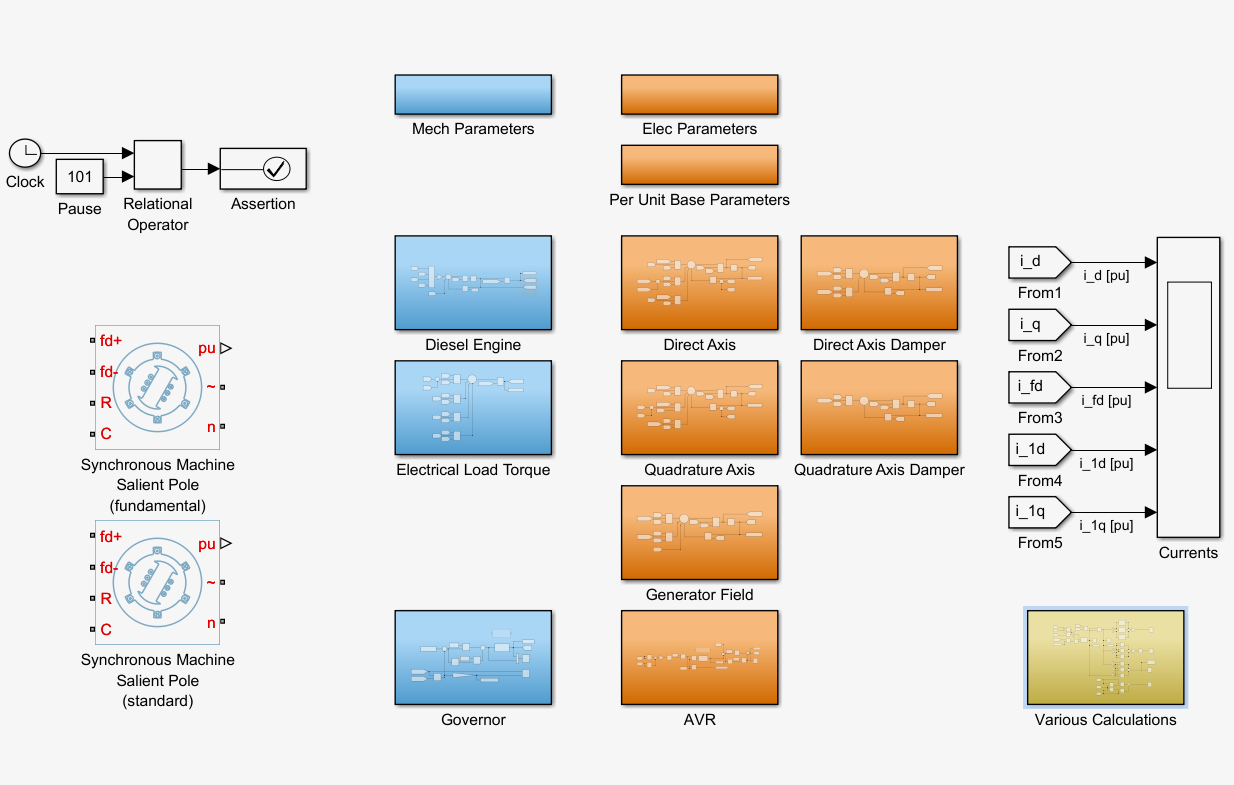
\includegraphics[width=0.75\textwidth]{rapport/billeder/simulink_puOpenLoopDamper}
\caption{Top level of the simulink file, shows the different elements in the model of the genset.}
\label{fig:simulink_puOpenLoopDamper}
\end{figure}

\begin{figure}[H]
\centering
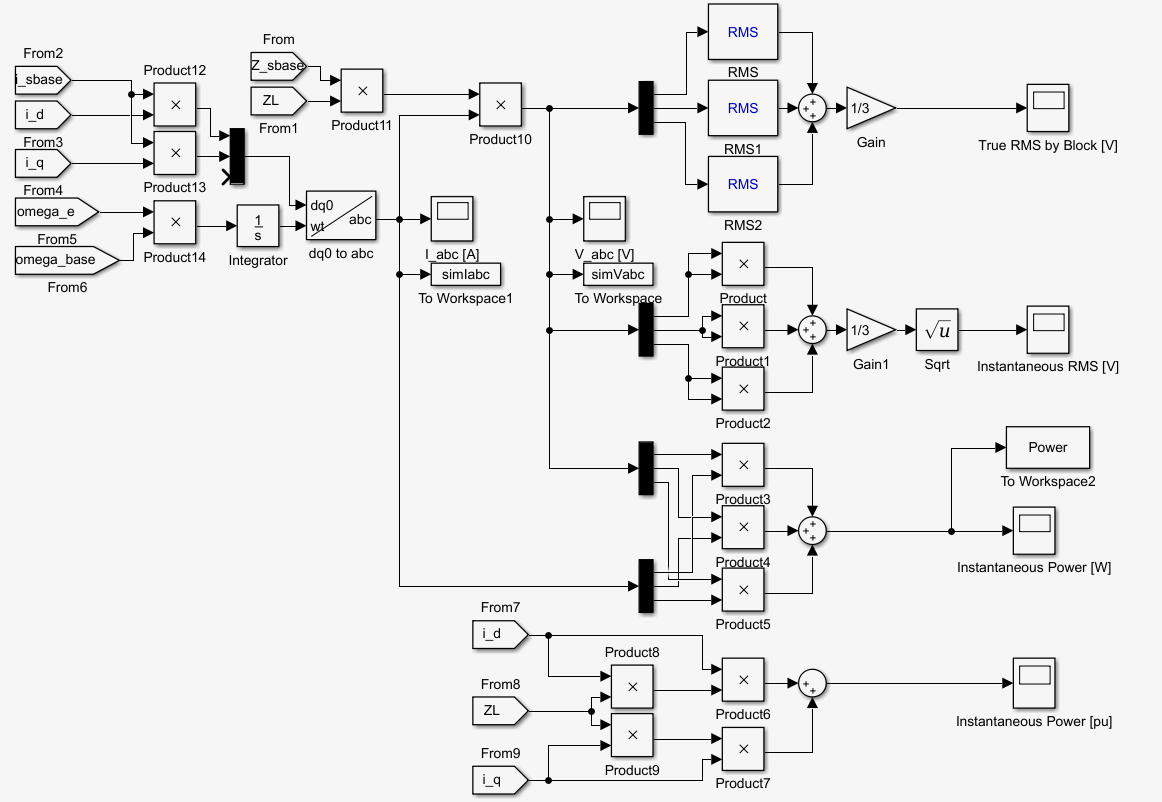
\includegraphics[width=0.75\textwidth]{rapport/billeder/simulink_various_calculations}
\caption{Shows the various calculations of the simulink file, where the V and Power is calculated.}
\label{fig:simulink_various_calculations}
\end{figure}

\begin{figure}[H]
\centering
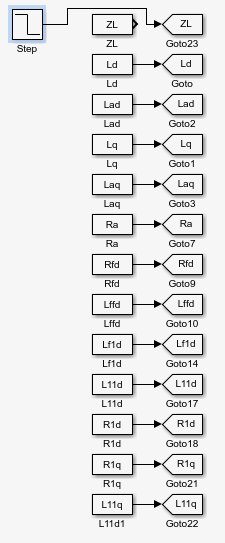
\includegraphics[width=0.3\textwidth]{rapport/billeder/simulink_elec_parameters}
\caption{Shows the Elec. parameters for the genset model. }
\label{fig:simulink_puOpenLoopDamper}
\end{figure}

\begin{equation}
VA_{base} = 60000 \unit{VA}
\end{equation}
\begin{equation}
v_{sbase} = \frac {400 \cdot \sqrt{2}}{\sqrt{3}} \unit{V}
\end{equation}
\begin{equation}
i_{sbase} = \frac {VA_{base}}  {\frac {3}{2} \cdot v_{sbase}} \unit{A}
\end{equation}
\begin{equation}
z_{sbase} = \frac {v_{sbase}}{i_{sbase}} \unit{\Omega}
\end{equation}
\begin{equation}
x_{load} = \frac {400^2}{z_{sbase}\cdot Output_{power}} \unit{\Omega}
\end{equation}

Where:

$VA_{base}$ is Volt-Ampere rating of the machine. $\unit{VA}$

$v_{sbase}$ is Peak phase-to-neutral rated voltage.$\unit{V}$

$i_{sbase}$ is Peak line current.$\unit{A}$

$z_{sbase}$ is Stator base impedance.$\unit{\Omega}$

$x_{load}$ is the load of the grid.$\unit{\Omega}$

$Output_{power}$ is the wanted power output of the genset. $\unit{W}$

By changing $Output_{power}$ it is possible to get different sizes of loads and thereby making a step response. 

\subsection*{Measurement data:}
\begin{figure}[H]
\centering
% This file was created by matlab2tikz.
%
%The latest updates can be retrieved from
%  http://www.mathworks.com/matlabcentral/fileexchange/22022-matlab2tikz-matlab2tikz
%where you can also make suggestions and rate matlab2tikz.
%
\definecolor{mycolor1}{rgb}{0.00000,0.44700,0.74100}%
%
%\begin{tikzpicture}
%
%\begin{axis}[%
%width=4.521in,
%height=3.566in,
%at={(0.758in,0.481in)},
%scale only axis,
%xmin=4.00465520213562,
%xmax=7.12927506355501,
%xlabel={Time (seconds)},
%xmajorgrids,
%ymin=4000,
%ymax=20642.5922346917,
%ylabel={Power (P)},
%ymajorgrids,
%axis background/.style={fill=white},
%title style={font=\bfseries},
%title={Time Series Plot:}
%]
%\addplot [color=mycolor1,solid,forget plot]
%  table[row sep=crcr]{%
%4.004333307996	9918.69016707422\\
%4.00476395020883	9918.69781862561\\
%4.00512539593698	9918.73245921155\\
%4.00550733162754	9918.74225484391\\
%4.00597833824973	9918.73829958975\\
%4.00651402665095	9918.71016064416\\
%4.00689855328635	9918.73176981514\\
%4.00728307992175	9918.74165854259\\
%4.00774997814627	9918.73806813974\\
%4.00827859687631	9918.71266634728\\
%4.00875967965392	9918.68562229758\\
%4.00914933206376	9918.71837567091\\
%4.00951135582634	9918.73929083168\\
%4.00993342547186	9918.74171438305\\
%4.01044501804749	9918.72894046358\\
%4.01096567703278	9918.69016694725\\
%4.01139631924566	9918.69781849896\\
%4.0117577649738	9918.73245908523\\
%4.0121397006643	9918.74225471789\\
%4.01261070728644	9918.73829946408\\
%4.01314639568768	9918.71016051893\\
%4.0135309223231	9918.73176969018\\
%4.01391544895853	9918.7416584179\\
%4.01438234718306	9918.73806801541\\
%4.01491096591305	9918.71266622335\\
%4.01539204869064	9918.68562217401\\
%4.01578170110049	9918.71837554763\\
%4.01614372486311	9918.73929070867\\
%4.01656579450864	9918.74171426036\\
%4.01707738708427	9918.72894034127\\
%4.01759804606953	9918.69016682534\\
%4.01802868828238	9918.69781837738\\
%4.01839013401052	9918.7324589639\\
%4.01877206970105	9918.74225459685\\
%4.01924307632321	9918.7382993434\\
%4.01977876472444	9918.71016039865\\
%4.02016329135984	9918.73176957016\\
%4.02054781799524	9918.74165829818\\
%4.02101471621977	9918.73806789605\\
%4.02154333494979	9918.71266610437\\
%4.02202441772739	9918.68562205537\\
%4.02241407013724	9918.7183754293\\
%4.02277609389983	9918.73929059061\\
%4.02319816354535	9918.74171414261\\
%4.02370975612096	9918.72894022391\\
%4.02423041510622	9918.69016670838\\
%4.02466105731908	9918.69781826071\\
%4.02502250304723	9918.73245884749\\
%4.02540443873775	9918.74225448071\\
%4.0258754453599	9918.73829922759\\
%4.02641113376112	9918.7101602832\\
%4.02679566039655	9918.73176945504\\
%4.02718018703197	9918.74165818332\\
%4.0276470852565	9918.73806778153\\
%4.02817570398649	9918.71266599025\\
%4.02865678676408	9918.68562194162\\
%4.02904643917394	9918.7183753158\\
%4.02940846293655	9918.73929047737\\
%4.02983053258209	9918.74171402967\\
%4.03034212515771	9918.72894011132\\
%4.03086278414297	9918.69016659616\\
%4.03129342635584	9918.69781814882\\
%4.03165487208399	9918.73245873587\\
%4.03203680777452	9918.74225436938\\
%4.03250781439665	9918.7382991166\\
%4.03304350279788	9918.71016017264\\
%4.03342802943331	9918.73176934471\\
%4.03381255606874	9918.74165807329\\
%4.03427945429326	9918.73806767182\\
%4.03480807302325	9918.71266588091\\
%4.03528915580082	9918.68562183264\\
%4.03567880821068	9918.71837520709\\
%4.0360408319733	9918.73929036891\\
%4.03646290161884	9918.7417139215\\
%4.03697449419446	9918.72894000353\\
%4.03749515317973	9918.69016648876\\
%4.03792579539259	9918.69781804171\\
%4.03828724112074	9918.73245862902\\
%4.03866917681126	9918.74225426279\\
%4.0391401834334	9918.73829901033\\
%4.03967587183464	9918.71016006671\\
%4.04006039847007	9918.7317692391\\
%4.0404449251055	9918.74165796793\\
%4.04091182333002	9918.7380675668\\
%4.04144044206001	9918.71266577626\\
%4.04192152483758	9918.68562172834\\
%4.04231117724744	9918.71837510306\\
%4.04267320101005	9918.73929026513\\
%4.04309527065559	9918.74171381803\\
%4.04360686323121	9918.72893990039\\
%4.04412752221645	9918.690166386\\
%4.04455816442931	9918.69781793926\\
%4.04491961015746	9918.7324585268\\
%4.045301545848	9918.74225416082\\
%4.04577255247016	9918.73829890872\\
%4.04630824087139	9918.71015996546\\
%4.0466927675068	9918.7317691381\\
%4.04707729414221	9918.74165786719\\
%4.04754419236673	9918.73806746638\\
%4.04807281109676	9918.71266567624\\
%4.04855389387436	9918.68562162861\\
%4.0489435462842	9918.71837500362\\
%4.04930557004679	9918.73929016594\\
%4.04972763969231	9918.74171371913\\
%4.05023923226794	9918.72893980186\\
%4.05075989125324	9918.69016628776\\
%4.05119053346611	9918.69781784132\\
%4.05155197919424	9918.73245842914\\
%4.05193391488474	9918.74225406343\\
%4.05240492150687	9918.73829881164\\
%4.05294060990812	9918.71015986874\\
%4.05332513654356	9918.73176904165\\
%4.05370966317899	9918.74165777101\\
%4.05417656140352	9918.73806737052\\
%4.0547051801335	9918.71266558073\\
%4.05518626291107	9918.68562153343\\
%4.05557591532092	9918.71837490869\\
%4.05593793908353	9918.73929007124\\
%4.05636000872908	9918.74171362471\\
%4.0568716013047	9918.72893970779\\
%4.05739226028994	9918.69016619408\\
%4.05782290250279	9918.69781774791\\
%4.05818434823094	9918.73245833595\\
%4.05856628392149	9918.74225397049\\
%4.05903729054364	9918.73829871901\\
%4.05957297894486	9918.71015977648\\
%4.05995750558027	9918.73176894964\\
%4.06034203221569	9918.74165767925\\
%4.06080893044023	9918.73806727906\\
%4.06133754917023	9918.71266548958\\
%4.06181863194782	9918.68562144263\\
%4.06220828435767	9918.71837481816\\
%4.06257030812027	9918.73928998096\\
%4.0629923777658	9918.7417135347\\
%4.06350397034143	9918.72893961811\\
%4.0640246293267	9918.69016610474\\
%4.06445527153956	9918.69781765886\\
%4.06481671726771	9918.73245824715\\
%4.06519865295822	9918.74225388194\\
%4.06566965958036	9918.73829863076\\
%4.06620534798161	9918.71015968862\\
%4.06658987461702	9918.73176886199\\
%4.06697440125244	9918.74165759187\\
%4.06744129947696	9918.73806719197\\
%4.06796991820697	9918.71266540284\\
%4.06845100098456	9918.6856213562\\
%4.06884065339441	9918.71837473198\\
%4.06920267715701	9918.73928989501\\
%4.06962474680255	9918.74171344904\\
%4.07013633937817	9918.72893953277\\
%4.07065699836342	9918.69016601972\\
%4.07108764057627	9918.69781757413\\
%4.07144908630442	9918.73245816263\\
%4.07183102199496	9918.74225379769\\
%4.07230202861711	9918.73829854681\\
%4.07283771701831	9918.71015960497\\
%4.07322224365374	9918.73176877863\\
%4.07360677028917	9918.74165750873\\
%4.07407366851368	9918.73806710914\\
%4.07460228724366	9918.71266532037\\
%4.07508337002124	9918.68562127401\\
%4.07547302243111	9918.71837465004\\
%4.07583504619373	9918.73928981329\\
%4.07625711583927	9918.74171336757\\
%4.07676870841487	9918.72893945164\\
%4.07728936740012	9918.69016593893\\
%4.077720009613	9918.69781749359\\
%4.07808145534116	9918.73245808234\\
%4.07846339103169	9918.74225371762\\
%4.07893439765382	9918.73829846703\\
%4.07947008605502	9918.71015952557\\
%4.07985461269046	9918.73176869942\\
%4.0802391393259	9918.74165742977\\
%4.08070603755042	9918.73806703048\\
%4.0812346562804	9918.71266524204\\
%4.08171573905797	9918.685621196\\
%4.08210539146783	9918.71837457224\\
%4.08246741523045	9918.73928973573\\
%4.082889484876	9918.74171329028\\
%4.0834010774516	9918.72893937467\\
%4.08392173643684	9918.69016586227\\
%4.08435237864969	9918.6978174172\\
%4.08471382437786	9918.73245800616\\
%4.08509576006841	9918.74225364166\\
%4.08556676669055	9918.73829839137\\
%4.08610245509174	9918.71015945023\\
%4.08648698172718	9918.73176862434\\
%4.08687150836261	9918.74165735492\\
%4.08733840658713	9918.73806695588\\
%4.08786702531711	9918.71266516778\\
%4.08834810809469	9918.68562112202\\
%4.08873776050456	9918.71837449852\\
%4.08909978426719	9918.73928966222\\
%4.08952185391272	9918.74171321703\\
%4.09003344648832	9918.72893930173\\
%4.09055410547355	9918.69016578965\\
%4.09098474768641	9918.69781734485\\
%4.09134619341458	9918.73245793401\\
%4.09172812910513	9918.74225356977\\
%4.09219913572727	9918.73829831976\\
%4.09273482412847	9918.71015937892\\
%4.0931193507639	9918.73176855326\\
%4.09350387739933	9918.74165728408\\
%4.09397077562384	9918.73806688533\\
%4.09449939435383	9918.71266509753\\
%4.09498047713141	9918.68562105205\\
%4.09537012954128	9918.71837442878\\
%4.0957321533039	9918.7392895927\\
%4.09615422294943	9918.74171314775\\
%4.09666581552503	9918.72893923273\\
%4.09718647451029	9918.69016572099\\
%4.09761711672317	9918.69781727641\\
%4.09797856245133	9918.7324578658\\
%4.09836049814185	9918.74225350177\\
%4.09883150476398	9918.73829825205\\
%4.09936719316519	9918.71015931155\\
%4.09975171980062	9918.73176848609\\
%4.10013624643606	9918.74165721713\\
%4.10060314466058	9918.73806681864\\
%4.10113176339055	9918.71266503115\\
%4.10161284616811	9918.68562098598\\
%4.10200249857798	9918.71837436293\\
%4.10236452234061	9918.73928952704\\
%4.10278659198616	9918.74171308233\\
%4.10329818456177	9918.72893916762\\
%4.10381884354701	9918.69016565615\\
%4.10424948575987	9918.69781721186\\
%4.10461093148803	9918.73245780145\\
%4.10499286717857	9918.74225343762\\
%4.10546387380072	9918.73829818819\\
%4.10599956220192	9918.71015924796\\
%4.10638408883734	9918.73176842275\\
%4.10676861547276	9918.74165715398\\
%4.10723551369728	9918.73806675578\\
%4.10776413242729	9918.71266496861\\
%4.10824521520488	9918.68562092368\\
%4.10863486761473	9918.71837430084\\
%4.10899689137732	9918.73928946517\\
%4.10941896102285	9918.74171302072\\
%4.10993055359847	9918.72893910627\\
%4.11045121258374	9918.69016559512\\
%4.11088185479661	9918.69781715104\\
%4.11124330052477	9918.73245774084\\
%4.11162523621528	9918.74225337725\\
%4.1120962428374	9918.73829812804\\
%4.11263193123861	9918.71015918814\\
%4.11301645787406	9918.73176836314\\
%4.1134009845095	9918.74165709459\\
%4.11386788273402	9918.73806669666\\
%4.11439650146398	9918.71266490978\\
%4.11487758424154	9918.68562086513\\
%4.1152672366514	9918.71837424249\\
%4.11562926041403	9918.73928940702\\
%4.11605133005959	9918.74171296278\\
%4.1165629226352	9918.72893904864\\
%4.1170835816204	9918.69016553777\\
%4.11751422383323	9918.69781709395\\
%4.1178756695614	9918.73245768393\\
%4.11825760525197	9918.74225332052\\
%4.11872861187415	9918.73829807157\\
%4.11926430027534	9918.71015913195\\
%4.11964882691075	9918.73176830717\\
%4.12003335354617	9918.74165703885\\
%4.12050025177068	9918.73806664116\\
%4.12102887050067	9918.71266485453\\
%4.12150995327826	9918.68562081013\\
%4.12189960568813	9918.71837418773\\
%4.12226162945075	9918.73928935246\\
%4.12268369909627	9918.74171290846\\
%4.12319529167187	9918.72893899459\\
%4.12371595065715	9918.690165484\\
%4.12414659287004	9918.69781704037\\
%4.12450803859819	9918.73245763056\\
%4.1248899742887	9918.74225326737\\
%4.12536098091083	9918.73829801867\\
%4.12589666931207	9918.71015907933\\
%4.12628119594751	9918.73176825477\\
%4.12666572258295	9918.74165698664\\
%4.12713262080748	9918.7380665892\\
%4.12766123953747	9918.71266480288\\
%4.12814232231505	9918.68562075872\\
%4.12853197472491	9918.71837413652\\
%4.12889399848752	9918.73928930145\\
%4.12931606813305	9918.74171285765\\
%4.12982766070867	9918.72893894406\\
%4.13034831969393	9918.69016543369\\
%4.13077896190679	9918.69781699034\\
%4.13114040763495	9918.73245758072\\
%4.13152234332548	9918.74225321773\\
%4.13199334994763	9918.73829796929\\
%4.13252903834885	9918.71015903022\\
%4.13291356498427	9918.73176820584\\
%4.13329809161969	9918.74165693792\\
%4.13376498984421	9918.73806654072\\
%4.1342936085742	9918.71266475463\\
%4.13477469135178	9918.68562071074\\
%4.13516434376165	9918.71837408874\\
%4.13552636752427	9918.73928925386\\
%4.1359484371698	9918.74171281031\\
%4.1364600297454	9918.72893889696\\
%4.13698068873063	9918.69016538688\\
%4.13741133094349	9918.69781694375\\
%4.13777277667166	9918.73245753429\\
%4.13815471236221	9918.7422531715\\
%4.13862571898435	9918.73829792328\\
%4.13916140738555	9918.71015898449\\
%4.13954593402099	9918.7317681603\\
%4.13993046065643	9918.74165689257\\
%4.14039735888095	9918.7380664956\\
%4.14092597761092	9918.71266470979\\
%4.1414070603885	9918.68562066614\\
%4.14179671279837	9918.71837404435\\
%4.142158736561	9918.73928920963\\
%4.14258080620654	9918.74171276627\\
%4.14309239878214	9918.7289388532\\
%4.14361305776737	9918.69016534341\\
%4.14404369998023	9918.69781690045\\
%4.1444051457084	9918.73245749118\\
%4.14478708139894	9918.74225312857\\
%4.14525808802108	9918.73829788058\\
%4.14579377642228	9918.71015894206\\
%4.14617830305772	9918.73176811806\\
%4.14656282969316	9918.74165685051\\
%4.14702972791768	9918.73806645379\\
%4.14755834664766	9918.71266466823\\
%4.14803942942524	9918.68562062482\\
%4.14842908183511	9918.71837400321\\
%4.14879110559773	9918.73928916867\\
%4.14921317524327	9918.74171272552\\
%4.14972476781888	9918.72893881268\\
%4.15024542680413	9918.69016530314\\
%4.15067606901699	9918.6978168604\\
%4.15103751474516	9918.73245745132\\
%4.15141945043568	9918.74225308888\\
%4.15189045705782	9918.73829784113\\
%4.15242614545902	9918.71015890288\\
%4.15281067209446	9918.73176807904\\
%4.15319519872991	9918.74165681169\\
%4.15366209695442	9918.73806641518\\
%4.15419071568437	9918.71266462991\\
%4.15467179846192	9918.68562058673\\
%4.15506145087178	9918.71837396526\\
%4.15542347463443	9918.73928913089\\
%4.15584554427999	9918.74171268793\\
%4.1563571368556	9918.72893877535\\
%4.15687779584078	9918.69016526604\\
%4.1573084380536	9918.69781682354\\
%4.15766988378177	9918.73245741458\\
%4.15805181947236	9918.74225305231\\
%4.15852282609454	9918.73829780476\\
%4.15905851449573	9918.71015886675\\
%4.15944304113115	9918.73176804312\\
%4.15982756776656	9918.74165677595\\
%4.16029446599108	9918.73806637965\\
%4.16082308472107	9918.7126645946\\
%4.16130416749866	9918.68562055164\\
%4.16169381990852	9918.71837393038\\
%4.16205584367113	9918.73928909618\\
%4.16247791331666	9918.74171265342\\
%4.16298950589227	9918.72893874106\\
%4.16351016487754	9918.69016523199\\
%4.16394080709041	9918.69781678963\\
%4.16430225281857	9918.73245738088\\
%4.16468418850908	9918.74225301881\\
%4.16515519513121	9918.73829777149\\
%4.16569088353244	9918.71015883369\\
%4.16607541016788	9918.73176801024\\
%4.16645993680332	9918.74165674325\\
%4.16692683502784	9918.73806634717\\
%4.16745545375779	9918.71266456237\\
%4.16793653653535	9918.68562051963\\
%4.16832618894521	9918.71837389854\\
%4.16868821270785	9918.73928906448\\
%4.16911028235341	9918.7417126219\\
%4.16962187492902	9918.72893870978\\
%4.17014253391425	9918.69016520093\\
%4.17057317612708	9918.69781675879\\
%4.17093462185524	9918.73245735018\\
%4.17131655754579	9918.74225298827\\
%4.17178756416797	9918.73829774115\\
%4.17232325256917	9918.7101588036\\
%4.17270777920459	9918.73176798032\\
%4.17309230584	9918.74165671349\\
%4.17355920406451	9918.7380663176\\
%4.1740878227945	9918.71266453304\\
%4.17456890557209	9918.68562049048\\
%4.17495855798196	9918.71837386957\\
%4.17532058174457	9918.7392890357\\
%4.1757426513901	9918.74171259331\\
%4.17625424396571	9918.7289386814\\
%4.17677490295096	9918.69016517279\\
%4.17720554516382	9918.69781673082\\
%4.17756699089198	9918.73245732237\\
%4.17794892658251	9918.74225296063\\
%4.17841993320465	9918.73829771371\\
%4.17895562160588	9918.7101587764\\
%4.1793401482413	9918.73176795328\\
%4.17972467487673	9918.74165668661\\
%4.18019157310125	9918.73806629092\\
%4.18072019183124	9918.71266450656\\
%4.18120127460883	9918.68562046421\\
%4.18159092701869	9918.71837384348\\
%4.1819529507813	9918.73928900975\\
%4.18237502042683	9918.74171256753\\
%4.18288661300245	9918.72893865586\\
%4.18340727198771	9918.69016514743\\
%4.18383791420056	9918.69781670565\\
%4.18419935992871	9918.73245729737\\
%4.18458129561925	9918.74225293579\\
%4.1850523022414	9918.73829768909\\
%4.18558799064263	9918.71015875198\\
%4.18597251727804	9918.73176792902\\
%4.18635704391346	9918.74165666251\\
%4.18682394213798	9918.73806626701\\
%4.18735256086799	9918.71266448286\\
%4.18783364364558	9918.68562044071\\
%4.18822329605544	9918.71837382015\\
%4.18858531981804	9918.73928898656\\
%4.18900738946357	9918.74171254452\\
%4.18951898203919	9918.72893863304\\
%4.19003964102445	9918.69016512485\\
%4.19047028323732	9918.69781668323\\
%4.19083172896547	9918.73245727509\\
%4.19121366465599	9918.74225291367\\
%4.19168467127813	9918.73829766714\\
%4.19222035967935	9918.71015873025\\
%4.19260488631478	9918.73176790744\\
%4.19298941295021	9918.74165664109\\
%4.19345631117474	9918.73806624578\\
%4.19398492990473	9918.71266446186\\
%4.19446601268231	9918.6856204199\\
%4.19485566509216	9918.71837379946\\
%4.19521768885477	9918.73928896603\\
%4.19563975850031	9918.74171252415\\
%4.19615135107594	9918.72893861287\\
%4.19667201006121	9918.69016510486\\
%4.19710265227406	9918.69781666344\\
%4.19746409800221	9918.73245725544\\
%4.19784603369273	9918.74225289416\\
%4.19831704031489	9918.73829764781\\
%4.19885272871614	9918.71015871115\\
%4.19923725535155	9918.73176788849\\
%4.19962178198697	9918.74165662229\\
%4.2000886802115	9918.73806622715\\
%4.20061729894152	9918.71266444341\\
%4.20109838171913	9918.68562040163\\
%4.20148803412897	9918.71837378139\\
%4.20185005789156	9918.7392889481\\
%4.20227212753708	9918.74171250639\\
%4.2027837201127	9918.72893859529\\
%4.20330437909799	9918.69016508749\\
%4.20373502131087	9918.6978166462\\
%4.20409646703901	9918.73245723836\\
%4.20447840272951	9918.74225287723\\
%4.20494940935165	9918.73829763108\\
%4.2054850977529	9918.7101586946\\
%4.20586962438832	9918.73176787208\\
%4.20625415102375	9918.74165660601\\
%4.20672104924828	9918.73806621107\\
%4.20724966797828	9918.71266442752\\
%4.20773075075585	9918.68562038594\\
%4.2081204031657	9918.71837376583\\
%4.20848242692831	9918.73928893266\\
%4.20890449657385	9918.7417124911\\
%4.20941608914948	9918.72893858017\\
%4.20993674813474	9918.69016507259\\
%4.2103673903476	9918.69781663149\\
%4.21072883607575	9918.73245722375\\
%4.21111077176627	9918.74225286276\\
%4.21158177838842	9918.73829761676\\
%4.21211746678965	9918.71015868048\\
%4.21250199342507	9918.73176785811\\
%4.2128865200605	9918.7416565922\\
%4.21335341828502	9918.7380661974\\
%4.21388203701501	9918.71266441406\\
%4.21436311979259	9918.68562037265\\
%4.21475277220245	9918.71837375267\\
%4.21511479596506	9918.73928891962\\
%4.2155368656106	9918.74171247823\\
%4.2160484581862	9918.72893856751\\
%4.21656911717144	9918.69016506009\\
%4.21699975938431	9918.69781661915\\
%4.21736120511247	9918.73245721154\\
%4.21774314080301	9918.74225285068\\
%4.21821414742515	9918.73829760485\\
%4.21874983582635	9918.71015866878\\
%4.21913436246178	9918.73176784652\\
%4.21951888909721	9918.74165658074\\
%4.21998578732173	9918.73806618612\\
%4.22051440605172	9918.71266440295\\
%4.2209954888293	9918.68562036172\\
%4.22138514123915	9918.71837374186\\
%4.22174716500177	9918.73928890895\\
%4.22216923464731	9918.74171246769\\
%4.22268082722293	9918.72893855716\\
%4.22320148620818	9918.69016504993\\
%4.22363212842102	9918.69781660911\\
%4.22399357414917	9918.73245720163\\
%4.22437550983972	9918.74225284089\\
%4.22484651646188	9918.73829759522\\
%4.22538220486311	9918.71015865932\\
%4.22576673149852	9918.73176783721\\
%4.22615125813394	9918.74165657156\\
%4.22661815635847	9918.73806617711\\
%4.22714677508847	9918.71266439412\\
%4.22762785786605	9918.68562035303\\
%4.22801751027589	9918.71837373332\\
%4.2283795340385	9918.73928890054\\
%4.22880160368404	9918.74171245942\\
%4.22931319625966	9918.72893854905\\
%4.22983385524491	9918.69016504199\\
%4.23026449745777	9918.69781660133\\
%4.23062594318592	9918.73245719397\\
%4.23100787887646	9918.74225283337\\
%4.23147888549861	9918.73829758786\\
%4.23201457389983	9918.71015865213\\
%4.23239910053526	9918.73176783015\\
%4.23278362717068	9918.74165656463\\
%4.2332505253952	9918.73806617032\\
%4.23377914412518	9918.71266438753\\
%4.23426022690275	9918.6856203466\\
%4.23464987931261	9918.71837372699\\
%4.23501190307523	9918.73928889432\\
%4.23543397272077	9918.74171245333\\
%4.23594556529639	9918.72893854313\\
%4.23646622428164	9918.69016503625\\
%4.2368968664945	9918.69781659573\\
%4.23725831222265	9918.73245718846\\
%4.23764024791318	9918.74225282799\\
%4.23811125453534	9918.73829758264\\
%4.23864694293657	9918.71015864706\\
%4.23903146957199	9918.73176782521\\
%4.23941599620741	9918.74165655982\\
%4.23988289443194	9918.73806616567\\
%4.24041151316194	9918.71266438301\\
%4.24089259593951	9918.68562034223\\
%4.24128224834937	9918.71837372278\\
%4.24164427211198	9918.73928889023\\
%4.24206634175753	9918.74171244937\\
%4.24257793433314	9918.72893853934\\
%4.24309859331839	9918.6901650326\\
%4.24352923553124	9918.6978165922\\
%4.2438906812594	9918.73245718507\\
%4.24427261694993	9918.7422528247\\
%4.24474362357209	9918.73829757949\\
%4.24527931197331	9918.71015864406\\
%4.24566383860874	9918.73176782235\\
%4.24604836524417	9918.74165655707\\
%4.24651526346869	9918.73806616305\\
%4.24704388219867	9918.71266438056\\
%4.24752496497626	9918.68562033994\\
%4.24791461738613	9918.71837372059\\
%4.24827664114875	9918.73928888814\\
%4.24869871079428	9918.74171244743\\
%4.24921030336988	9918.72893853753\\
%4.24973096235515	9918.69016503095\\
%4.25016160456802	9918.69781659068\\
%4.25052305029619	9918.73245718367\\
%4.25090498598671	9918.74225282343\\
%4.25137599260884	9918.73829757836\\
%4.25191168101006	9918.71015864313\\
%4.2522962076455	9918.73176782149\\
%4.25268073428093	9918.74165655631\\
%4.25314763250545	9918.73806616243\\
%4.25367625123543	9918.71266438011\\
%4.254157334013	9918.68562033962\\
%4.25454698642286	9918.71837372037\\
%4.25490901018549	9918.73928888803\\
%4.25533107983104	9918.74171244743\\
%4.25584267240665	9918.72893853769\\
%4.2563633313919	9918.69016503126\\
%4.25679397360476	9918.69781659113\\
%4.25715541933292	9918.73245718421\\
%4.25753735502346	9918.74225282408\\
%4.25800836164561	9918.73829757914\\
%4.25854405004679	9918.71015864405\\
%4.25892857668223	9918.73176782253\\
%4.25931310331766	9918.74165655747\\
%4.25978000154217	9918.73806616373\\
%4.26030862027212	9918.71266438157\\
%4.26078970304968	9918.68562034122\\
%4.26117935545956	9918.71837372206\\
%4.2615413792222	9918.73928888982\\
%4.26196344886775	9918.74171244934\\
%4.26247504144333	9918.72893853973\\
%4.26299570042854	9918.6901650335\\
%4.2634263426414	9918.69781659346\\
%4.26378778836958	9918.73245718662\\
%4.26416972406014	9918.74225282658\\
%4.26464073068229	9918.73829758177\\
%4.26517641908347	9918.71015864682\\
%4.26556094571892	9918.73176782541\\
%4.26594547235436	9918.74165656045\\
%4.26641237057887	9918.73806616682\\
%4.26694098930884	9918.7126643848\\
%4.26742207208643	9918.68562034458\\
%4.26781172449631	9918.71837372555\\
%4.26817374825894	9918.7392888934\\
%4.26859581790446	9918.74171245304\\
%4.26910741048004	9918.72893854359\\
%4.26962806946529	9918.69016503747\\
%4.27005871167817	9918.69781659753\\
%4.27042015740635	9918.7324571908\\
%4.27080209309688	9918.74225283087\\
%4.27127309971901	9918.73829758619\\
%4.27180878812021	9918.71015865141\\
%4.27219331475565	9918.73176783007\\
%4.2725778413911	9918.74165656521\\
%4.27304473961562	9918.73806617171\\
%4.27357335834559	9918.71266438983\\
%4.27405444112316	9918.68562034974\\
%4.27444409353303	9918.7183737308\\
%4.27480611729566	9918.73928889875\\
%4.2752281869412	9918.74171245848\\
%4.27573977951682	9918.72893854915\\
%4.27626043850206	9918.69016504317\\
%4.27669108071491	9918.69781660335\\
%4.27705252644307	9918.73245719671\\
%4.27743446213361	9918.74225283687\\
%4.27790546875576	9918.73829759231\\
%4.27844115715698	9918.71015865764\\
%4.27882568379241	9918.73176783643\\
%4.27921021042783	9918.74165657166\\
%4.27967710865235	9918.73806617828\\
%4.28020572738235	9918.71266439653\\
%4.28068681015994	9918.68562035654\\
%4.2810764625698	9918.71837373771\\
%4.2814384863324	9918.73928890574\\
%4.28186055597793	9918.74171246559\\
%4.28237214855355	9918.72893855636\\
%4.28289280753882	9918.69016505048\\
%4.28332344975169	9918.69781661079\\
%4.28368489547984	9918.73245720426\\
%4.28406683117035	9918.74225284451\\
%4.2845378377925	9918.73829760006\\
%4.28507352619373	9918.71015866553\\
%4.28545805282916	9918.73176784441\\
%4.28584257946459	9918.74165657973\\
%4.28630947768913	9918.73806618646\\
%4.28683809641913	9918.71266440484\\
%4.28731917919671	9918.68562036496\\
%4.28770883160655	9918.71837374622\\
%4.28807085536916	9918.73928891435\\
%4.28849292501469	9918.7417124743\\
%4.28900451759033	9918.72893856521\\
%4.28952517657559	9918.69016505943\\
%4.28995581878843	9918.69781661985\\
%4.29031726451657	9918.7324572134\\
%4.2906992002071	9918.74225285373\\
%4.29117020682927	9918.7382976094\\
%4.29170589523051	9918.71015867498\\
%4.29209042186591	9918.73176785395\\
%4.29247494850132	9918.74165658938\\
%4.29294184672584	9918.73806619622\\
%4.29347046545585	9918.71266441469\\
%4.29395154823345	9918.68562037493\\
%4.2943412006433	9918.71837375628\\
%4.29470322440589	9918.73928892449\\
%4.29512529405142	9918.74171248454\\
%4.29563688662704	9918.72893857557\\
%4.29615754561232	9918.69016506992\\
%4.29658818782518	9918.69781663041\\
%4.29694963355333	9918.73245722404\\
%4.29733156924384	9918.74225286448\\
%4.29780257586598	9918.73829762024\\
%4.29833826426722	9918.71015868596\\
%4.29872279090265	9918.731767865\\
%4.29910731753808	9918.7416566005\\
%4.2995742157626	9918.73806620744\\
%4.30010283449259	9918.71266442605\\
%4.30058391727017	9918.6856203864\\
%4.30097356968003	9918.71837376784\\
%4.30133559344264	9918.73928893611\\
%4.30175766308818	9918.74171249625\\
%4.30226925566381	9918.72893858736\\
%4.30278991464909	9918.69016508182\\
%4.30322055686196	9918.69781664243\\
%4.30358200259011	9918.73245723615\\
%4.30396393828062	9918.74225287667\\
%4.30443494490275	9918.73829763253\\
%4.30497063330397	9918.71015869837\\
%4.30535515993941	9918.73176787748\\
%4.30573968657485	9918.74165661306\\
%4.30620658479938	9918.73806622008\\
%4.30673520352938	9918.71266443881\\
%4.30721628630696	9918.68562039924\\
%4.3076059387168	9918.71837378078\\
%4.30796796247941	9918.73928894913\\
%4.30839003212495	9918.74171250936\\
%4.30890162470057	9918.72893860059\\
%4.30942228368584	9918.69016509515\\
%4.3098529258987	9918.69781665585\\
%4.31021437162685	9918.73245724963\\
%4.31059630731737	9918.74225289022\\
%4.31106731393951	9918.73829764617\\
%4.31160300234074	9918.71015871209\\
%4.31198752897618	9918.73176789131\\
%4.31237205561162	9918.74165662697\\
%4.31283895383614	9918.73806623411\\
%4.31336757256612	9918.71266445293\\
%4.31384865534369	9918.68562041349\\
%4.31423830775355	9918.71837379506\\
%4.31460033151617	9918.7392889635\\
%4.31502240116171	9918.7417125238\\
%4.31553399373733	9918.72893861515\\
%4.31605465272256	9918.69016510983\\
%4.31648529493541	9918.69781667061\\
%4.31684674066357	9918.73245726443\\
%4.31722867635412	9918.7422529051\\
%4.31769968297628	9918.73829766115\\
%4.31823537137749	9918.71015872718\\
%4.31861989801292	9918.73176790646\\
%4.31900442464834	9918.7416566422\\
%4.31947132287287	9918.7380662494\\
%4.31999994160288	9918.71266446831\\
%4.32048102438048	9918.68562042895\\
%4.32087067679034	9918.71837381065\\
%4.32123270055294	9918.73928897915\\
%4.32165477019846	9918.74171253954\\
%4.32216636277408	9918.72893863097\\
%4.32268702175935	9918.69016512574\\
%4.32311766397223	9918.69781668658\\
%4.32347910970038	9918.7324572805\\
%4.32386104539089	9918.74225292124\\
%4.32433205201303	9918.73829767736\\
%4.32486774041428	9918.7101587435\\
%4.32525226704971	9918.73176792285\\
%4.32563679368514	9918.74165665865\\
%4.32610369190967	9918.73806626597\\
%4.32663231063966	9918.71266448498\\
%4.32711339341724	9918.68562044571\\
%4.32750304582709	9918.71837382745\\
%4.32786506958971	9918.73928899601\\
%4.32828713923524	9918.74171255647\\
%4.32879873181085	9918.72893864802\\
%4.32931939079609	9918.69016514289\\
%4.32975003300894	9918.6978167038\\
%4.3301114787371	9918.73245729777\\
%4.33049341442765	9918.74225293856\\
%4.33096442104981	9918.73829769478\\
%4.33150010945104	9918.71015876098\\
%4.33188463608646	9918.73176794043\\
%4.33226916272188	9918.7416566763\\
%4.3327360609464	9918.73806628369\\
%4.33326467967639	9918.71266450281\\
%4.33374576245397	9918.6856204636\\
%4.33413541486382	9918.7183738454\\
%4.33449743862643	9918.73928901402\\
%4.33491950827197	9918.74171257454\\
%4.3354311008476	9918.72893866614\\
%4.33595175983287	9918.69016516113\\
%4.33638240204573	9918.69781672211\\
%4.33674384777388	9918.73245731615\\
%4.33712578346439	9918.74225295702\\
%4.33759679008654	9918.73829771333\\
%4.33813247848778	9918.71015877966\\
%4.33851700512319	9918.73176795913\\
%4.3389015317586	9918.74165669505\\
%4.33936842998313	9918.73806630252\\
%4.33989704871315	9918.71266452168\\
%4.34037813149073	9918.68562048256\\
%4.34076778390058	9918.71837386445\\
%4.34112980766318	9918.73928903314\\
%4.34155187730871	9918.74171259374\\
%4.34206346988433	9918.72893868545\\
%4.34258412886959	9918.69016518048\\
%4.34301477108245	9918.69781674153\\
%4.3433762168106	9918.73245733563\\
%4.34375815250112	9918.74225297656\\
%4.34422915912327	9918.73829773294\\
%4.3447648475245	9918.71015879932\\
%4.34514937415992	9918.73176797887\\
%4.34553390079534	9918.74165671486\\
%4.34600079901986	9918.73806632239\\
%4.34652941774985	9918.71266454166\\
%4.34701050052744	9918.68562050263\\
%4.3474001529373	9918.71837388455\\
%4.34776217669991	9918.73928905329\\
%4.34818424634543	9918.74171261395\\
%4.34869583892103	9918.72893870574\\
%4.3492164979063	9918.69016520086\\
%4.34964714011917	9918.69781676198\\
%4.35000858584733	9918.73245735612\\
%4.35039052153785	9918.7422529971\\
%4.35086152815997	9918.73829775355\\
%4.35139721656119	9918.71015882004\\
%4.35178174319663	9918.73176799962\\
%4.35216626983208	9918.74165673567\\
%4.3526331680566	9918.73806634326\\
%4.35316178678656	9918.71266456264\\
%4.35364286956414	9918.68562052368\\
%4.35403252197401	9918.71837390564\\
%4.35439454573664	9918.73928907443\\
%4.35481661538217	9918.74171263515\\
%4.35532820795777	9918.728938727\\
%4.355848866943	9918.69016522224\\
%4.35627950915585	9918.6978167834\\
%4.35664095488402	9918.73245737758\\
%4.35702289057457	9918.74225301861\\
%4.35749389719672	9918.73829777512\\
%4.35802958559792	9918.71015884167\\
%4.35841411223335	9918.73176802131\\
%4.35879863886877	9918.74165675743\\
%4.3592655370933	9918.7380663651\\
%4.3597941558233	9918.71266458451\\
%4.36027523860088	9918.68562054561\\
%4.36066489101074	9918.71837392765\\
%4.36102691477334	9918.73928909649\\
%4.36144898441888	9918.74171265726\\
%4.3619605769945	9918.72893874919\\
%4.36248123597976	9918.69016524446\\
%4.36291187819261	9918.69781680569\\
%4.36327332392076	9918.73245739994\\
%4.36365525961128	9918.74225304103\\
%4.36412626623344	9918.7382977976\\
%4.36466195463467	9918.71015886422\\
%4.36504648127008	9918.73176804393\\
%4.3654310079055	9918.74165678008\\
%4.36589790613003	9918.73806638781\\
%4.36642652486003	9918.71266460732\\
%4.36690760763761	9918.68562056843\\
%4.36729726004746	9918.71837395053\\
%4.36765928381006	9918.73928911943\\
%4.3680813534556	9918.74171268025\\
%4.36859294603123	9918.72893877223\\
%4.36911360501648	9918.69016526757\\
%4.36954424722932	9918.69781682886\\
%4.36990569295747	9918.73245742316\\
%4.37028762864801	9918.74225306429\\
%4.37075863527017	9918.73829782092\\
%4.3712943236714	9918.71015888762\\
%4.37167885030681	9918.73176806737\\
%4.37206337694222	9918.74165680357\\
%4.37253027516674	9918.73806641134\\
%4.37305889389674	9918.71266463089\\
%4.37353997667434	9918.6856205921\\
%4.3739296290842	9918.71837397424\\
%4.37429165284681	9918.73928914317\\
%4.37471372249233	9918.74171270408\\
%4.37522531506793	9918.72893879612\\
%4.37574597405318	9918.6901652915\\
%4.37617661626604	9918.69781685285\\
%4.37653806199421	9918.73245744717\\
%4.37691999768474	9918.74225308836\\
%4.37739100430689	9918.73829784506\\
%4.3779266927081	9918.7101589118\\
%4.37831121934352	9918.73176809159\\
%4.37869574597895	9918.74165682783\\
%4.37916264420347	9918.73806643566\\
%4.37969126293348	9918.71266465526\\
%4.38017234571108	9918.68562061653\\
%4.38056199812094	9918.71837399872\\
%4.38092402188354	9918.73928916771\\
%4.38134609152905	9918.74171272864\\
%4.38185768410466	9918.72893882074\\
%4.38237834308994	9918.6901653162\\
%4.38280898530281	9918.69781687757\\
%4.38317043103096	9918.73245747195\\
%4.38355236672147	9918.74225311317\\
%4.38402337334361	9918.73829786991\\
%4.38455906174483	9918.71015893675\\
%4.38494358838026	9918.73176811656\\
%4.38532811501568	9918.74165685284\\
%4.3857950132402	9918.73806646074\\
%4.38632363197019	9918.7126646804\\
%4.38680471474776	9918.68562064173\\
%4.38719436715762	9918.71837402392\\
%4.38755639092023	9918.73928919294\\
%4.38797846056578	9918.74171275392\\
%4.38849005314141	9918.72893884606\\
%4.38901071212667	9918.69016534157\\
%4.38944135433952	9918.69781690301\\
%4.38980280006767	9918.73245749742\\
%4.39018473575819	9918.74225313867\\
%4.39065574238036	9918.73829789548\\
%4.3911914307816	9918.71015896233\\
%4.391575957417	9918.73176814219\\
%4.39196048405241	9918.74165687852\\
%4.39242738227694	9918.73806648647\\
%4.39295600100697	9918.71266470619\\
%4.39343708378455	9918.68562066753\\
%4.39382673619439	9918.71837404981\\
%4.39418875995698	9918.73928921886\\
%4.39461082960251	9918.74171277987\\
%4.39512242217815	9918.72893887207\\
%4.39564308116343	9918.6901653676\\
%4.3960737233763	9918.69781692908\\
%4.39643516910443	9918.73245752355\\
%4.39681710479494	9918.74225316485\\
%4.39728811141708	9918.73829792168\\
%4.39782379981832	9918.7101589886\\
%4.39820832645374	9918.73176816851\\
%4.39859285308917	9918.74165690485\\
%4.39905975131369	9918.73806651282\\
%4.3995883700437	9918.71266473261\\
%4.40006945282128	9918.68562069401\\
%4.40045910523113	9918.71837407631\\
%4.40082112899374	9918.73928924539\\
%4.40124319863927	9918.74171280644\\
%4.4017547912149	9918.7289388987\\
%4.40227545020015	9918.6901653943\\
%4.40270609241299	9918.69781695582\\
%4.40306753814113	9918.73245755029\\
%4.40344947383166	9918.74225319161\\
%4.40392048045382	9918.73829794849\\
%4.40445616885505	9918.71015901544\\
%4.40484069549046	9918.73176819538\\
%4.40522522212587	9918.74165693178\\
%4.40569212035039	9918.73806653981\\
%4.40622073908041	9918.71266475961\\
%4.40670182185799	9918.68562072106\\
%4.40709147426783	9918.71837410338\\
%4.40745349803042	9918.73928927249\\
%4.40787556767596	9918.74171283359\\
%4.40838716025158	9918.72893892588\\
%4.40890781923683	9918.69016542153\\
%4.40933846144968	9918.69781698307\\
%4.40969990717783	9918.73245757758\\
%4.41008184286837	9918.74225321894\\
%4.41055284949053	9918.73829797585\\
%4.41108853789175	9918.71015904286\\
%4.41147306452716	9918.73176822283\\
%4.41185759116257	9918.74165695925\\
%4.41232448938709	9918.73806656729\\
%4.4128531081171	9918.71266478716\\
%4.41333419089471	9918.68562074863\\
%4.41372384330456	9918.71837413099\\
%4.41408586706715	9918.73928930014\\
%4.41450793671267	9918.74171286126\\
%4.41501952928828	9918.72893895361\\
%4.41554018827356	9918.69016544928\\
%4.41597083048643	9918.69781701085\\
%4.41633227621457	9918.73245760539\\
%4.41671421190508	9918.74225324677\\
%4.41718521852722	9918.73829800372\\
%4.41772090692847	9918.71015907073\\
%4.4181054335639	9918.73176825074\\
%4.41848996019933	9918.7416569872\\
%4.41895685842387	9918.73806659528\\
%4.41948547715389	9918.71266481516\\
%4.41996655993149	9918.6856207767\\
%4.42035621234134	9918.7183741591\\
%4.42071823610393	9918.73928932826\\
%4.42114030574946	9918.74171288942\\
%4.42165189832508	9918.72893898177\\
%4.42217255731036	9918.69016547749\\
%4.42260319952323	9918.6978170391\\
%4.42296464525137	9918.73245763367\\
%4.42334658094189	9918.74225327509\\
%4.42381758756403	9918.73829803206\\
%4.42435327596526	9918.71015909915\\
%4.42473780260069	9918.73176827917\\
%4.42512232923612	9918.74165701565\\
%4.42558922746064	9918.73806662376\\
%4.42611784619063	9918.71266484368\\
%4.4265989289682	9918.68562080524\\
%4.42698858137805	9918.71837418766\\
%4.42735060514067	9918.73928935684\\
%4.42777267478622	9918.74171291802\\
%4.42828426736183	9918.72893901039\\
%4.42880492634707	9918.69016550614\\
%4.42923556855994	9918.69781706779\\
%4.42959701428811	9918.73245766237\\
%4.42997894997865	9918.74225330381\\
%4.43044995660079	9918.73829806083\\
%4.43098564500198	9918.71015912796\\
%4.43137017163741	9918.73176830797\\
%4.43175469827284	9918.74165704447\\
%4.43222159649736	9918.73806665262\\
%4.43275021522734	9918.71266487259\\
%4.43323129800491	9918.6856208342\\
%4.43362095041476	9918.71837421659\\
%4.43398297417738	9918.73928938579\\
%4.43440504382293	9918.74171294698\\
%4.43491663639855	9918.7289390394\\
%4.43543729538381	9918.69016553518\\
%4.43586793759667	9918.69781709686\\
%4.43622938332483	9918.73245769146\\
%4.43661131901535	9918.74225333293\\
%4.4370823256375	9918.73829808996\\
%4.43761801403873	9918.71015915709\\
%4.43800254067416	9918.73176833716\\
%4.43838706730959	9918.74165707368\\
%4.43885396553411	9918.73806668185\\
%4.43938258426409	9918.71266490183\\
%4.43986366704168	9918.68562086345\\
%4.44025331945154	9918.71837424589\\
%4.44061534321416	9918.73928941512\\
%4.44103741285969	9918.74171297634\\
%4.4415490054353	9918.72893906879\\
%4.44206966442055	9918.6901655646\\
%4.44250030663342	9918.69781712628\\
%4.44286175236158	9918.7324577209\\
%4.44324368805211	9918.74225336239\\
%4.44371469467424	9918.73829811944\\
%4.44425038307542	9918.71015918663\\
%4.44463490971087	9918.73176836668\\
%4.44501943634631	9918.74165710321\\
%4.44548633457083	9918.73806671139\\
%4.4460149533008	9918.71266493141\\
%4.44649603607839	9918.68562089306\\
%4.44688568848827	9918.71837427551\\
%4.4472477122509	9918.73928944475\\
%4.44766978189642	9918.74171300601\\
%4.44818137447202	9918.72893909849\\
%4.44870203345726	9918.69016559434\\
%4.44913267567012	9918.69781715603\\
%4.44949412139829	9918.73245775065\\
%4.44987605708883	9918.74225339216\\
%4.45034706371098	9918.73829814921\\
%4.45088275211218	9918.71015921641\\
%4.45126727874761	9918.73176839652\\
%4.45165180538305	9918.74165713307\\
%4.45211870360757	9918.73806674128\\
%4.45264732233753	9918.71266496134\\
%4.45312840511509	9918.68562092299\\
%4.45351805752495	9918.71837430546\\
%4.45388008128759	9918.7392894747\\
%4.45430215093314	9918.74171303596\\
%4.45481374350874	9918.72893912843\\
%4.45533440249396	9918.6901656243\\
%4.45576504470683	9918.69781718604\\
%4.456126490435	9918.73245778066\\
%4.45650842612555	9918.74225342217\\
%4.4569794327477	9918.73829817927\\
%4.4575151211489	9918.71015924648\\
%4.45789964778433	9918.7317684266\\
%4.45828417441976	9918.74165716317\\
%4.45875107264427	9918.73806677139\\
%4.45927969137425	9918.71266499148\\
%4.45976077415182	9918.68562095314\\
%4.46015042656169	9918.71837433562\\
%4.46051245032431	9918.73928950488\\
%4.46093451996985	9918.74171306615\\
%4.46144611254544	9918.72893915869\\
%4.46196677153067	9918.69016565456\\
%4.46239741374352	9918.69781721629\\
%4.46275885947169	9918.73245781093\\
%4.46314079516224	9918.74225345245\\
%4.46361180178439	9918.73829820956\\
%4.4641474901856	9918.71015927679\\
%4.46453201682103	9918.7317684569\\
%4.46491654345646	9918.74165719348\\
%4.46538344168098	9918.73806680171\\
%4.46591206041099	9918.71266502179\\
%4.46639314318858	9918.68562098347\\
%4.46678279559843	9918.718374366\\
%4.46714481936103	9918.73928953527\\
%4.46756688900656	9918.74171309656\\
%4.46807848158218	9918.72893918908\\
%4.46859914056744	9918.69016568498\\
%4.46902978278031	9918.69781724671\\
%4.46939122850846	9918.73245784137\\
%4.46977316419898	9918.74225348291\\
%4.47024417082112	9918.73829824002\\
%4.47077985922237	9918.71015930726\\
%4.4711643858578	9918.7317684874\\
%4.47154891249323	9918.74165722399\\
%4.47201581071776	9918.73806683226\\
%4.47254442944776	9918.71266505233\\
%4.47302551222533	9918.68562101401\\
%4.47341516463518	9918.71837439655\\
%4.4737771883978	9918.73928956585\\
%4.47419925804334	9918.74171312713\\
%4.47471085061897	9918.72893921966\\
%4.47523150960421	9918.69016571558\\
%4.47566215181705	9918.69781727735\\
%4.47602359754519	9918.73245787202\\
%4.47640553323573	9918.74225351354\\
%4.4768765398579	9918.73829827068\\
%4.47741222825913	9918.71015933792\\
%4.47779675489454	9918.73176851807\\
%4.47818128152994	9918.74165725468\\
%4.47864817975447	9918.73806686294\\
%4.47917679848448	9918.71266508302\\
%4.47965788126207	9918.6856210447\\
%4.48004753367192	9918.71837442726\\
%4.48040955743452	9918.73928959656\\
%4.48083162708005	9918.74171315785\\
%4.48134321965567	9918.72893925041\\
%4.48186387864095	9918.69016574631\\
%4.48229452085382	9918.69781730807\\
%4.48265596658195	9918.73245790275\\
%4.48303790227247	9918.7422535443\\
%4.48350890889462	9918.73829830142\\
%4.48404459729588	9918.71015936868\\
%4.4844291239313	9918.73176854886\\
%4.48481365056672	9918.74165728545\\
%4.48528054879125	9918.7380668937\\
%4.48580916752126	9918.7126651138\\
%4.48629025029885	9918.68562107551\\
%4.4866799027087	9918.71837445806\\
%4.4870419264713	9918.73928962737\\
%4.48746399611684	9918.74171318867\\
%4.48797558869247	9918.72893928122\\
%4.48849624767774	9918.69016577713\\
%4.48892688989061	9918.6978173389\\
%4.48928833561875	9918.7324579336\\
%4.48967027130926	9918.74225357516\\
%4.4901412779314	9918.7382983323\\
%4.49067696633264	9918.71015939958\\
%4.49106149296806	9918.73176857973\\
%4.49144601960348	9918.74165731632\\
%4.49191291782801	9918.7380669246\\
%4.49244153655802	9918.71266514469\\
%4.49292261933561	9918.68562110642\\
%4.49331227174546	9918.71837448897\\
%4.49367429550806	9918.73928965827\\
%4.49409636515359	9918.7417132196\\
%4.49460795772922	9918.72893931215\\
%4.49512861671448	9918.69016580805\\
%4.49555925892734	9918.69781736982\\
%4.49592070465548	9918.73245796452\\
%4.49630264034601	9918.74225360608\\
%4.49677364696817	9918.73829836322\\
%4.49730933536939	9918.7101594305\\
%4.49769386200481	9918.73176861065\\
%4.49807838864022	9918.74165734727\\
%4.49854528686475	9918.73806695554\\
%4.49907390559474	9918.71266517567\\
%4.49955498837232	9918.68562113738\\
%4.49994464078218	9918.71837451991\\
%4.50030666454478	9918.73928968921\\
%4.50072873419032	9918.74171325053\\
%4.50124032676594	9918.72893934308\\
%4.50176098575119	9918.69016583901\\
%4.50219162796405	9918.6978174008\\
%4.5025530736922	9918.73245799549\\
%4.50293500938274	9918.74225363705\\
%4.50340601600488	9918.73829839419\\
%4.50394170440609	9918.71015946146\\
%4.50432623104153	9918.73176864163\\
%4.50471075767697	9918.74165737824\\
%4.5051776559015	9918.73806698651\\
%4.50570627463148	9918.71266520664\\
%4.50618735740904	9918.68562116838\\
%4.50657700981889	9918.7183745509\\
%4.50693903358152	9918.73928972021\\
%4.50736110322706	9918.74171328151\\
%4.50787269580267	9918.72893937409\\
%4.50839335478788	9918.69016587002\\
%4.50882399700072	9918.6978174318\\
%4.50918544272889	9918.73245802646\\
%4.50956737841944	9918.74225366802\\
%4.51003838504161	9918.73829842516\\
%4.51057407344283	9918.71015949244\\
%4.51095860007825	9918.73176867261\\
%4.51134312671366	9918.74165740922\\
%4.51181002493818	9918.7380670175\\
%4.51233864366818	9918.71266523759\\
%4.51281972644579	9918.68562119932\\
%4.51320937885565	9918.71837458186\\
%4.51357140261825	9918.73928975117\\
%4.51399347226376	9918.74171331248\\
%4.51450506483936	9918.72893940505\\
%4.51502572382463	9918.69016590096\\
%4.51545636603752	9918.69781746272\\
%4.51581781176568	9918.73245805743\\
%4.51619974745619	9918.74225369899\\
%4.51667075407831	9918.73829845613\\
%4.51720644247954	9918.71015952343\\
%4.51759096911498	9918.73176870357\\
%4.51797549575041	9918.74165744019\\
%4.51844239397493	9918.73806704847\\
%4.5189710127049	9918.71266526856\\
%4.51945209548247	9918.68562123029\\
%4.51984174789233	9918.71837461281\\
%4.52020377165496	9918.73928978211\\
%4.52062584130051	9918.74171334343\\
%4.52113743387611	9918.72893943597\\
%4.52165809286133	9918.69016593191\\
%4.52208873507418	9918.69781749369\\
%4.52245018080236	9918.73245808835\\
%4.52283211649291	9918.7422537299\\
%4.52330312311506	9918.73829848704\\
%4.52383881151625	9918.7101595543\\
%4.52422333815169	9918.73176873447\\
%4.52460786478712	9918.74165747108\\
%4.52507476301164	9918.73806707935\\
%4.52560338174161	9918.71266529945\\
%4.52608446451918	9918.68562126116\\
%4.52647411692905	9918.71837464368\\
%4.52683614069168	9918.73928981297\\
%4.52725821033722	9918.74171337429\\
%4.52776980291282	9918.72893946685\\
%4.52829046189806	9918.69016596278\\
%4.52872110411092	9918.69781752453\\
%4.52908254983909	9918.73245811921\\
%4.52946448552963	9918.74225376075\\
%4.52993549215178	9918.73829851788\\
%4.530471180553	9918.71015958515\\
%4.53085570718843	9918.73176876531\\
%4.53124023382386	9918.74165750191\\
%4.53170713204838	9918.73806711017\\
%4.53223575077836	9918.71266533028\\
%4.53271683355594	9918.685621292\\
%4.5331064859658	9918.7183746745\\
%4.53346850972842	9918.73928984379\\
%4.53389057937395	9918.7417134051\\
%4.53440217194957	9918.72893949765\\
%4.53492283093482	9918.69016599355\\
%4.53535347314767	9918.69781755532\\
%4.53571491887582	9918.73245814998\\
%4.53609685456636	9918.74225379153\\
%4.53656786118851	9918.73829854866\\
%4.53710354958972	9918.71015961591\\
%4.53748807622514	9918.73176879605\\
%4.53787260286056	9918.74165753265\\
%4.53833950108508	9918.73806714091\\
%4.53886811981507	9918.71266536098\\
%4.53934920259265	9918.68562132268\\
%4.53973885500251	9918.71837470522\\
%4.54010087876513	9918.73928987449\\
%4.54052294841066	9918.74171343579\\
%4.54103454098628	9918.72893952832\\
%4.54155519997153	9918.69016602421\\
%4.54198584218438	9918.69781758597\\
%4.54234728791254	9918.73245818064\\
%4.54272922360308	9918.74225382217\\
%4.54320023022523	9918.73829857929\\
%4.54373591862643	9918.71015964652\\
%4.54412044526186	9918.73176882666\\
%4.54450497189728	9918.74165756325\\
%4.54497187012181	9918.7380671715\\
%4.54550048885181	9918.71266539158\\
%4.5459815716294	9918.68562135324\\
%4.54637122403926	9918.71837473578\\
%4.54673324780187	9918.73928990505\\
%4.5471553174474	9918.74171346634\\
%4.54766691002303	9918.72893955888\\
%4.5481875690083	9918.69016605473\\
%4.54861821122115	9918.69781761649\\
%4.54897965694929	9918.73245821116\\
%4.54936159263981	9918.74225385269\\
%4.54983259926197	9918.73829860981\\
%4.55036828766322	9918.71015967701\\
%4.55075281429864	9918.73176885715\\
%4.55113734093405	9918.74165759374\\
%4.55160423915858	9918.73806720198\\
%4.55213285788858	9918.71266542203\\
%4.55261394066616	9918.68562138372\\
%4.55300359307601	9918.71837476622\\
%4.55336561683862	9918.73928993549\\
%4.55378768648415	9918.74171349677\\
%4.55429927905978	9918.72893958929\\
%4.55481993804504	9918.69016608515\\
%4.5552505802579	9918.69781764688\\
%4.55561202598604	9918.73245824152\\
%4.55599396167657	9918.74225388304\\
%4.55646496829872	9918.73829864012\\
%4.55700065669997	9918.71015970731\\
%4.5573851833354	9918.73176888747\\
%4.55776970997083	9918.74165762404\\
%4.55823660819537	9918.73806723227\\
%4.55876522692536	9918.7126654523\\
%4.55924630970293	9918.68562141399\\
%4.55963596211278	9918.71837479647\\
%4.5599979858754	9918.73928996574\\
%4.56042005552095	9918.741713527\\
%4.56093164809657	9918.72893961948\\
%4.56145230708182	9918.69016611535\\
%4.56188294929467	9918.69781767708\\
%4.56224439502282	9918.73245827172\\
%4.56262633071335	9918.74225391322\\
%4.56309733733551	9918.73829867031\\
%4.56363302573674	9918.71015973749\\
%4.56401755237215	9918.73176891761\\
%4.56440207900757	9918.74165765417\\
%4.56486897723209	9918.73806726238\\
%4.56539759596209	9918.71266548243\\
%4.56587867873967	9918.68562144406\\
%4.56626833114952	9918.71837482655\\
%4.56663035491212	9918.73928999579\\
%4.56705242455766	9918.74171355705\\
%4.56756401713328	9918.72893964956\\
%4.56808467611852	9918.69016614536\\
%4.56851531833137	9918.69781770708\\
%4.56887676405952	9918.73245830171\\
%4.56925869975006	9918.7422539432\\
%4.56972970637223	9918.73829870028\\
%4.57026539477344	9918.71015976745\\
%4.57064992140885	9918.73176894754\\
%4.57103444804427	9918.74165768409\\
%4.57150134626879	9918.73806729228\\
%4.57202996499879	9918.71266551232\\
%4.57251104777639	9918.68562147393\\
%4.57290070018624	9918.71837485641\\
%4.57326272394884	9918.73929002565\\
%4.57368479359436	9918.74171358689\\
%4.57419638616998	9918.72893967935\\
%4.57471704515526	9918.69016617517\\
%4.57514768736813	9918.69781773685\\
%4.57550913309627	9918.73245833147\\
%4.57589106878678	9918.74225397296\\
%4.57636207540892	9918.73829873002\\
%4.57689776381014	9918.71015979717\\
%4.57728229044558	9918.73176897725\\
%4.57766681708102	9918.7416577138\\
%4.57813371530554	9918.73806732197\\
%4.57866233403551	9918.71266554196\\
%4.57914341681309	9918.68562150358\\
%4.57953306922296	9918.71837488604\\
%4.57989509298558	9918.73929005526\\
%4.58031716263112	9918.74171361647\\
%4.58082875520673	9918.72893970891\\
%4.58134941419199	9918.69016620472\\
%4.58178005640487	9918.69781776641\\
%4.58214150213303	9918.73245836101\\
%4.58252343782355	9918.74225400249\\
%4.58299444444568	9918.73829875953\\
%4.58353013284688	9918.71015982669\\
%4.58391465948232	9918.73176900674\\
%4.58429918611776	9918.74165774325\\
%4.58476608434228	9918.73806735141\\
%4.58529470307225	9918.71266557139\\
%4.58577578584982	9918.685621533\\
%4.5861654382597	9918.71837491544\\
%4.58652746202233	9918.73929008464\\
%4.58694953166787	9918.74171364585\\
%4.58746112424348	9918.72893973825\\
%4.58798178322873	9918.69016623404\\
%4.58841242544159	9918.69781779572\\
%4.58877387116976	9918.73245839031\\
%4.58915580686029	9918.74225403176\\
%4.58962681348244	9918.73829878878\\
%4.59016250188366	9918.71015985591\\
%4.59054702851908	9918.73176903596\\
%4.59093155515449	9918.74165777246\\
%4.59139845337901	9918.73806738059\\
%4.59192707210902	9918.71266560057\\
%4.59240815488662	9918.68562156214\\
%4.59279780729647	9918.71837494456\\
%4.59315983105907	9918.73929011376\\
%4.59358190070459	9918.74171367495\\
%4.59409349328022	9918.72893976736\\
%4.59461415226548	9918.69016626311\\
%4.59504479447834	9918.69781782476\\
%4.59540624020648	9918.73245841934\\
%4.59578817589701	9918.74225406077\\
%4.59625918251916	9918.73829881777\\
%4.59679487092039	9918.71015988485\\
%4.59717939755581	9918.73176906489\\
%4.59756392419123	9918.74165780139\\
%4.59803082241574	9918.73806740951\\
%4.59855944114574	9918.71266562947\\
%4.59904052392333	9918.68562159101\\
%4.59943017633318	9918.71837497341\\
%4.59979220009578	9918.73929014259\\
%4.60021426974132	9918.74171370377\\
%4.60072586231693	9918.72893979616\\
%4.60124652130217	9918.69016629189\\
%4.60167716351503	9918.69781785352\\
%4.60203860924319	9918.73245844807\\
%4.60242054493373	9918.74225408949\\
%4.60289155155588	9918.73829884647\\
%4.60342723995709	9918.71015991353\\
%4.60381176659252	9918.73176909356\\
%4.60419629322794	9918.74165783003\\
%4.60466319145246	9918.73806743815\\
%4.60519181018244	9918.71266565806\\
%4.60567289296	9918.6856216196\\
%4.60606254536986	9918.71837500198\\
%4.60642456913248	9918.73929017113\\
%4.60684663877803	9918.74171373228\\
%4.60735823135365	9918.72893982464\\
%4.6078788903389	9918.69016632036\\
%4.60830953255175	9918.69781788197\\
%4.60867097827991	9918.73245847652\\
%4.60905291397044	9918.74225411791\\
%4.60952392059259	9918.73829887487\\
%4.61005960899381	9918.71015994193\\
%4.61044413562923	9918.73176912193\\
%4.61082866226466	9918.74165785838\\
%4.61129556048918	9918.73806746647\\
%4.61182417921917	9918.71266568635\\
%4.61230526199675	9918.68562164787\\
%4.6126949144066	9918.71837503023\\
%4.61305693816921	9918.73929019938\\
%4.61347900781474	9918.74171376052\\
%4.61399060039035	9918.72893985284\\
%4.61451125937559	9918.69016634856\\
%4.61494190158845	9918.69781791014\\
%4.61530334731661	9918.73245850466\\
%4.61568528300715	9918.74225414603\\
%4.61615628962929	9918.73829890298\\
%4.61669197803048	9918.71015997\\
%4.61707650466592	9918.73176914997\\
%4.61746103130136	9918.74165788641\\
%4.61792792952588	9918.73806749447\\
%4.61845654825584	9918.71266571435\\
%4.6189376310334	9918.68562167585\\
%4.61932728344328	9918.71837505818\\
%4.61968930720591	9918.7392902273\\
%4.62011137685145	9918.74171378841\\
%4.62062296942705	9918.72893988071\\
%4.62114362841229	9918.6901663764\\
%4.62157427062516	9918.69781793796\\
%4.62193571635333	9918.73245853246\\
%4.62231765204387	9918.74225417383\\
%4.62278865866601	9918.73829893075\\
%4.62332434706721	9918.71015999777\\
%4.62370887370264	9918.73176917771\\
%4.62409340033807	9918.74165791412\\
%4.62456029856259	9918.73806752215\\
%4.62508891729256	9918.712665742\\
%4.62557000007014	9918.68562170348\\
%4.62595965248001	9918.71837508579\\
%4.62632167624263	9918.7392902549\\
%4.62674374588816	9918.74171381598\\
%4.62725533846377	9918.72893990827\\
%4.62777599744904	9918.6901664039\\
%4.62820663966191	9918.69781796545\\
%4.62856808539007	9918.73245855996\\
%4.62895002108059	9918.7422542013\\
%4.62942102770272	9918.73829895819\\
%4.62995671610394	9918.71016002517\\
%4.63034124273938	9918.7317692051\\
%4.63072576937481	9918.7416579415\\
%4.63119266759934	9918.7380675495\\
%4.63172128632933	9918.71266576932\\
%4.63220236910691	9918.68562173077\\
%4.63259202151676	9918.71837511307\\
%4.63295404527938	9918.73929028217\\
%4.63337611492492	9918.74171384324\\
%4.63388770750054	9918.7289399355\\
%4.63440836648579	9918.6901664311\\
%4.63483900869865	9918.69781799262\\
%4.6352004544268	9918.73245858711\\
%4.63558239011733	9918.74225422843\\
%4.63605339673948	9918.73829898528\\
%4.6365890851407	9918.7101600522\\
%4.63697361177613	9918.73176923214\\
%4.63735813841157	9918.74165796853\\
%4.63782503663609	9918.73806757652\\
%4.63835365536607	9918.71266579631\\
%4.63883473814363	9918.68562175772\\
%4.63922439055349	9918.71837514001\\
%4.63958641431612	9918.73929030908\\
%4.64000848396167	9918.74171387013\\
%4.64052007653728	9918.72893996237\\
%4.64104073552251	9918.69016645795\\
%4.64147137773535	9918.69781801946\\
%4.64183282346351	9918.73245861389\\
%4.64221475915406	9918.74225425519\\
%4.64268576577623	9918.73829901201\\
%4.64322145417745	9918.7101600789\\
%4.64360598081287	9918.73176925883\\
%4.64399050744829	9918.74165799517\\
%4.64445740567283	9918.73806760314\\
%4.64498602440284	9918.71266582289\\
%4.64546710718043	9918.68562178425\\
%4.64585675959028	9918.71837516655\\
%4.64621878335288	9918.73929033561\\
%4.64664085299841	9918.74171389664\\
%4.64715244557403	9918.72893998883\\
%4.6476731045593	9918.69016648438\\
%4.64810374677217	9918.69781804584\\
%4.64846519250032	9918.73245864029\\
%4.64884712819084	9918.74225428159\\
%4.64931813481299	9918.7382990384\\
%4.64985382321423	9918.71016010528\\
%4.65023834984964	9918.73176928516\\
%4.65062287648505	9918.74165802148\\
%4.65108977470958	9918.73806762942\\
%4.65161839343962	9918.71266584914\\
%4.65209947621723	9918.68562181048\\
%4.65248912862707	9918.71837519275\\
%4.65285115238965	9918.73929036179\\
%4.65327322203517	9918.74171392279\\
%4.6537848146108	9918.72894001497\\
%4.65430547359608	9918.69016651049\\
%4.65473611580894	9918.69781807191\\
%4.65509756153708	9918.73245866634\\
%4.65547949722758	9918.74225430762\\
%4.65595050384973	9918.73829906439\\
%4.65648619225099	9918.71016013122\\
%4.65687071888641	9918.7317693111\\
%4.65725524552182	9918.74165804742\\
%4.65772214374636	9918.73806765531\\
%4.65825076247637	9918.71266587499\\
%4.65873184525397	9918.68562183632\\
%4.65912149766382	9918.71837521857\\
%4.65948352142642	9918.73929038759\\
%4.65990559107195	9918.74171394856\\
%4.66041718364757	9918.72894004073\\
%4.66093784263284	9918.69016653619\\
%4.6613684848457	9918.69781809761\\
%4.66172993057384	9918.73245869201\\
%4.66211186626436	9918.74225433326\\
%4.66258287288651	9918.73829909\\
%4.66311856128774	9918.71016015681\\
%4.66350308792317	9918.73176933666\\
%4.66388761455859	9918.74165807296\\
%4.66435451278312	9918.73806768083\\
%4.66488313151313	9918.71266590049\\
%4.66536421429072	9918.68562186178\\
%4.66575386670057	9918.718375244\\
%4.66611589046317	9918.73929041298\\
%4.66653796010871	9918.74171397394\\
%4.66704955268433	9918.72894006608\\
%4.66757021166959	9918.69016656154\\
%4.66800085388244	9918.69781812292\\
%4.66836229961058	9918.73245871729\\
%4.66874423530111	9918.74225435851\\
%4.66921524192326	9918.73829911523\\
%4.66975093032449	9918.71016018201\\
%4.67013545695992	9918.73176936184\\
%4.67051998359534	9918.7416580981\\
%4.67098688181987	9918.73806770596\\
%4.67151550054988	9918.71266592559\\
%4.67199658332748	9918.68562188685\\
%4.67238623573732	9918.71837526904\\
%4.67274825949992	9918.73929043801\\
%4.67317032914545	9918.74171399894\\
%4.67368192172107	9918.72894009102\\
%4.67420258070634	9918.69016658643\\
%4.6746332229192	9918.69781814781\\
%4.67499466864735	9918.73245874217\\
%4.67537660433787	9918.74225438337\\
%4.67584761096001	9918.73829914006\\
%4.67638329936124	9918.71016020684\\
%4.67676782599667	9918.73176938662\\
%4.6771523526321	9918.74165812286\\
%4.67761925085662	9918.73806773068\\
%4.67814786958662	9918.71266595029\\
%4.6786289523642	9918.68562191152\\
%4.67901860477406	9918.71837529368\\
%4.67938062853667	9918.73929046264\\
%4.67980269818221	9918.74171402354\\
%4.6803142907578	9918.7289401156\\
%4.68083494974303	9918.690166611\\
%4.68126559195588	9918.69781817235\\
%4.68162703768405	9918.73245876666\\
%4.6820089733746	9918.74225440783\\
%4.68247997999676	9918.73829916448\\
%4.68301566839795	9918.71016023119\\
%4.68340019503339	9918.73176941097\\
%4.68378472166882	9918.74165814719\\
%4.68425161989333	9918.73806775501\\
%4.6847802386233	9918.71266597458\\
%4.68526132140087	9918.68562193579\\
%4.68565097381074	9918.71837531792\\
%4.68601299757337	9918.73929048685\\
%4.68643506721892	9918.74171404772\\
%4.68694665979454	9918.72894013974\\
%4.68746731877977	9918.69016663512\\
%4.68789796099261	9918.69781819644\\
%4.68825940672076	9918.73245879074\\
%4.68864134241131	9918.74225443188\\
%4.68911234903348	9918.73829918851\\
%4.6896480374347	9918.7101602552\\
%4.69003256407011	9918.73176943495\\
%4.69041709070553	9918.74165817115\\
%4.69088398893005	9918.73806777892\\
%4.69141260766004	9918.71266599846\\
%4.69189369043762	9918.68562195964\\
%4.69228334284747	9918.71837534174\\
%4.69264536661009	9918.73929051064\\
%4.69306743625562	9918.74171407149\\
%4.69357902883123	9918.72894016348\\
%4.69409968781649	9918.69016665881\\
%4.69453033002936	9918.6978182201\\
%4.69489177575752	9918.73245881438\\
%4.69527371144804	9918.74225445551\\
%4.69574471807018	9918.73829921213\\
%4.69628040647139	9918.7101602788\\
%4.69666493310682	9918.7317694585\\
%4.69704945974226	9918.74165819466\\
%4.69751635796678	9918.73806780241\\
%4.69804497669674	9918.71266602194\\
%4.69852605947431	9918.68562198309\\
%4.69891571188417	9918.71837536516\\
%4.6992777356468	9918.73929053402\\
%4.69969980529234	9918.74171409483\\
%4.70021139786795	9918.72894018678\\
%4.7007320568532	9918.69016668213\\
%4.70116269906605	9918.69781824335\\
%4.70152414479421	9918.73245883762\\
%4.70190608048474	9918.74225447872\\
%4.7023770871069	9918.73829923531\\
%4.70291277550812	9918.71016030195\\
%4.70329730214352	9918.73176948162\\
%4.70368182877893	9918.74165821777\\
%4.70414872700345	9918.73806782548\\
%4.70467734573346	9918.71266604494\\
%4.70515842851106	9918.68562200605\\
%4.70554808092091	9918.71837538812\\
%4.70591010468352	9918.73929055698\\
%4.70633217432904	9918.74171411777\\
%4.70684376690466	9918.7289402097\\
%4.70736442588992	9918.69016670498\\
%4.70779506810279	9918.69781826621\\
%4.70815651383094	9918.73245886044\\
%4.70853844952146	9918.74225450152\\
%4.7090094561436	9918.73829925808\\
%4.70954514454484	9918.71016032468\\
%4.70992967118025	9918.73176950434\\
%4.71031419781567	9918.74165824044\\
%4.7107810960402	9918.73806784812\\
%4.71130971477021	9918.71266606752\\
%4.7117907975478	9918.68562202864\\
%4.71218044995766	9918.7183754107\\
%4.71254247372027	9918.73929057952\\
%4.71296454336578	9918.7417141403\\
%4.71347613594139	9918.72894023219\\
%4.71399679492665	9918.69016672744\\
%4.71442743713952	9918.69781828863\\
%4.71478888286768	9918.73245888284\\
%4.7151708185582	9918.74225452389\\
%4.71564182518033	9918.7382992804\\
%4.71617751358156	9918.71016034696\\
%4.716562040217	9918.7317695266\\
%4.71694656685243	9918.7416582627\\
%4.71741346507695	9918.73806787036\\
%4.71794208380693	9918.71266608976\\
%4.71842316658451	9918.68562205082\\
%4.71881281899437	9918.71837543283\\
%4.71917484275699	9918.73929060165\\
%4.71959691240254	9918.74171416238\\
%4.72010850497814	9918.72894025425\\
%4.72062916396336	9918.69016674944\\
%4.72105980617621	9918.69781831063\\
%4.72142125190438	9918.73245890481\\
%4.72180318759494	9918.74225454583\\
%4.7222741942171	9918.73829930232\\
%4.72280988261831	9918.71016036882\\
%4.72319440925373	9918.73176954846\\
%4.72357893588916	9918.74165828453\\
%4.72404583411368	9918.73806789219\\
%4.72457445284366	9918.71266611154\\
%4.72505553562122	9918.68562207257\\
%4.72544518803107	9918.71837545455\\
%4.7258072117937	9918.73929062333\\
%4.72622928143925	9918.74171418403\\
%4.72674087401486	9918.72894027585\\
%4.72726153300009	9918.690166771\\
%4.72769217521295	9918.69781833218\\
%4.72805362094111	9918.73245892634\\
%4.72843555663166	9918.74225456735\\
%4.72890656325381	9918.7382993238\\
%4.72944225165502	9918.71016039027\\
%4.72982677829045	9918.73176956988\\
%4.73021130492588	9918.74165830593\\
%4.7306782031504	9918.73806791351\\
%4.7312068218804	9918.71266613285\\
%4.73168790465799	9918.68562209385\\
%4.73207755706785	9918.7183754758\\
%4.73243958083044	9918.73929064456\\
%4.73286165047597	9918.74171420526\\
%4.73337324305158	9918.72894029703\\
%4.73389390203684	9918.69016679217\\
%4.73432454424971	9918.69781835329\\
%4.73468598997786	9918.73245894744\\
%4.73506792566839	9918.74225458841\\
%4.73553893229054	9918.73829934486\\
%4.73607462069177	9918.71016041131\\
%4.73645914732718	9918.73176959087\\
%4.7368436739626	9918.7416583269\\
%4.73731057218712	9918.73806793445\\
%4.73783919091712	9918.71266615372\\
%4.73832027369472	9918.68562211469\\
%4.73870992610458	9918.71837549663\\
%4.73907194986718	9918.73929066539\\
%4.7394940195127	9918.74171422604\\
%4.7400056120883	9918.72894031781\\
%4.74052627107358	9918.69016681288\\
%4.74095691328646	9918.69781837397\\
%4.74131835901463	9918.7324589681\\
%4.74170029470513	9918.74225460907\\
%4.74217130132725	9918.73829936548\\
%4.74270698972846	9918.71016043191\\
%4.7430915163639	9918.73176961142\\
%4.74347604299935	9918.74165834741\\
%4.74394294122387	9918.73806795493\\
%4.74447155995383	9918.71266617419\\
%4.74495264273139	9918.68562213515\\
%4.74534229514126	9918.71837551705\\
%4.74570431890391	9918.73929068575\\
%4.74612638854946	9918.74171424638\\
%4.74663798112505	9918.72894033814\\
%4.74715864011027	9918.6901668332\\
%4.74758928232312	9918.69781839426\\
%4.74795072805129	9918.73245898836\\
%4.74833266374185	9918.74225462928\\
%4.748803670364	9918.73829938563\\
%4.74933935876519	9918.71016045201\\
%4.74972388540063	9918.73176963155\\
%4.75010841203608	9918.7416583675\\
%4.75057531026059	9918.738067975\\
%4.75110392899056	9918.71266619423\\
%4.75158501176814	9918.68562215515\\
%4.75197466417802	9918.71837553701\\
%4.75233668794065	9918.7392907057\\
%4.75275875758618	9918.74171426632\\
%4.75327035016177	9918.72894035803\\
%4.75379100914699	9918.69016685306\\
%4.75422165135983	9918.6978184141\\
%4.75458309708801	9918.73245900815\\
%4.75496503277857	9918.74225464905\\
%4.75543603940072	9918.73829940538\\
%4.75597172780191	9918.71016047171\\
%4.75635625443734	9918.73176965121\\
%4.75674078107277	9918.74165838716\\
%4.7572076792973	9918.73806799462\\
%4.75773629802727	9918.71266621382\\
%4.75821738080484	9918.68562217469\\
%4.75860703321471	9918.71837555655\\
%4.75896905697733	9918.73929072522\\
%4.75939112662287	9918.74171428578\\
%4.75990271919848	9918.72894037743\\
%4.76042337818373	9918.69016687245\\
%4.76085402039659	9918.69781843346\\
%4.76121546612475	9918.7324590275\\
%4.76159740181527	9918.74225466838\\
%4.76206840843742	9918.73829942467\\
%4.76260409683863	9918.71016049099\\
%4.76298862347407	9918.73176967045\\
%4.76337315010951	9918.74165840638\\
%4.76384004833403	9918.73806801382\\
%4.76436866706401	9918.712666233\\
%4.76484974984157	9918.68562219384\\
%4.76523940225142	9918.71837557564\\
%4.76560142601405	9918.73929074429\\
%4.7660234956596	9918.74171430482\\
%4.76653508823522	9918.72894039644\\
%4.76705574722046	9918.69016689145\\
%4.7674863894333	9918.69781845241\\
%4.76784783516145	9918.73245904643\\
%4.76822977085199	9918.74225468727\\
%4.76870077747416	9918.73829944354\\
%4.76923646587539	9918.71016050978\\
%4.76962099251081	9918.73176968926\\
%4.77000551914623	9918.74165842516\\
%4.77047241737075	9918.73806803257\\
%4.77100103610075	9918.71266625171\\
%4.77148211887832	9918.68562221251\\
%4.77187177128817	9918.71837559431\\
%4.77223379505077	9918.73929076292\\
%4.77265586469632	9918.74171432344\\
%4.77316745727193	9918.72894041501\\
%4.77368811625717	9918.69016690997\\
%4.77411875847002	9918.69781847091\\
%4.77448020419818	9918.7324590649\\
%4.77486213988872	9918.74225470572\\
%4.77533314651089	9918.73829946198\\
%4.77586883491211	9918.71016052823\\
%4.77625336154752	9918.73176970763\\
%4.77663788818292	9918.7416584435\\
%4.77710478640744	9918.73806805088\\
%4.77763340513747	9918.71266626992\\
%4.77811448791509	9918.6856222307\\
%4.77850414032495	9918.7183756125\\
%4.77886616408753	9918.73929078112\\
%4.77928823373303	9918.74171434161\\
%4.77979982630865	9918.72894043316\\
%4.78032048529394	9918.69016692804\\
%4.78075112750682	9918.69781848896\\
%4.78111257323496	9918.73245908296\\
%4.78149450892546	9918.74225472377\\
%4.78196551554759	9918.73829948\\
%4.78250120394883	9918.71016054619\\
%4.78288573058426	9918.73176972559\\
%4.7832702572197	9918.74165846141\\
%4.78373715544422	9918.73806806876\\
%4.7842657741742	9918.7126662878\\
%4.78474685695178	9918.68562224857\\
%4.78513650936164	9918.7183756303\\
%4.78549853312426	9918.73929079889\\
%4.7859206027698	9918.74171435935\\
%4.7864321953454	9918.72894045089\\
%4.78695285433063	9918.69016694575\\
%4.78738349654348	9918.69781850663\\
%4.78774494227165	9918.73245910058\\
%4.7881268779622	9918.74225474136\\
%4.78859788458435	9918.73829949753\\
%4.78913357298555	9918.71016056371\\
%4.78951809962098	9918.73176974307\\
%4.7899026262564	9918.74165847889\\
%4.79036952448093	9918.73806808619\\
%4.79089814321092	9918.71266630521\\
%4.79137922598851	9918.68562226593\\
%4.79176887839837	9918.71837564766\\
%4.79213090216099	9918.73929081621\\
%4.79255297180651	9918.74171437664\\
%4.79306456438211	9918.72894046813\\
%4.79358522336739	9918.69016696296\\
%4.79401586558027	9918.69781852381\\
%4.79437731130843	9918.73245911775\\
%4.79475924699894	9918.7422547585\\
%4.79523025362106	9918.73829951464\\
%4.79576594202229	9918.7101605808\\
%4.79615046865773	9918.73176976013\\
%4.79653499529317	9918.74165849592\\
%4.7970018935177	9918.7380681032\\
%4.79753051224766	9918.7126663222\\
%4.79801159502523	9918.68562228289\\
%4.79840124743509	9918.71837566458\\
%4.79876327119772	9918.7392908331\\
%4.79918534084327	9918.7417143935\\
%4.79969693341887	9918.72894048494\\
%4.80021759240412	9918.69016697975\\
%4.80064823461698	9918.69781854059\\
%4.80100968034516	9918.7324591345\\
%4.80139161603569	9918.74225477522\\
%4.80186262265784	9918.73829953134\\
%4.80239831105905	9918.71016059743\\
%4.80278283769448	9918.73176977675\\
%4.80316736432991	9918.74165851252\\
%4.80363426255444	9918.73806811977\\
%4.80416288128443	9918.71266633873\\
%4.80464396406199	9918.68562229939\\
%4.80503361647184	9918.71837568104\\
%4.80539564023446	9918.73929084955\\
%4.80581770988001	9918.74171440994\\
%4.80632930245562	9918.72894050137\\
%4.80684996144086	9918.69016699613\\
%4.8072806036537	9918.69781855695\\
%4.80764204938186	9918.73245915082\\
%4.8080239850724	9918.74225479152\\
%4.80849499169457	9918.73829954758\\
%4.80903068009578	9918.71016061367\\
%4.8094152067312	9918.73176979296\\
%4.80979973336662	9918.74165852871\\
%4.81026663159115	9918.73806813592\\
%4.81079525032115	9918.71266635483\\
%4.81127633309874	9918.68562231544\\
%4.8116659855086	9918.71837569711\\
%4.8120280092712	9918.7392908656\\
%4.81245007891672	9918.74171442594\\
%4.81296167149235	9918.72894051734\\
%4.81348233047762	9918.69016701205\\
%4.81391297269048	9918.69781857283\\
%4.81427441841863	9918.7324591667\\
%4.81465635410915	9918.74225480738\\
%4.8151273607313	9918.73829956344\\
%4.81566304913253	9918.71016062949\\
%4.81604757576795	9918.73176980874\\
%4.81643210240336	9918.74165854446\\
%4.8168990006279	9918.73806815165\\
%4.81742761935792	9918.71266637051\\
%4.81790870213552	9918.6856223311\\
%4.81829835454536	9918.71837571275\\
%4.81866037830795	9918.73929088121\\
%4.81908244795348	9918.74171444152\\
%4.81959404052912	9918.72894053287\\
%4.82011469951442	9918.69016702755\\
%4.82054534172728	9918.69781858831\\
%4.82090678745541	9918.73245918218\\
%4.82128872314592	9918.74225482283\\
%4.82175972976806	9918.73829957886\\
%4.82229541816933	9918.71016064485\\
%4.82267994480474	9918.7317698241\\
%4.82306447144016	9918.74165855979\\
%4.82353136966469	9918.73806816694\\
%4.82405998839469	9918.71266638581\\
%4.82454107117228	9918.68562234636\\
%4.82493072358214	9918.71837572796\\
%4.82529274734473	9918.7392908964\\
%4.82571481699026	9918.7417144567\\
%4.82622640956587	9918.72894054803\\
%4.82674706855114	9918.69016704269\\
%4.82717771076402	9918.69781860341\\
%4.82753915649217	9918.73245919724\\
%4.82792109218268	9918.74225483788\\
%4.8283920988048	9918.73829959386\\
%4.82892778720602	9918.71016065981\\
%4.82931231384146	9918.73176983904\\
%4.82969684047691	9918.74165857472\\
%4.83016373870144	9918.73806818185\\
%4.83069235743141	9918.71266640067\\
%4.83117344020898	9918.6856223612\\
%4.83156309261884	9918.71837574278\\
%4.83192511638147	9918.73929091118\\
%4.83234718602702	9918.74171447145\\
%4.83285877860263	9918.72894056274\\
%4.83337943758788	9918.69016705738\\
%4.83381007980074	9918.69781861808\\
%4.83417152552889	9918.73245921187\\
%4.83455346121942	9918.74225485248\\
%4.83502446784157	9918.73829960845\\
%4.83556015624279	9918.71016067439\\
%4.83594468287821	9918.73176985359\\
%4.83632920951363	9918.74165858923\\
%4.83679610773815	9918.73806819632\\
%4.83732472646813	9918.7126664151\\
%4.83780580924571	9918.68562237561\\
%4.83819546165558	9918.71837575717\\
%4.8385574854182	9918.73929092555\\
%4.83897955506373	9918.74171448579\\
%4.83949114763932	9918.72894057704\\
%4.84001180662458	9918.69016707162\\
%4.84044244883746	9918.69781863231\\
%4.84080389456564	9918.73245922608\\
%4.84118583025616	9918.74225486667\\
%4.84165683687828	9918.73829962262\\
%4.84219252527949	9918.71016068853\\
%4.84257705191493	9918.73176986768\\
%4.84296157855037	9918.7416586033\\
%4.84342847677489	9918.73806821036\\
%4.84395709550488	9918.71266642914\\
%4.84443817828245	9918.68562238961\\
%4.84482783069232	9918.71837577113\\
%4.84518985445493	9918.7392909395\\
%4.84561192410047	9918.74171449971\\
%4.84612351667608	9918.72894059095\\
%4.84664417566134	9918.6901670855\\
%4.8470748178742	9918.69781864615\\
%4.84743626360236	9918.73245923991\\
%4.84781819929288	9918.74225488047\\
%4.84828920591503	9918.73829963637\\
%4.84882489431627	9918.71016070227\\
%4.84920942095169	9918.7317698814\\
%4.8495939475871	9918.74165861699\\
%4.85006084581162	9918.73806822405\\
%4.85058946454162	9918.71266644275\\
%4.85107054731919	9918.68562240319\\
%4.85146019972905	9918.71837578471\\
%4.85182222349166	9918.73929095304\\
%4.8522442931372	9918.74171451324\\
%4.85275588571282	9918.72894060443\\
%4.85327654469807	9918.69016709897\\
%4.85370718691092	9918.6978186596\\
%4.85406863263908	9918.73245925331\\
%4.85445056832961	9918.74225489385\\
%4.85492157495177	9918.73829964973\\
%4.85545726335299	9918.71016071557\\
%4.8558417899884	9918.73176989468\\
%4.85622631662381	9918.74165863026\\
%4.85669321484833	9918.73806823727\\
%4.85722183357834	9918.71266645594\\
%4.85770291635594	9918.68562241634\\
%4.85809256876581	9918.71837579783\\
%4.85845459252841	9918.73929096616\\
%4.85887666217393	9918.74171452635\\
%4.85938825474953	9918.72894061751\\
%4.8599089137348	9918.69016711199\\
%4.86033955594769	9918.69781867259\\
%4.86070100167585	9918.73245926629\\
%4.86108293736636	9918.74225490681\\
%4.86155394398848	9918.73829966266\\
%4.86208963238971	9918.71016072845\\
%4.86247415902516	9918.73176990756\\
%4.8628586856606	9918.74165864312\\
%4.86332558388513	9918.7380682501\\
%4.8638542026151	9918.71266646874\\
%4.86433528539268	9918.68562242914\\
%4.86472493780254	9918.71837581061\\
%4.86508696156518	9918.73929097891\\
%4.86550903121072	9918.74171453905\\
%4.86602062378632	9918.72894063018\\
%4.86654128277156	9918.69016712466\\
%4.86697192498442	9918.69781868522\\
%4.86733337071259	9918.7324592789\\
%4.86771530640313	9918.7422549194\\
%4.86818631302528	9918.73829967522\\
%4.86872200142648	9918.71016074103\\
%4.86910652806191	9918.73176992007\\
%4.86949105469733	9918.7416586556\\
%4.86995795292185	9918.73806826255\\
%4.87048657165185	9918.71266648117\\
%4.87096765442945	9918.68562244151\\
%4.87135730683932	9918.71837582295\\
%4.87171933060192	9918.73929099124\\
%4.87214140024745	9918.74171455136\\
%4.87265299282306	9918.72894064246\\
%4.87317365180835	9918.6901671369\\
%4.87360429402123	9918.69781869743\\
%4.87396573974938	9918.7324592911\\
%4.87434767543988	9918.74225493158\\
%4.87481868206201	9918.73829968737\\
%4.87535437046327	9918.7101607531\\
%4.8757388970987	9918.73176993217\\
%4.87612342373414	9918.74165866766\\
%4.87659032195867	9918.73806827459\\
%4.87711894068867	9918.7126664932\\
%4.87760002346624	9918.68562245351\\
%4.87798967587609	9918.71837583494\\
%4.87835169963871	9918.7392910032\\
%4.87877376928425	9918.74171456329\\
%4.87928536185986	9918.72894065435\\
%4.87980602084511	9918.69016714876\\
%4.88023666305797	9918.69781870929\\
%4.88059810878612	9918.73245930293\\
%4.88098004447665	9918.74225494337\\
%4.8814510510988	9918.73829969913\\
%4.88198673950002	9918.71016076483\\
%4.88237126613545	9918.73176994387\\
%4.88275579277087	9918.74165867936\\
%4.8832226909954	9918.73806828626\\
%4.88375130972539	9918.71266650482\\
%4.88423239250297	9918.68562246513\\
%4.88462204491282	9918.71837584652\\
%4.88498406867543	9918.73929101474\\
%4.88540613832097	9918.74171457481\\
%4.88591773089658	9918.72894066586\\
%4.88643838988183	9918.69016716025\\
%4.88686903209469	9918.69781872074\\
%4.88723047782284	9918.73245931435\\
%4.88761241351337	9918.74225495475\\
%4.88808342013553	9918.73829971051\\
%4.88861910853675	9918.71016077619\\
%4.88900363517216	9918.7317699552\\
%4.88938816180757	9918.74165869065\\
%4.88985506003209	9918.73806829753\\
%4.89038367876211	9918.71266651607\\
%4.89086476153972	9918.68562247634\\
%4.89125441394956	9918.7183758577\\
%4.89161643771214	9918.73929102591\\
%4.89203850735766	9918.74171458596\\
%4.8925500999333	9918.72894067698\\
%4.89307075891861	9918.69016717129\\
%4.89350140113148	9918.69781873177\\
%4.8938628468596	9918.73245932539\\
%4.8942447825501	9918.74225496579\\
%4.89471578917225	9918.73829972151\\
%4.89525147757351	9918.71016078713\\
%4.89563600420893	9918.73176996615\\
%4.89602053084435	9918.74165870159\\
%4.89648742906888	9918.73806830845\\
%4.89701604779888	9918.71266652695\\
%4.89749713057646	9918.68562248717\\
%4.89788678298631	9918.71837586853\\
%4.89824880674891	9918.73929103672\\
%4.89867087639445	9918.74171459674\\
%4.89918246897007	9918.72894068773\\
%4.89970312795533	9918.69016718203\\
%4.90013377016818	9918.69781874249\\
%4.90049521589634	9918.73245933607\\
%4.90087715158686	9918.74225497645\\
%4.90134815820902	9918.73829973215\\
%4.90188384661024	9918.71016079775\\
%4.90226837324566	9918.73176997673\\
%4.90265289988107	9918.74165871214\\
%4.90311979810559	9918.73806831896\\
%4.90364841683558	9918.71266653743\\
%4.90412949961319	9918.68562249765\\
%4.90451915202305	9918.71837587896\\
%4.90488117578565	9918.73929104715\\
%4.90530324543117	9918.74171460714\\
%4.90581483800679	9918.7289406981\\
%4.90633549699209	9918.6901671924\\
%4.90676613920497	9918.69781875279\\
%4.90712758493311	9918.73245934636\\
%4.9075095206236	9918.74225498674\\
%4.90798052724573	9918.73829974238\\
%4.90851621564699	9918.71016080793\\
%4.90890074228243	9918.7317699869\\
%4.90928526891787	9918.74165872231\\
%4.90975216714241	9918.73806832912\\
%4.91028078587239	9918.71266654755\\
%4.91076186864993	9918.68562250775\\
%4.91115152105978	9918.71837588905\\
%4.91151354482241	9918.7392910572\\
%4.91193561446798	9918.74171461715\\
%4.9124472070436	9918.7289407081\\
%4.91296786602882	9918.69016720236\\
%4.91339850824165	9918.69781876278\\
%4.9137599539698	9918.7324593563\\
%4.91414188966036	9918.74225499663\\
%4.91461289628255	9918.73829975225\\
%4.91514858468376	9918.71016081779\\
%4.91553311131917	9918.73176999674\\
%4.91591763795458	9918.74165873212\\
%4.91638453617911	9918.73806833889\\
%4.9169131549091	9918.7126665573\\
%4.91739423768669	9918.68562251748\\
%4.91778389009655	9918.71837589876\\
%4.91814591385916	9918.7392910669\\
%4.91856798350468	9918.74171462686\\
%4.91907957608027	9918.72894071776\\
%4.91960023506551	9918.69016721202\\
%4.92003087727838	9918.69781877237\\
%4.92039232300656	9918.73245936588\\
%4.92077425869709	9918.7422550062\\
%4.92124526531922	9918.7382997618\\
%4.92178095372043	9918.71016082735\\
%4.92216548035588	9918.73177000624\\
%4.92255000699133	9918.74165874159\\
%4.92301690521585	9918.73806834835\\
%4.92354552394579	9918.71266656674\\
%4.92402660672335	9918.68562252689\\
%4.92441625913322	9918.71837590814\\
%4.92477828289587	9918.73929107625\\
%4.92520035254142	9918.74171463616\\
%4.92571194511703	9918.72894072706\\
%4.92623260410227	9918.69016722128\\
%4.92666324631511	9918.69781878163\\
%4.92702469204327	9918.73245937512\\
%4.92740662773381	9918.74225501541\\
%4.92787763435598	9918.73829977099\\
%4.92841332275719	9918.71016083649\\
%4.92879784939261	9918.73177001539\\
%4.92918237602803	9918.74165875072\\
%4.92964927425255	9918.73806835746\\
%4.93017789298253	9918.71266657578\\
%4.93065897576011	9918.6856225359\\
%4.93104862816999	9918.71837591714\\
%4.93141065193261	9918.73929108524\\
%4.93183272157815	9918.74171464516\\
%4.93234431415376	9918.728940736\\
%4.93286497313902	9918.69016723017\\
%4.93329561535188	9918.69781879052\\
%4.93365706108004	9918.73245938399\\
%4.93403899677057	9918.74225502426\\
%4.93451000339272	9918.73829977982\\
%4.93504569179395	9918.7101608453\\
%4.93543021842938	9918.73177002416\\
%4.9358147450648	9918.74165875947\\
%4.93628164328932	9918.73806836618\\
%4.93681026201931	9918.71266658451\\
%4.93729134479688	9918.68562254459\\
%4.93768099720673	9918.71837592581\\
%4.93804302096935	9918.73929109388\\
%4.9384650906149	9918.74171465377\\
%4.93897668319053	9918.72894074459\\
%4.93949734217578	9918.69016723872\\
%4.93992798438862	9918.69781879905\\
%4.94028943011677	9918.73245939252\\
%4.94067136580731	9918.74225503278\\
%4.94114237242947	9918.7382997883\\
%4.9416780608307	9918.71016085373\\
%4.94206258746611	9918.7317700326\\
%4.94244711410153	9918.74165876789\\
%4.94291401232606	9918.73806837456\\
%4.94344263105609	9918.71266659286\\
%4.9439237138337	9918.68562255293\\
%4.94431336624354	9918.71837593413\\
%4.94467539000612	9918.73929110219\\
%4.94509745965164	9918.74171466207\\
%4.94560905222727	9918.72894075284\\
%4.94612971121254	9918.69016724697\\
%4.94656035342541	9918.69781880725\\
%4.94692179915355	9918.73245940071\\
%4.94730373484406	9918.74225504095\\
%4.9477747414662	9918.73829979646\\
%4.94831042986744	9918.71016086189\\
%4.94869495650285	9918.7317700407\\
%4.94907948313827	9918.74165877598\\
%4.94954638136279	9918.73806838263\\
%4.9500750000928	9918.71266660092\\
%4.9505560828704	9918.68562256094\\
%4.95094573528025	9918.71837594213\\
%4.95130775904285	9918.73929111018\\
%4.95172982868837	9918.74171467001\\
%4.95224142126398	9918.72894076078\\
%4.95276208024926	9918.69016725489\\
%4.95319272246214	9918.69781881514\\
%4.95355416819029	9918.73245940857\\
%4.95393610388079	9918.7422550488\\
%4.95440711050292	9918.73829980428\\
%4.95494279890416	9918.71016086967\\
%4.9553273255396	9918.73177004848\\
%4.95571185217503	9918.74165878374\\
%4.95617875039956	9918.73806839036\\
%4.95670736912955	9918.71266660864\\
%4.95718845190712	9918.68562256866\\
%4.95757810431696	9918.71837594981\\
%4.95794012807958	9918.73929111782\\
%4.95836219772512	9918.74171467765\\
%4.95887379030074	9918.72894076838\\
%4.95939444928599	9918.69016726246\\
%4.95982509149884	9918.69781882271\\
%4.96018653722699	9918.73245941612\\
%4.96056847291753	9918.74225505631\\
%4.96103947953969	9918.73829981179\\
%4.96157516794091	9918.71016087714\\
%4.96195969457633	9918.73177005594\\
%4.96234422121175	9918.74165879117\\
%4.96281111943627	9918.73806839779\\
%4.96333973816627	9918.71266661599\\
%4.96382082094386	9918.68562257599\\
%4.96421047335371	9918.71837595715\\
%4.96457249711632	9918.73929112516\\
%4.96499456676185	9918.74171468495\\
%4.96550615933747	9918.72894077568\\
%4.96602681832274	9918.69016726971\\
%4.96645746053561	9918.69781882994\\
%4.96681890626376	9918.73245942334\\
%4.96720084195428	9918.74225506353\\
%4.96767184857641	9918.73829981897\\
%4.96820753697765	9918.7101608843\\
%4.96859206361308	9918.73177006308\\
%4.96897659024851	9918.74165879829\\
%4.96944348847305	9918.73806840488\\
%4.96997210720305	9918.71266662307\\
%4.97045318998063	9918.68562258303\\
%4.97084284239047	9918.71837596418\\
%4.97120486615307	9918.73929113215\\
%4.97162693579862	9918.74171469194\\
%4.97213852837425	9918.72894078262\\
%4.97265918735952	9918.69016727662\\
%4.97308982957238	9918.69781883686\\
%4.97345127530052	9918.73245943024\\
%4.97383321099104	9918.74225507041\\
%4.9743042176132	9918.73829982583\\
%4.97483990601443	9918.71016089114\\
%4.97522443264985	9918.7317700699\\
%4.97560895928527	9918.7416588051\\
%4.9760758575098	9918.73806841167\\
%4.97660447623979	9918.71266662984\\
%4.97708555901736	9918.68562258978\\
%4.9774752114272	9918.7183759709\\
%4.97783723518982	9918.73929113887\\
%4.97825930483538	9918.74171469862\\
%4.97877089741101	9918.72894078928\\
%4.97929155639626	9918.69016728328\\
%4.97972219860911	9918.6978188435\\
%4.98008364433725	9918.73245943685\\
%4.98046558002779	9918.742255077\\
%4.98093658664994	9918.73829983239\\
%4.98147227505118	9918.71016089768\\
%4.9818568016866	9918.73177007643\\
%4.98224132832201	9918.7416588116\\
%4.98270822654655	9918.73806841814\\
%4.98323684527658	9918.71266663629\\
%4.98371792805417	9918.68562259622\\
%4.984107580464	9918.71837597731\\
%4.98446960422658	9918.73929114528\\
%4.98489167387211	9918.741714705\\
%4.98540326644776	9918.72894079568\\
%4.98592392543307	9918.6901672896\\
%4.98635456764592	9918.69781884977\\
%4.98671601337403	9918.73245944314\\
%4.98709794906453	9918.74225508328\\
%4.98756895568668	9918.73829983865\\
%4.98810464408795	9918.71016090392\\
%4.98848917072336	9918.73177008264\\
%4.98887369735878	9918.7416588178\\
%4.98934059558331	9918.73806842432\\
%4.98986921431334	9918.71266664244\\
%4.99035029709094	9918.68562260234\\
%4.99073994950079	9918.71837598342\\
%4.99110197326337	9918.73929115137\\
%4.99152404290889	9918.74171471109\\
%4.99203563548451	9918.72894080172\\
%4.99255629446982	9918.69016729566\\
%4.9929869366827	9918.6978188558\\
%4.99334838241083	9918.73245944914\\
%4.99373031810132	9918.74225508926\\
%4.99420132472344	9918.73829984463\\
%4.99473701312469	9918.71016090986\\
%4.99512153976013	9918.73177008857\\
%4.99550606639557	9918.74165882372\\
%4.99597296462009	9918.73806843021\\
%4.99650158335007	9918.7126666483\\
%4.99698266612764	9918.6856226082\\
%4.9973723185375	9918.71837598926\\
%4.99773434230013	9918.73929115718\\
%4.99815641194568	9918.74171471688\\
%4.99866800452128	9918.72894080749\\
%4.99918866350652	9918.69016730145\\
%4.99961930571938	9918.69781886156\\
%4.99998075144754	9918.73245945486\\
%4.99999999999994	9918.73523679739\\
%5	4959.3676183987\\
%5.00000000000006	4959.36762004022\\
%5.00019620164766	10202.4973698322\\
%5.00038342011304	13828.3149106771\\
%5.00063468375619	16733.6035494242\\
%5.00095141214592	18447.6940364865\\
%5.0013277113326	19206.6227118105\\
%5.00177813706022	19477.3706975332\\
%5.00233284619366	19551.8690120061\\
%5.00303303806071	19564.3831515395\\
%5.00394708967432	19562.2611511775\\
%5.00526367666423	19555.4213337193\\
%5.00592396139492	19553.6025414626\\
%5.00658424612561	19550.4486156758\\
%5.00755507822385	19545.7122929884\\
%5.00878873797692	19540.7996458822\\
%5.00952607375801	19536.0119323929\\
%5.01026340953911	19531.8624954123\\
%5.01124297592899	19526.919535953\\
%5.01241150131004	19522.08948895\\
%5.01316997400406	19517.1991775944\\
%5.01392844669807	19512.9035817122\\
%5.01489842353371	19507.9925898926\\
%5.01603200123989	19503.1868848176\\
%5.01680711212347	19498.3724205983\\
%5.01758222300705	19494.0398687828\\
%5.01854642061797	19489.2117877455\\
%5.01965360135205	19484.5024992734\\
%5.02044038508192	19479.7801876689\\
%5.02122716881179	19475.4680547073\\
%5.02218623073927	19470.7540793148\\
%5.02327387124994	19466.1661488726\\
%5.02426107209241	19462.1751038663\\
%5.02505730024475	19457.1106442287\\
%5.02579654706798	19452.7702796987\\
%5.02666137949447	19448.4578930479\\
%5.02771300911428	19443.7764170788\\
%5.02878340044482	19439.9428484452\\
%5.02966555617209	19435.4588749002\\
%5.03040360083287	19430.7724491894\\
%5.03118434550489	19426.7568848805\\
%5.03215041609009	19422.3595537294\\
%5.033251878556	19418.1951479632\\
%5.03403847319477	19413.8400529932\\
%5.03482506783354	19409.9107200168\\
%5.03578273170658	19405.6857883573\\
%5.03686889106858	19401.6661882609\\
%5.03785614489559	19398.2036716416\\
%5.03865330750967	19393.5677973848\\
%5.0393930049423	19389.6229769245\\
%5.04025710178893	19385.7913890806\\
%5.04130717281835	19381.7091352746\\
%5.04237676893087	19378.4917850715\\
%5.0432594899655	19374.5270227757\\
%5.04399828386445	19370.2667107309\\
%5.04477895114659	19366.71103966\\
%5.04574393524696	19362.8976467942\\
%5.04684408698076	19359.4074622078\\
%5.04763134952247	19355.5353415619\\
%5.04841861206419	19352.0902683756\\
%5.04937580914889	19348.4679233581\\
%5.05046033349143	19345.1426430926\\
%5.05144653514287	19342.3083979237\\
%5.05224404338355	19338.1910222823\\
%5.05298463730048	19334.7248598359\\
%5.05384904681687	19331.4591513813\\
%5.05489816331789	19328.0780126057\\
%5.05596619045102	19325.5768576025\\
%5.05684843520312	19322.2056123477\\
%5.05758784996089	19318.4492225679\\
%5.05836929154622	19315.4252407574\\
%5.05933422826427	19312.2788930316\\
%5.06043302207742	19309.5604903319\\
%5.06122026751505	19306.2370016528\\
%5.06200751295269	19303.3453896473\\
%5.06296424713428	19300.4045153218\\
%5.06404803348085	19297.8592682576\\
%5.06503387732008	19295.7384553224\\
%5.06583150075023	19292.1996328487\\
%5.06657226898624	19289.2717474245\\
%5.06743652401738	19286.6410788404\\
%5.06848503632944	19284.0387937284\\
%5.0695524170658	19282.3357224231\\
%5.07043451453168	19279.6263866337\\
%5.07117410870192	19276.4256622443\\
%5.07195564644242	19273.9924330904\\
%5.07292029479004	19271.5823600922\\
%5.07401839507674	19269.7095064026\\
%5.07480564531192	19266.9913914087\\
%5.07559289554711	19264.7082653575\\
%5.07654932318331	19262.5128540759\\
%5.07763253023556	19260.8181553193\\
%5.07861799810555	19259.4735035284\\
%5.07941562217339	19256.564664332\\
%5.08015650969034	19254.2230771843\\
%5.08102069171215	19252.2807249827\\
%5.08206877372163	19250.5192725371\\
%5.08313559273156	19249.6756762042\\
%5.08401747098151	19247.6778601495\\
%5.0847571520945	19245.0756526654\\
%5.08553878932341	19243.2768967461\\
%5.08650326985197	19241.6542791581\\
%5.08760082564276	19240.6827505132\\
%5.08838799821618	19238.609931036\\
%5.08917517078961	19236.9745074608\\
%5.09013134193238	19235.5697680781\\
%5.09121415748036	19234.7744600606\\
%5.09219936956172	19234.2500111814\\
%5.09299694926702	19232.0052867927\\
%5.09373784484734	19230.2814578147\\
%5.09460191106265	19229.0624557488\\
%5.09564967211479	19228.181560606\\
%5.09671611512612	19228.236489946\\
%5.0975978292738	19226.981687463\\
%5.09833751851012	19225.0031657724\\
%5.09911915574787	19223.8649028761\\
%5.10008346840235	19223.0596059048\\
%5.10118064253582	19223.0206555449\\
%5.10196773747319	19221.6155768317\\
%5.10275483241057	19220.6490562191\\
%5.10371080034883	19220.058687337\\
%5.1047933110982	19220.1873877031\\
%5.10577830867568	19220.5040715539\\
%5.10657582763125	19218.9396366426\\
%5.10731670691113	19217.847913616\\
%5.10818067254873	19217.3673248359\\
%5.10922818425909	19217.3830151333\\
%5.11029433112401	19218.3509092222\\
%5.11117589941659	19217.849924521\\
%5.11191557212187	19216.5034659189\\
%5.11269719280218	19216.0335214366\\
%5.11366136919072	19216.0533040081\\
%5.1147582485364	19216.9534747997\\
%5.11554526539067	19216.2201796921\\
%5.11633228224494	19215.9255433196\\
%5.11728808434775	19216.1514423066\\
%5.11837036101629	19217.204316655\\
%5.11935519005264	19218.3609140182\\
%5.12015264776269	19217.4746680334\\
%5.12089349531335	19217.0123537875\\
%5.12175736864307	19217.2657114269\\
%5.12280468464078	19218.1706644547\\
%5.12387060716711	19220.0424373235\\
%5.12475205835014	19220.2865655011\\
%5.12549170330837	19219.563879834\\
%5.12627329346611	19219.7526756716\\
%5.12723735388328	19220.5841831365\\
%5.12833400949017	19222.4063625209\\
%5.12912095960325	19222.3317541061\\
%5.12990790971633	19222.6949368194\\
%5.13086357966358	19223.7185930808\\
%5.13194567306445	19225.6729855674\\
%5.13293036758366	19227.6475245357\\
%5.13372777116934	19227.420567555\\
%5.13446858708928	19227.5694014171\\
%5.13533238389185	19228.5343311049\\
%5.13637954704686	19230.2998571698\\
%5.13744529672923	19233.0448735466\\
%5.13832665490071	19234.0075520539\\
%5.1390662726393	19233.8854318685\\
%5.13984783288309	19234.7077546934\\
%5.14081180024502	19236.3186459308\\
%5.14190828537958	19239.0244966688\\
%5.14269518202266	19239.580116091\\
%5.14348207866573	19240.571863878\\
%5.14443764583264	19242.3566043149\\
%5.14551959848516	19245.1696083147\\
%5.14650418961685	19247.9218633055\\
%5.14730155025608	19248.3204662681\\
%5.14804233975138	19249.0485083847\\
%5.14890607625785	19250.6869414643\\
%5.14995312289715	19253.2656417474\\
%5.15101874319738	19256.8345133009\\
%5.15190003195415	19258.4737124943\\
%5.15263962812262	19258.9159903383\\
%5.15342116359029	19260.3331132212\\
%5.15438505945463	19262.6746592095\\
%5.15548141841788	19266.2075553823\\
%5.15626827661847	19267.3518032938\\
%5.15705513481906	19268.9298839989\\
%5.1580106259493	19271.4235318417\\
%5.15909247380785	19275.0349874677\\
%5.16007698905646	19278.5092173382\\
%5.16087431985519	19279.4871199319\\
%5.16161509189025	19280.7509072433\\
%5.16247878532668	19283.0115610173\\
%5.16352574718128	19286.3403070958\\
%5.16459127440078	19290.6679070473\\
%5.16547251542853	19292.9286649496\\
%5.16621209890659	19293.8884029874\\
%5.1669936185963	19295.8503809912\\
%5.16795746421178	19298.8602625921\\
%5.16905373414464	19303.1484349446\\
%5.16984056907031	19304.8288810817\\
%5.17062740399598	19306.940390739\\
%5.17158284344741	19310.0780429555\\
%5.17266461810027	19314.4136629937\\
%5.17364908256136	19318.541472906\\
%5.17444639738501	19320.0422326793\\
%5.17518716255182	19321.788963208\\
%5.17605082998698	19324.6098640452\\
%5.17709773529848	19328.6128281869\\
%5.17816320089209	19333.6213637843\\
%5.1790444143268	19336.43836101\\
%5.17978399552542	19337.8600237984\\
%5.18056551022089	19340.3079764908\\
%5.18152932594537	19343.9130720661\\
%5.18262553886573	19348.8727437418\\
%5.18341236536181	19351.0284211091\\
%5.1841991918579	19353.6120635687\\
%5.18515460191946	19357.3188332597\\
%5.18623633142543	19362.2932810533\\
%5.18722076794153	19366.9964180756\\
%5.18801808066622	19368.9557095127\\
%5.1887588502785	19371.1253732324\\
%5.18962250830045	19374.436313688\\
%5.19066938242824	19379.0279183489\\
%5.19173481387102	19384.6299066072\\
%5.19261601817569	19387.9299487616\\
%5.19335560812356	19389.7515024065\\
%5.19413712950579	19392.6198116113\\
%5.19510093469024	19396.73888005\\
%5.19619711848174	19402.2772825938\\
%5.19698395063791	19404.8408790782\\
%5.19777078279408	19407.8291429471\\
%5.19872618380394	19412.0227785923\\
%5.19980789331115	19417.5426061803\\
%5.20079232270639	19422.7356239689\\
%5.20158964673099	19425.0834188127\\
%5.20233043209453	19427.6108139869\\
%5.2031940964327	19431.3356792668\\
%5.20424096222189	19436.4233902614\\
%5.20530638375191	19442.5244753057\\
%5.20618759575802	19446.2288364128\\
%5.20692720543031	19448.3837210726\\
%5.20770874529073	19451.602095539\\
%5.20867255804579	19456.1482982439\\
%5.20976873720968	19462.1665083413\\
%5.21055558812699	19465.0664205805\\
%5.2113424390443	19468.3876177293\\
%5.21229784947601	19472.9809555903\\
%5.21337956156611	19478.9473531369\\
%5.21436400273291	19484.5401006446\\
%5.215161350644	19487.2026995666\\
%5.21590216259946	19490.0193097036\\
%5.21676584789342	19494.0782434933\\
%5.21781272590128	19499.5651703141\\
%5.21887815896838	19506.0667441239\\
%5.21975939387697	19510.0933409082\\
%5.22049903374842	19512.5122980727\\
%5.22128060347285	19516.007685371\\
%5.22224444051052	19520.8909220166\\
%5.22334063665174	19527.2864893943\\
%5.2241275182781	19530.4487191103\\
%5.22491439990445	19534.028866405\\
%5.22586983641409	19538.9320943201\\
%5.22695157133133	19545.2434274922\\
%5.22793604129429	19551.143343365\\
%5.22873342463775	19554.0452438515\\
%5.22947427323613	19557.0809620423\\
%5.2303379928569	19561.3923567327\\
%5.23138490149715	19567.1796420459\\
%5.23245036508704	19573.9812521415\\
%5.23333163648721	19578.2466371972\\
%5.23407131622066	19580.8593813719\\
%5.23485292640864	19584.5577169004\\
%5.23581680290796	19589.6867624296\\
%5.23691303507909	19596.3561146439\\
%5.23769995811086	19599.7059993561\\
%5.23848688114263	19603.4705355723\\
%5.23944235860209	19608.5932581322\\
%5.24052413439563	19615.1473820625\\
%5.24150864834607	19621.261584903\\
%5.24230607747625	19624.3271790031\\
%5.24304697176729	19627.5118743245\\
%5.24391073769902	19631.994179037\\
%5.24495769333518	19637.9831689168\\
%5.2460232041868	19644.9847041778\\
%5.2469045240743	19649.4058717515\\
%5.2476442523166	19652.1426026171\\
%5.24842591252504	19655.9703915695\\
%5.24938984203745	19661.2548287527\\
%5.25048612697258	19668.0954455955\\
%5.25127310079965	19671.5592196632\\
%5.25206007462672	19675.4345535953\\
%5.25301560614947	19680.6876536479\\
%5.25409743876534	19687.3839976986\\
%5.25508201008676	19693.621167433\\
%5.25587949407566	19696.7762661879\\
%5.25662044197697	19700.0411893804\\
%5.2574842647432	19704.614532257\\
%5.25853128175136	19710.7087225111\\
%5.25959685450665	19717.8123723444\\
%5.26047823330875	19722.3083735044\\
%5.2612180175673	19725.1011262631\\
%5.26199973614637	19728.9868560983\\
%5.26296373053454	19734.3388002358\\
%5.2640600828093	19741.2511532863\\
%5.26484711549552	19744.7573369601\\
%5.26563414818173	19748.6722242887\\
%5.26658974514818	19753.969517567\\
%5.26767164848999	19760.7109370458\\
%5.26865628878061	19766.9829840222\\
%5.26945383537443	19770.1561664884\\
%5.27019484360429	19773.4351930214\\
%5.27105873223292	19778.0228152898\\
%5.27210582304807	19784.1295705281\\
%5.27317147035463	19791.2415537362\\
%5.2740529169613	19795.734918406\\
%5.27479276354347	19798.5187505911\\
%5.27557454754724	19802.3941320613\\
%5.27653861695613	19807.7297451175\\
%5.2776350490973	19814.6189988756\\
%5.27842214738849	19818.0996133806\\
%5.27920924567967	19821.9863602119\\
%5.28016491776661	19827.2460403794\\
%5.28124690373997	19833.9404319816\\
%5.28223162283874	19840.1639509319\\
%5.28302923845187	19843.2877359161\\
%5.28377031251102	19846.5184446852\\
%5.28463427453187	19851.0479442429\\
%5.28568144968817	19857.0799867656\\
%5.28674718227284	19864.1120469887\\
%5.28762870407513	19868.5300106224\\
%5.28836861807613	19871.2440237285\\
%5.28915047323185	19875.0450586146\\
%5.29011462608942	19880.2858503373\\
%5.29121114865344	19887.0633218941\\
%5.29199831800704	19890.4549287771\\
%5.29278548736063	19894.2504199982\\
%5.29374124257817	19899.3962917748\\
%5.29482332113092	19905.9579700213\\
%5.29580812715172	19912.0554764498\\
%5.2966058168902	19915.0673153391\\
%5.29734696108041	19918.1919014741\\
%5.29821100254959	19922.5962841077\\
%5.29925827072266	19928.4729502684\\
%5.30032409745047	19935.3436155614\\
%5.30120570038756	19939.6191487522\\
%5.30194568571468	19942.2073434016\\
%5.30272761643683	19945.8752175086\\
%5.30369185948128	19950.9491317093\\
%5.30478848111685	19957.5335068123\\
%5.30557572574883	19960.778070358\\
%5.30636297038081	19964.424621571\\
%5.30731881511922	19969.3871204273\\
%5.30840099428565	19975.7379533775\\
%5.30938589366247	19981.6389008896\\
%5.31018366137038	19984.4819907163\\
%5.31092487884047	19987.448011706\\
%5.31178900438723	19991.6665489746\\
%5.31283637244418	19997.3148118916\\
%5.31390230037316	20003.9504173196\\
%5.31478398898812	20008.0230577241\\
%5.31552404841165	20010.4350220017\\
%5.31630605784996	20013.9168229661\\
%5.31727039618103	20018.7591084672\\
%5.31836712368752	20025.0774134906\\
%5.31915444663246	20028.1229861698\\
%5.3199417695774	20031.569019171\\
%5.32089770866541	20036.2860176133\\
%5.32197999462091	20042.3563219548\\
%5.32296499216613	20047.9979007434\\
%5.32376284048921	20050.6218180077\\
%5.32450413330039	20053.3827736632\\
%5.32536834619234	20057.3616680709\\
%5.3264158192537	20062.7169275775\\
%5.32748185369387	20069.0524018591\\
%5.32836363119843	20072.8688896125\\
%5.32910376642135	20075.0603217127\\
%5.32988585653339	20078.3095828008\\
%5.33085029368444	20082.8634506239\\
%5.33194713207502	20088.8517824185\\
%5.33273453525626	20091.6530151191\\
%5.3335219384375	20094.8535587237\\
%5.33447797521288	20099.2709614496\\
%5.33556037234308	20105.0001596728\\
%5.33654547131985	20110.3278788124\\
%5.33734340178184	20112.6890365886\\
%5.33808477098606	20115.2047852558\\
%5.33894907320893	20118.8976455734\\
%5.33999665472486	20123.9042890498\\
%5.34106279930744	20129.8837091349\\
%5.34194466765575	20133.3984293433\\
%5.34268487939553	20135.3314977171\\
%5.34346705103584	20138.3085709812\\
%5.34443158906389	20142.525642086\\
%5.34552854163936	20148.1296608391\\
%5.34631602594672	20150.6481419302\\
%5.34710351025408	20153.5651622682\\
%5.34805964664641	20157.6372953219\\
%5.3491421576331	20162.9743409439\\
%5.35012735984172	20167.9424001417\\
%5.35092537292972	20170.0043334614\\
%5.35166681865598	20172.2413492156\\
%5.35253121100489	20175.6094815325\\
%5.35357890284672	20180.2212225758\\
%5.35464515960668	20185.798143442\\
%5.35552711957747	20188.9733821707\\
%5.3562674076552	20190.6169287936\\
%5.35704966067511	20193.2891935313\\
%5.35801430026577	20197.1297445881\\
%5.35911136870279	20202.3049384485\\
%5.35989893407562	20204.5093683577\\
%5.36068649944845	20207.11193542\\
%5.36164273607345	20210.8017376962\\
%5.36272536199777	20215.7053181515\\
%5.36371066787544	20220.2767779596\\
%5.36450876313128	20222.0102652106\\
%5.36525028467603	20223.9417433272\\
%5.36611476685523	20226.954266398\\
%5.36716256942195	20231.1342718944\\
%5.36822893889579	20236.2718425173\\
%5.36911099018226	20239.0778657664\\
%5.36985135361525	20240.4074607374\\
%5.37063368696836	20242.7493759432\\
%5.37159842755248	20246.1823939971\\
%5.37269561200776	20250.8941280311\\
%5.37348325752181	20252.7603387808\\
%5.37427090303587	20255.0246387582\\
%5.37522723930033	20258.303667543\\
%5.37630997976236	20262.7421981321\\
%5.37729538849468	20266.8889610592\\
%5.37809356460971	20268.2719919319\\
%5.37883516052867	20269.8778125304\\
%5.37969973125757	20272.5116090018\\
%5.38074764359626	20276.2324287981\\
%5.38181412493488	20280.9033089319\\
%5.38269626624119	20283.318277121\\
%5.38343670333618	20284.3161353723\\
%5.38421911518579	20286.3091475841\\
%5.385183955065	20289.3122077798\\
%5.38628125429517	20293.5355735485\\
%5.38706897825176	20295.0464053601\\
%5.38785670220835	20296.9556109798\\
%5.38881313642372	20299.8038764301\\
%5.3898959896766	20303.7553023241\\
%5.39088149931902	20307.4579205598\\
%5.39167975423077	20308.4755237163\\
%5.39242142243001	20309.7420859176\\
%5.39328607955281	20311.9816038475\\
%5.39433409949062	20315.2249206031\\
%5.39540069058607	20319.41101641\\
%5.39628291972929	20321.4207497039\\
%5.39702342817445	20322.0755229544\\
%5.39780591600021	20323.7078433688\\
%5.39877085247837	20326.2668269135\\
%5.39986826397405	20329.9863123252\\
%5.4006560639905	20331.1313618049\\
%5.40144386400694	20332.6753752514\\
%5.4024003935099	20335.0810215729\\
%5.40348335660561	20338.5324480733\\
%5.4044689642124	20341.7797764108\\
%5.40526729520131	20342.4237223516\\
%5.40600903302634	20343.343663411\\
%5.40687377362369	20345.1805849399\\
%5.40792189790897	20347.9368046688\\
%5.40898859553258	20351.6288441596\\
%5.40987090954861	20353.2264563354\\
%5.41061148650297	20353.5329153968\\
%5.41139404720483	20354.7991822013\\
%5.41235907672249	20356.9078542639\\
%5.41345659685396	20360.1168561554\\
%5.41424446995423	20360.8921125367\\
%5.4150323430545	20362.0671974823\\
%5.4159889643322	20364.0260508915\\
%5.41707203327593	20366.9732247373\\
%5.41805773503417	20369.7619395939\\
%5.41885613881936	20370.0303360224\\
%5.41959794314126	20370.6021515662\\
%5.4204627636419	20372.0349475169\\
%5.42151098809133	20374.302653598\\
%5.42257778804058	20377.4996251107\\
%5.42346018329256	20378.6850454872\\
%5.42420082547197	20378.6436695196\\
%5.42498345546984	20379.5445129421\\
%5.42594857373942	20381.2039820604\\
%5.42704619791069	20383.9041860361\\
%5.42783414061546	20384.311573387\\
%5.42862208332023	20385.1198940614\\
%5.42957879213798	20386.634899288\\
%5.43066196204726	20389.0815656385\\
%5.43164775341302	20391.4155726882\\
%5.43244622624604	20391.3123709209\\
%5.43318809354426	20391.539953546\\
%5.43405298983527	20392.5733440211\\
%5.43510130948396	20394.3586389844\\
%5.43616820673436	20397.0671174074\\
%5.43705067902183	20397.8465215125\\
%5.43779138278117	20397.4630117641\\
%5.43857407810969	20398.0045403094\\
%5.43953928024869	20399.2226220338\\
%5.44063700305615	20401.4232753442\\
%5.44142501147144	20401.470119477\\
%5.44221301988673	20401.9192055034\\
%5.44316981141583	20402.9997735257\\
%5.44425307668103	20404.9569342705\\
%5.44523895251539	20406.8466880731\\
%5.44603749027117	20406.3811196738\\
%5.44677941671239	20406.2732337203\\
%5.44764438424656	20406.9175753845\\
%5.44869279349781	20408.2333354818\\
%5.44975978235662	20410.4667216056\\
%5.45064232702399	20410.8518917419\\
%5.45138308843505	20410.1366276544\\
%5.45216584483272	20410.3298543427\\
%5.45313112549303	20411.1203622428\\
%5.45422894088523	20412.8374658931\\
%5.45501701078881	20412.5359049311\\
%5.45580508069239	20412.6380608418\\
%5.45676194963591	20413.29935075\\
%5.45784530407842	20414.7844499748\\
%5.45883125878061	20416.2462090808\\
%5.45962985704495	20415.4321719055\\
%5.46037183855812	20415.0018821886\\
%5.4612368724572	20415.2725028766\\
%5.46228536522911	20416.1375703608\\
%5.46335243948723	20417.9152685865\\
%5.46423505152978	20417.9229052557\\
%5.46497586645502	20416.8903606021\\
%5.46575867944736	20416.7505877801\\
%5.46672403293885	20417.1325746119\\
%5.46782193437348	20418.3880204713\\
%5.46861006129838	20417.7543776535\\
%5.46939818822329	20417.5260555982\\
%5.47035512893773	20417.788212963\\
%5.47143856596288	20418.8242747795\\
%5.47242459359833	20419.8793151778\\
%5.47322324775117	20418.7347274409\\
%5.47396528009836	20417.9987991657\\
%5.47483037525121	20417.9152997832\\
%5.47587894511736	20418.3536369663\\
%5.47694609819621	20419.7001957076\\
%5.47782877236219	20419.3512000356\\
%5.47856963652397	20418.0193360211\\
%5.47935250150081	20417.5655165227\\
%5.48031792190753	20417.5624873523\\
%5.48141590250244	20418.3831648721\\
%5.48220408181674	20417.4373012679\\
%5.48299226113104	20416.8984544962\\
%5.48394926774201	20416.7858274736\\
%5.48503278048374	20417.4005700895\\
%5.48601887490522	20418.074378599\\
%5.48681758019933	20416.6205184817\\
%5.48755965904229	20415.598804527\\
%5.48842481019683	20415.1843469924\\
%5.48947345051869	20415.2241746552\\
%5.49054067560967	20416.1684122033\\
%5.49142340649725	20415.4871581616\\
%5.4921643155425	20413.876809232\\
%5.49294722782883	20413.1309004033\\
%5.49391270911664	20412.7700179142\\
%5.49501076179233	20413.1869132537\\
%5.49579898877457	20411.9515767054\\
%5.49658721575682	20411.1250100316\\
%5.49754428226725	20410.665362748\\
%5.49862786372239	20410.8903107188\\
%5.4996140186822	20411.2117781268\\
%5.50041277031645	20409.4726249327\\
%5.50115489127878	20408.1874552673\\
%5.50202009312738	20407.4680535732\\
%5.50306879717668	20407.140994258\\
%5.50413608737021	20407.7151307833\\
%5.50501886951773	20406.7287442035\\
%5.50575981907807	20404.8630107726\\
%5.50654277399899	20403.849336246\\
%5.50750831011382	20403.1606364353\\
%5.50860642772438	20403.2079444822\\
%5.50939469763391	20401.7081293808\\
%5.51018296754344	20400.6188611177\\
%5.51114008793296	20399.8426017781\\
%5.51222373108333	20399.7122159859\\
%5.51320994033578	20399.712847534\\
%5.51400873352284	20397.7144385619\\
%5.51475089224736	20396.1900248362\\
%5.51561613950446	20395.1938543031\\
%5.51666490057399	20394.5340985755\\
%5.51773224897696	20394.7729124482\\
%5.51861507694592	20393.5105717333\\
%5.51935606269281	20391.4142322352\\
%5.52013905563208	20390.1588644339\\
%5.52110464058784	20389.1744985483\\
%5.52220281603939	20388.8887656458\\
%5.52299112418102	20387.1510961907\\
%5.52377943232264	20385.8257440753\\
%5.52473660063719	20384.7651828471\\
%5.52582029855832	20384.3160250369\\
%5.5268065559512	20384.029183365\\
%5.52760538597901	20381.7989986133\\
%5.52834757818034	20380.0608650621\\
%5.52921286565231	20378.8176026309\\
%5.53026167715408	20377.8611136986\\
%5.5313290769941	20377.8011375519\\
%5.53221194544376	20376.2934086729\\
%5.53295296313876	20373.9923613931\\
%5.53373598959113	20372.5225356847\\
%5.53470161754714	20371.2760517076\\
%5.53579984390183	20370.6953640018\\
%5.53658818568436	20368.7475114936\\
%5.53737652746689	20367.2137130258\\
%5.53833373789791	20365.9023621978\\
%5.53941748385352	20365.1723080102\\
%5.54040378340803	20364.6325010327\\
%5.54120264569479	20362.1988856931\\
%5.54194486720676	20360.2733354761\\
%5.54281018985356	20358.8135415489\\
%5.54385904540403	20357.59731079\\
%5.54492649011958	20357.2760798802\\
%5.5458093938727	20355.5542958568\\
%5.54655043941234	20353.0750389718\\
%5.54733349502981	20351.4186082578\\
%5.54829916035761	20349.9442826292\\
%5.54939743092302	20349.1075119856\\
%5.55018580191105	20346.9776545489\\
%5.55097417289908	20345.2635300205\\
%5.55193141985184	20343.7354563351\\
%5.5530152073741	20342.7629678373\\
%5.55400154335318	20342.0051913608\\
%5.55480043349556	20339.3968238755\\
%5.55554268031312	20337.3104479615\\
%5.55640803330139	20335.6649979579\\
%5.55745692679326	20334.2263610772\\
%5.55852441010995	20333.6817236234\\
%5.55940734420945	20331.7774163056\\
%5.56014841366483	20329.1465725505\\
%5.56093149429637	20327.3315089724\\
%5.56189719163564	20325.6637366347\\
%5.56299550003922	20324.6098531283\\
%5.56378389599813	20322.3261841586\\
%5.56457229195704	20320.4598485484\\
%5.56552957010813	20318.7490850641\\
%5.56661339306345	20317.5725509128\\
%5.56759976002833	20316.6316932011\\
%5.56839867384275	20313.8771045477\\
%5.56914094215842	20311.6563383021\\
%5.57000632090627	20309.8559098274\\
%5.57105524656726	20308.2319306256\\
%5.5721227625597	20307.5014270457\\
%5.57300572231593	20305.4458167249\\
%5.5737468119666	20302.6897071988\\
%5.57452991369196	20300.7436556266\\
%5.57549563799623	20298.9164040185\\
%5.576593978245	20297.6838612196\\
%5.57738239517875	20295.2741508402\\
%5.57817081211249	20293.2832787616\\
%5.57912811645647	20291.4233011944\\
%5.58021196909766	20290.0804498616\\
%5.58119836195307	20288.9907629147\\
%5.58199729551001	20286.1179108038\\
%5.58273958174452	20283.788641605\\
%5.5836049819579	20281.863261016\\
%5.58465393439683	20280.0901872046\\
%5.58572147753697	20279.2105025926\\
%5.58660445856578	20277.0340488544\\
%5.58734556492804	20274.1783186915\\
%5.5881286840852	20272.128204803\\
%5.58909443065747	20270.1745351445\\
%5.59019279718366	20268.800731844\\
%5.59098123136546	20266.2919438297\\
%5.59176966554726	20264.2033898929\\
%5.59272699143294	20262.2266601922\\
%5.59381086843829	20260.7540492146\\
%5.59479728246671	20259.5486892991\\
%5.59559623211795	20256.5845891715\\
%5.59633853294507	20254.1718167316\\
%5.59720395064607	20252.1504669644\\
%5.59825292488706	20250.2632601542\\
%5.59932049007971	20249.2697520284\\
%5.60020348833154	20247.0017673497\\
%5.60094460818094	20244.0710643974\\
%5.60172774138762	20241.9427584911\\
%5.60269350590657	20239.8944156647\\
%5.60379189360013	20238.4152353957\\
%5.60458034159606	20235.833200379\\
%5.605368789592	20233.6726757129\\
%5.60632613274883	20231.610253672\\
%5.60741002924901	20230.0428357037\\
%5.60839646013483	20228.7534737098\\
%5.60919542253396	20225.7238868397\\
%5.60993773489959	20223.2514364457\\
%5.61080316644699	20221.1617262935\\
%5.61185215795247	20219.1936662704\\
%5.61291974055879	20218.1199675875\\
%5.6138027523392	20215.7882935239\\
%5.61454388272741	20212.8059997882\\
%5.61532702689669	20210.6240360288\\
%5.61629280543412	20208.5111065998\\
%5.61739120966305	20206.9605343235\\
%5.6181796683488	20204.3296787011\\
%5.61896812703454	20202.1214829855\\
%5.61992548358981	20200.0027050179\\
%5.62100939518396	20198.3734695939\\
%5.62199583902813	20197.0299701162\\
%5.62279481114442	20193.9591477782\\
%5.62353713227993	20191.4494354372\\
%5.62440257438237	20189.3173290373\\
%5.62545157906615	20187.2996907286\\
%5.62651917491633	20186.1773864559\\
%5.62740219689854	20183.808130865\\
%5.62814333516465	20180.7961453185\\
%5.62892648751498	20178.583494903\\
%5.62989227654517	20176.4341313458\\
%5.6309906931651	20174.843945023\\
%5.63177915973608	20172.1870737962\\
%5.63256762630706	20169.9538809988\\
%5.63352499279465	20167.8061038217\\
%5.63460891555665	20166.1457921958\\
%5.63559536888299	20164.7759588491\\
%5.63639434800903	20161.6864404038\\
%5.63713667543902	20159.1602878578\\
%5.63800212516139	20157.0098919807\\
%5.63905113939262	20154.9716921229\\
%5.64011874478925	20153.830066261\\
%5.6410017740193	20151.4473988736\\
%5.64174291779574	20148.4259692859\\
%5.64252607585551	20146.2038650388\\
%5.64349187225721	20144.0440730461\\
%5.64459029761139	20142.4436064761\\
%5.64537876958692	20139.781737335\\
%5.64616724156244	20137.5444324218\\
%5.64712461492395	20135.3928382849\\
%5.64820854539993	20133.7297274758\\
%5.6491950051537	20132.3591108614\\
%5.64999398890734	20129.2715727414\\
%5.6507363204524	20126.7480695211\\
%5.65160177521609	20124.6014753383\\
%5.65265079581537	20122.5692847675\\
%5.65371840752811	20121.4351336286\\
%5.65460144142345	20119.0611363972\\
%5.65534258863701	20116.0487371221\\
%5.6561257502442	20113.8365462763\\
%5.65709155129624	20111.6900311136\\
%5.65818998220736	20110.106003414\\
%5.65897845742908	20107.4582486467\\
%5.65976693265081	20105.2358118325\\
%5.66072431023013	20103.1032710914\\
%5.66180824542882	20101.4630223459\\
%5.66279470896879	20100.1147862637\\
%5.66359369528967	20097.0479381857\\
%5.66433602906415	20094.5443472782\\
%5.66520148664165	20092.4215226049\\
%5.66625051087028	20090.4193392817\\
%5.66731812612364	20089.316846033\\
%5.66820116246578	20086.9714140454\\
%5.66894231133392	20083.9846661665\\
%5.6697254746312	20081.7998075347\\
%5.67069127800243	20079.6878747446\\
%5.67178971175738	20078.144281105\\
%5.67257818838278	20075.5277734118\\
%5.67336666500819	20073.3372080168\\
%5.67432404454013	20071.2441942591\\
%5.67540798191688	20069.6497604895\\
%5.67639444700173	20068.3446014095\\
%5.6771934341432	20065.3151256948\\
%5.67793576854865	20062.8468289895\\
%5.67880122705335	20060.7655565314\\
%5.679850252597	20058.8147338671\\
%5.68091786905216	20057.7653988033\\
%5.6818009059743	20055.4661871137\\
%5.68254205499726	20052.5198170033\\
%5.68332521842297	20050.377718386\\
%5.68429102215735	20048.3192237092\\
%5.68538945648653	20046.8372815815\\
%5.68617793297794	20044.2671395398\\
%5.68696640946934	20042.1234391999\\
%5.6879237890635	20040.0879917566\\
%5.68900772649935	20038.5595781005\\
%5.68999419126948	20037.315692558\\
%5.69079317778633	20034.3382221608\\
%5.69153551150098	20031.9187015893\\
%5.6924009693727	20029.8945584442\\
%5.69344999432022	20028.013783169\\
%5.69451761005218	20027.036403862\\
%5.69540064602259	20024.7988153502\\
%5.69614179397189	20021.9056474976\\
%5.69692495624738	20019.8197389711\\
%5.69789075874503	20017.8310821175\\
%5.698989191797	20016.4292267465\\
%5.69977766690693	20013.918555506\\
%5.70056614201687	20011.8347063198\\
%5.70152352013741	20009.8724348074\\
%5.70260745591396	20008.4275062592\\
%5.70359391886935	20007.2606006614\\
%5.70439290360206	20004.3477313887\\
%5.7051352355671	20001.9885815686\\
%5.70600069155416	20000.034955113\\
%5.70704971437284	19998.2402687939\\
%5.7081173278437	19997.3509641467\\
%5.70900036164562	19995.1881734205\\
%5.70974150754935	19992.3591533224\\
%5.71052466766332	19990.340891985\\
%5.71149046765833	19988.4360488181\\
%5.71258889797105	19987.1299719495\\
%5.7133773707244	19984.6898946935\\
%5.71416584347775	19982.6769078572\\
%5.71512321892003	19980.801033364\\
%5.71620715169148	19979.454363404\\
%5.71719361166671	19978.3777007298\\
%5.71799259372287	19975.5400331302\\
%5.7187349231257	19973.2510013253\\
%5.71960037626413	19971.3791366301\\
%5.72064939577205	19969.6839949702\\
%5.72171700580175	19968.8962672341\\
%5.72260003651062	19966.8192756362\\
%5.72334117963618	19964.0635185774\\
%5.72412433682639	19962.1224403811\\
%5.72509013336204	19960.3130281389\\
%5.72618855983178	19959.1157538215\\
%5.72697702950561	19956.755469603\\
%5.72776549917944	19954.8224401564\\
%5.72872287104419	19953.0438677811\\
%5.72980679980694	19951.8076220401\\
%5.73079325594401	19950.8321000198\\
%5.73159223467752	19948.0783065268\\
%5.732334560933	19945.8673558366\\
%5.73320001052361	19944.0864298719\\
%5.73424902585997	19942.5017940753\\
%5.73531663159505	19941.8266230461\\
%5.73619965855374	19939.8443399604\\
%5.73694079838849	19937.1692016465\\
%5.7377239521216	19935.3129960702\\
%5.73868974452376	19933.6083664218\\
%5.73978816637223	19932.5303580214\\
%5.74057663247373	19930.2572217312\\
%5.74136509857523	19928.4114091923\\
%5.74232246624113	19926.7388268352\\
%5.74340639030205	19925.6226760564\\
%5.74439284202169	19924.7569316351\\
%5.74519181701024	19922.0938447242\\
%5.74593413974014	19919.9672365815\\
%5.74679958532406	19918.284454671\\
%5.7478485959183	19916.8189093985\\
%5.74891619679952	19916.2648732651\\
%5.74979921959218	19914.3842191407\\
%5.75054035582267	19911.7953843243\\
%5.75132350577256	19910.029987851\\
%5.75228929362191	19908.4373428318\\
%5.75338771036265	19907.4866356649\\
%5.75417617260583	19905.3062561023\\
%5.75496463484902	19903.5531829852\\
%5.75592199794418	19901.9931815571\\
%5.75700591688814	19901.0044384233\\
%5.75799236386028	19900.2549735831\\
%5.75879133488179	19897.687690939\\
%5.75953365389316	19895.6500832161\\
%5.76039909522639	19894.0707934572\\
%5.76144810076667	19892.7306862174\\
%5.76251569649623	19892.3041038553\\
%5.76339871492139	19890.5301306371\\
%5.76413984741158	19888.0317161204\\
%5.76492299343684	19886.3614207228\\
%5.76588877654044	19884.8859469044\\
%5.76698718794497	19884.0683012452\\
%5.76777564622672	19881.9846535237\\
%5.76856410450848	19880.3282179924\\
%5.76952146288147	19878.8854285233\\
%5.77060537653865	19878.0292032717\\
%5.77159181865281	19877.4005276259\\
%5.77239078566143	19874.9325305914\\
%5.7731331009243	19872.9870878692\\
%5.77399853795179	19871.514909533\\
%5.77504753835329	19870.3045067121\\
%5.77611512886229	19870.0095965844\\
%5.77699814290596	19868.3456215542\\
%5.77773927167496	19865.9402902107\\
%5.77852241379574	19864.3678633311\\
%5.77948819215832	19863.0128799214\\
%5.78058659822272	19862.3319495336\\
%5.78137505259876	19860.3474983386\\
%5.7821635069748	19858.7900975363\\
%5.78312086066581	19857.4673410138\\
%5.78420476907935	19856.7467111609\\
%5.78519120641491	19856.2414970862\\
%5.78599016951681	19853.87477896\\
%5.78673248114191	19852.0232917937\\
%5.78759791397182	19850.6602540432\\
%5.7886469093456	19849.5819091697\\
%5.78971449476177	19849.420960396\\
%5.79059750457053	19847.8687097533\\
%5.79133862977044	19845.5577925015\\
%5.79212176814557	19844.0846053093\\
%5.79308754194148	19842.8517222472\\
%5.79418594285361	19842.309234006\\
%5.79497439351455	19840.4250645223\\
%5.79576284417549	19838.9677254195\\
%5.79672019338795	19837.7661715533\\
%5.79780409678251	19837.1823614627\\
%5.79879052958006	19836.8016079218\\
%5.7995894890097	19834.5368089854\\
%5.80033179722616	19832.779819284\\
%5.80119722610437	19831.5265068794\\
%5.8022462167271	19830.5808371246\\
%5.80331379734407	19830.5543886908\\
%5.80419680319915	19829.114147556\\
%5.80493792509305	19826.8977704953\\
%5.80572105999723	19825.523931508\\
%5.80668682954278	19824.4132139913\\
%5.80778522565096	19824.0091545842\\
%5.80857367289915	19822.2251082236\\
%5.80936212014733	19820.867623135\\
%5.81031946522046	19819.7869546165\\
%5.81140336397176	19819.3395210635\\
%5.81238979260518	19819.0827226421\\
%5.8131887487023	19816.9192691079\\
%5.81393105383625	19815.2561990427\\
%5.81479647912193	19814.1119020444\\
%5.81584546540668	19813.2979693638\\
%5.81691304165412	19813.4049938495\\
%5.81779604394632	19812.0757597059\\
%5.81853716288725	19809.952973934\\
%5.81932029468928	19808.6774653955\\
%5.8202860604164	19807.6876016536\\
%5.82138445219934	19807.420407774\\
%5.82217289642666	19805.7352201366\\
%5.82296134065399	19804.4762843604\\
%5.82391868203668	19803.5148635554\\
%5.82500257664261	19803.2018838583\\
%5.82598900159264	19803.0672019261\\
%5.82678795478021	19801.0034463097\\
%5.82753025723422	19799.4327284453\\
%5.82839567937638	19798.3955932522\\
%5.829444661845	19797.7110869779\\
%5.83051223426065	19797.9491755934\\
%5.83139523346671	19796.7288125287\\
%5.83213634987748	19794.6977244247\\
%5.83291947901935	19793.5185391295\\
%5.83388524145052	19792.6470086203\\
%5.83498362948922	19792.5137574789\\
%5.83577207115614	19790.9251962823\\
%5.83656051282306	19789.7625456176\\
%5.83751785104908	19788.9175809897\\
%5.83860174210245	19788.7358406802\\
%5.83958816393179	19788.7202739498\\
%5.8403871146954	19786.753634669\\
%5.84112941492914	19785.2728412938\\
%5.84199483444467	19784.34002068\\
%5.84304381370191	19783.781438756\\
%5.84411138290543	19784.1469848657\\
%5.84499437956585	19783.0323762947\\
%5.8457354939202	19781.0902763419\\
%5.84651862089755	19780.0045528838\\
%5.84748438062243	19779.2477924435\\
%5.84858276557392	19779.244389824\\
%5.84937120518991	19777.7493908221\\
%5.85015964480591	19776.6799370021\\
%5.85111698047095	19775.9476469095\\
%5.85220086863428	19775.8928243081\\
%5.85318728796454	19775.9923764169\\
%5.85398623683319	19774.1194747048\\
%5.85472853534541	19772.7254446018\\
%5.85559395279863	19771.8932447209\\
%5.85664292950813	19771.4560711503\\
%5.85771049617694	19771.9444498358\\
%5.85859349087566	19770.9316476999\\
%5.85933460368089	19769.0751361752\\
%5.86011772902483	19768.0792908724\\
%5.86108348667852	19767.4328566883\\
%5.86218186925182	19767.5542201492\\
%5.86297030735762	19766.1490193364\\
%5.86375874546341	19765.1689816896\\
%5.86471607920397	19764.544753528\\
%5.865799965186	19764.6115989522\\
%5.8667863826764	19764.8214410269\\
%5.86758533020505	19763.0382335282\\
%5.86832762751738	19761.7271946806\\
%5.86919304350147	19760.9912172984\\
%5.87024201836377	19760.6700937179\\
%5.87130958321089	19761.2758352885\\
%5.87219257655673	19760.3602040205\\
%5.87293368833791	19758.5853121299\\
%5.8737168125987	19757.6751661395\\
%5.87468256884208	19757.1338897282\\
%5.8757809497762	19757.3741249156\\
%5.87656938692756	19756.0543855708\\
%5.87735782407893	19755.1594174807\\
%5.87831515655313	19754.6379604539\\
%5.87939904108784	19754.8204681433\\
%5.88038545741623	19755.1350946273\\
%5.88118440417004	19753.4370002909\\
%5.88192670081217	19752.2046872519\\
%5.88279211593229	19751.5599657452\\
%5.88384108966502	19751.3488553758\\
%5.88490865341927	19752.065811071\\
%5.88579164602929	19751.2421648915\\
%5.88653275731517	19749.5444701612\\
%5.88731588104737	19748.7153705377\\
%5.88828163654941	19748.2735072148\\
%5.88938001659374	19748.6260755856\\
%5.89016845334718	19747.3870089529\\
%5.89095689010062	19746.5723179244\\
%5.89191422197112	19746.1478080155\\
%5.89299810579874	19746.439379179\\
%5.89398452164437	19746.8527554907\\
%5.8947834681848	19745.2347756262\\
%5.8955257646816	19744.0765405084\\
%5.89639117954006	19743.5176684232\\
%5.89744015286028	19743.4100109571\\
%5.89850771624856	19744.2315093935\\
%5.89939070873349	19743.4942417642\\
%5.90013182004409	19741.8689767161\\
%5.90091494379369	19741.1159103979\\
%5.9018806992158	19740.7672790012\\
%5.90297907911268	19741.2251555714\\
%5.9037675160129	19740.0616342012\\
%5.90455595291312	19739.3220945711\\
%5.90551328483206	19738.9883105597\\
%5.90659716868234	19739.3819062586\\
%5.90758358471101	19739.8876071313\\
%5.90838253158374	19738.3444377108\\
%5.90912482844402	19737.2553539561\\
%5.90999024362729	19736.7766051589\\
%5.91103921723606	19736.7654614281\\
%5.91210678096803	19737.6844546395\\
%5.91298977391955	19737.0276589385\\
%5.91373088575558	19735.4698122797\\
%5.91451401004877	19734.7875122009\\
%5.9154797660312	19734.5256250899\\
%5.91657814650089	19735.0814451153\\
%5.91736658407014	19733.9881081005\\
%5.91815502163938	19733.3183656363\\
%5.91911235423545	19733.0688152577\\
%5.92019623881324	19733.5570981197\\
%5.92118265566435	19734.1484357276\\
%5.92198160338904	19732.6745712276\\
%5.92272390109609	19731.6495295112\\
%5.92358931716379	19731.244969191\\
%5.92463829173293	19731.3231547331\\
%5.92570585648763	19732.3323529186\\
%5.92658885046765	19731.7499336272\\
%5.92732996330159	19730.2543433731\\
%5.92811308863545	19729.6373860911\\
%5.92907884578592	19729.4555686874\\
%5.93017722751364	19730.1017624577\\
%5.93096566624275	19729.0731119924\\
%5.93175410497186	19728.4676798182\\
%5.93271143883929	19728.2957153961\\
%5.93379532481226	19728.8711794184\\
%5.93478174308808	19729.5413206298\\
%5.93558069214992	19728.1311489017\\
%5.93632299115371	19727.1649446998\\
%5.93718840862939	19726.8285306815\\
%5.93823738479032	19726.9887375659\\
%5.93930495120524	19728.080731914\\
%5.94018794673712	19727.5665058129\\
%5.94092906100595	19726.1279439325\\
%5.94171218784072	19725.570838346\\
%5.94267794672479	19725.4623376986\\
%5.94377633035013	19726.1912528714\\
%5.94456477069134	19725.2217417446\\
%5.94535321103256	19724.6750872098\\
%5.94631054672225	19724.5740103082\\
%5.94739443471076	19725.2290982508\\
%5.9483808549676	19725.9711705688\\
%5.94917980581055	19724.6190583978\\
%5.94992210652153	19723.7064709172\\
%5.95078752588534	19723.4321449393\\
%5.95183650422007	19723.6670514432\\
%5.95290407288212	19724.8344246271\\
%5.95378707044358	19724.3822116843\\
%5.95452818654318	19722.9954600195\\
%5.95531131529627	19722.4927269172\\
%5.95627707642982	19722.4508089825\\
%5.9573754625381	19723.2548201199\\
%5.95816390489952	19722.338929913\\
%5.95895234726093	19721.8455521872\\
%5.9599096852733	19721.8087070233\\
%5.9609935758423	19722.535915112\\
%5.96197999858356	19723.3431010638\\
%5.96277895160521	19722.043470245\\
%5.96352125438976	19721.1793325563\\
%5.96438667607281	19720.961101336\\
%5.9654356571068	19721.26346927\\
%5.9665032285452	19722.4988934193\\
%5.96738622856301	19722.1025972295\\
%5.96812734684397	19720.7625145831\\
%5.9689104778856	19720.3087569145\\
%5.96987624172913	19720.3267924273\\
%5.97097463084472	19721.1983976017\\
%5.9717630755862	19720.3307075167\\
%5.97255152032768	19719.8852058374\\
%5.97350886110735	19719.9060613807\\
%5.97459275476026	19720.6980312439\\
%5.97557918043132	19721.5636511611\\
%5.97637813597931	19720.311045064\\
%5.97712044115649	19719.4903054188\\
%5.97798586553678	19719.3223114883\\
%5.97903484973376	19719.6850711576\\
%5.98010242441501	19720.9813933057\\
%5.9809854272613	19720.6350710988\\
%5.98172654802619	19719.3366515138\\
%5.98250968167628	19718.9266154116\\
%5.98347544863079	19718.9981543893\\
%5.98457384121243	19719.9300589179\\
%5.985362288643	19719.105305295\\
%5.98615073607357	19718.702437935\\
%5.98710808000576	19718.7746587751\\
%5.98819197718019	19719.6242567205\\
%5.98917840616495	19720.5418400171\\
%5.98997736453469	19719.3309807426\\
%5.99071967237431	19718.5487551799\\
%5.99158509977422	19718.4253376149\\
%5.99263408753273	19718.8416605758\\
%5.99370166585707	19720.1919757493\\
%5.99458467184693	19719.8898981197\\
%5.99532579534876	19718.628320498\\
%5.99610893187538	19718.2569472068\\
%5.99707470228007	19718.3757822827\\
%5.99817309871786	19719.360969821\\
%5.9989615490943	19718.5740965247\\
%5.99974999947074	19718.2088306624\\
%6.00070734687917	19718.3263368781\\
%6.00179124794436	19719.226720776\\
%6.00277768056336	19720.1900659785\\
%6.00357664199707	19719.0159023348\\
%6.00431895271896	19718.267518785\\
%6.00518438340396	19718.1832640771\\
%6.00623337505548	19718.6466239968\\
%6.00730095735519	19720.0443362694\\
%6.00818396674589	19719.7810369134\\
%6.00892509318774	19718.5517062187\\
%6.00970823280651	19718.2141751899\\
%6.01067400693765	19718.3743941029\\
%6.01177240755167	19719.4061854758\\
%6.01256086107832	19718.6523854397\\
%6.01334931460497	19718.319938226\\
%6.01430666575111	19718.4769546126\\
%6.01539057100684	19719.421628798\\
%6.01637700751674	19720.4248527108\\
%6.01717597220356	19719.2825993341\\
%6.01791828597788	19718.563633531\\
%6.01878372015661	19718.5134169637\\
%6.01983271596516	19719.0176390269\\
%6.02090030250415	19720.4565109918\\
%6.02178331549526	19720.2268268408\\
%6.02252444503084	19719.0254072268\\
%6.02330758790559	19718.7171707405\\
%6.0242733659769	19718.9131984301\\
%6.02537177101726	19719.985298712\\
%6.0261602278468	19719.2600470228\\
%6.02694868467634	19718.955918226\\
%6.02790603975993	19719.1470133522\\
%6.02898994943698	19720.1298720834\\
%6.0299763900313	19721.1674485844\\
%6.03077535810849	19720.0526166228\\
%6.0315176750569	19719.358920213\\
%6.03238311288217	19719.3379381973\\
%6.03343211304515	19719.8772376159\\
%6.03449970401994	19721.3514288468\\
%6.03538272075471	19721.1505310857\\
%6.03612385348994	19719.9729713667\\
%6.03690699973415	19719.6897811198\\
%6.03787278189817	19719.9164119672\\
%6.03897119154626	19721.0229464359\\
%6.03975965178144	19720.3220254183\\
%6.04054811201661	19720.0420221131\\
%6.04150547117726	19720.262137771\\
%6.04258938543886	19721.2774978853\\
%6.0435758302498	19722.3442869423\\
%6.04437480180467	19721.2527067968\\
%6.04511712200241	19720.5804281078\\
%6.04598256357326	19720.584222014\\
%6.04703156822349	19721.1532322953\\
%6.04809916376523	19722.6573274641\\
%6.04898218433276	19722.4807439958\\
%6.04972332032794	19721.3232959435\\
%6.05050647000706	19721.0612221126\\
%6.05147225635757	19721.3136429617\\
%6.05257067072858	19722.4491826419\\
%6.0533591344246	19721.768699471\\
%6.05414759812061	19721.5089532971\\
%6.05510496144036	19721.7534249896\\
%6.05618888038498	19722.7960484871\\
%6.05717532948613	19723.8873160651\\
%6.05797430455877	19722.8151527422\\
%6.05871662803723	19722.1607507252\\
%6.05958207340168	19722.1852228145\\
%6.06063108261036	19722.7790145179\\
%6.06169868278794	19724.3080419152\\
%6.06258170722614	19724.151671902\\
%6.0633228464988	19723.0109019031\\
%6.06410599963317	19722.766345246\\
%6.06507179020847	19723.0401498971\\
%6.06617020935471	19724.1997274876\\
%6.06695867652228	19723.5361249086\\
%6.06774714368985	19723.293102481\\
%6.06870451119652	19723.5576716501\\
%6.06978843486145	19724.6227790049\\
%6.07077488827141	19725.7342085936\\
%6.07157386685794	19724.6779702749\\
%6.07231619360784	19724.0382221842\\
%6.07318164276631	19724.0796442927\\
%6.0742306565469	19724.6937350707\\
%6.07529826137083	19726.2431763347\\
%6.07618128967004	19726.1032974954\\
%6.07692243219823	19724.9760921454\\
%6.0777055887665	19724.7457897472\\
%6.07867138355325	19725.0369856717\\
%6.07976980746845	19726.2161027033\\
%6.08055827807735	19725.5661634782\\
%6.08134674868625	19725.3366705672\\
%6.08230412035738	19725.6174893155\\
%6.08338804872296	19726.7007643624\\
%6.08437450640949	19727.8284608992\\
%6.08517348846582	19726.7850013687\\
%6.08591581844086	19726.1570047754\\
%6.0867812713501	19726.212020442\\
%6.08783028966268	19726.8423772007\\
%6.0888978990896	19728.4081691068\\
%6.08978093119665	19728.2814384787\\
%6.09052207692264	19727.1650047192\\
%6.09130523686564	19726.946030018\\
%6.09227103580344	19727.2510380763\\
%6.09336946442749	19728.4456641912\\
%6.09415793841042	19727.8065099174\\
%6.09494641239335	19727.5876900443\\
%6.09590378816073	19727.8813191326\\
%6.09698772115537	19728.978906417\\
%6.09797418304006	19730.1193934147\\
%6.09877316848594	19729.0859090044\\
%6.09951550160656	19728.4670787553\\
%6.100380958184	19728.532699509\\
%6.10142998094035	19729.1757335564\\
%6.10249759487811	19730.7542627457\\
%6.10338063070076	19730.6377116487\\
%6.10412177953499	19729.529572065\\
%6.10490494275987	19729.3193298101\\
%6.10587074574595	19729.6349777767\\
%6.10696917897024	19730.841543038\\
%6.10775765622705	19730.2106280029\\
%6.10854613348386	19729.999956111\\
%6.10950351323833	19730.3033570314\\
%6.11058745074384	19731.4118525234\\
%6.11157391670716	19732.5620632215\\
%6.11237290543051	19731.5360849532\\
%6.11311524158801	19730.9241457034\\
%6.1139807017163	19730.9977422365\\
%6.11502972878523	19731.6502982948\\
%6.11609734709837	19733.2383898322\\
%6.11698038651004	19733.1294137767\\
%6.11772153833519	19732.0273976864\\
%6.11850470471965	19731.8236144882\\
%6.11947051161413	19732.1471251945\\
%6.12056894928724	19733.3625063478\\
%6.12135742968922	19732.7376070819\\
%6.1221459100912	19732.5328789471\\
%6.12310329368782	19732.8434008757\\
%6.12418723554511	19733.9598369565\\
%6.12517370543167	19735.1171003225\\
%6.12597269729296	19734.0964819174\\
%6.12671503635368	19733.4894568614\\
%6.12758049988545	19733.5687458126\\
%6.12862953109834	19734.2280857732\\
%6.12969715361365	19735.8229864223\\
%6.1305801964582	19735.7193306998\\
%6.13132135113342	19734.6215616564\\
%6.13210452053022	19734.4222727846\\
%6.13307033116129	19734.7512476842\\
%6.13416877309482	19735.9727492813\\
%6.13495725648913	19735.3519504704\\
%6.13574573988343	19735.1512685086\\
%6.1367031271466	19735.4666309321\\
%6.13778707316145	19736.5884565467\\
%6.13877354678536	19737.7504789406\\
%6.13957254162218	19736.7333813646\\
%6.14031488343167	19736.1295777813\\
%6.14118035019432	19736.2126048457\\
%6.14222938535083	19736.8763871283\\
%6.14329701186323	19738.4757442195\\
%6.14418005795988	19738.3754859027\\
%6.14492121532494	19737.2803662226\\
%6.14570438756617	19737.0838992916\\
%6.14667020173544	19737.4162982384\\
%6.14776864770998	19738.6416295153\\
%6.14855713392399	19738.0233069159\\
%6.149345620138	19737.8250630268\\
%6.15030301086678	19738.1433348187\\
%6.15138696081581	19739.2683916712\\
%6.15237343796611	19740.4332349654\\
%6.15317243559746	19739.418108153\\
%6.15391477998458	19738.8161003623\\
%6.15478024978502	19738.9012204194\\
%6.15582928865884	19739.5674757729\\
%6.15689691893712	19741.1693125078\\
%6.15777996808526	19741.0708395607\\
%6.15852112796461	19739.9770324672\\
%6.15930430286606	19739.7819886324\\
%6.16027012035378	19740.1161066292\\
%6.16136857012483	19741.3433549993\\
%6.16215705897045	19740.7261559754\\
%6.16294554781607	19740.5290120418\\
%6.16390294178937	19740.8485877326\\
%6.16498689542577	19741.9750833606\\
%6.16597337587166	19743.1411402749\\
%6.16677237610234	19742.1267026534\\
%6.16751472288332	19741.5253129581\\
%6.1683801955127	19741.611167883\\
%6.1694292378571	19742.2782724269\\
%6.17049687164956	19743.8809604291\\
%6.17137992363343	19743.7829485986\\
%6.1721210858402	19742.6893585445\\
%6.17290426320551	19742.4945917966\\
%6.17387008377571	19742.8290334419\\
%6.1749685370794	19744.0566354217\\
%6.17575702835721	19743.4394576927\\
%6.17654551963502	19743.2423243189\\
%6.17750291661654	19743.5618982693\\
%6.17858687367582	19744.688376793\\
%6.17957335717189	19745.8543441673\\
%6.18037235979666	19744.839560565\\
%6.18111470877889	19744.2378387175\\
%6.18198018401691	19744.3233335\\
%6.18302922957011	19744.9899797623\\
%6.18409686661011	19746.5922096368\\
%6.18497992120335	19746.4935977563\\
%6.18572108554304	19745.399349454\\
%6.18650426516765	19745.203944569\\
%6.18747008857297	19745.5375968799\\
%6.18856854513169	19746.7643072169\\
%6.18935703863487	19746.146276368\\
%6.19014553213805	19745.9482904072\\
%6.19110293188115	19746.2668295435\\
%6.1921868920865	19747.3921408343\\
%6.19317337837746	19748.5569915083\\
%6.19397238318485	19747.5410499928\\
%6.19471473417051	19746.9382516927\\
%6.19558021178983	19747.0225294506\\
%6.19662926028026	19747.6876961055\\
%6.19769690029135	19749.288446717\\
%6.19857995726117	19749.1884110045\\
%6.19932112353526	19748.0928276559\\
%6.20010430521017	19747.8960773138\\
%6.20107013119658	19748.2280815566\\
%6.20216859072418	19749.4529412695\\
%6.20295708624215	19748.8333875329\\
%6.20374558176013	19748.6338889092\\
%6.20470298401232	19748.9506046344\\
%6.20578694707981	19750.0738725885\\
%6.20677343590528	19751.2368265122\\
%6.20757244268126	19750.2191146603\\
%6.20831479547062	19749.614679543\\
%6.20918027524063	19749.6970959636\\
%6.21022932639166	19750.3600169113\\
%6.21129696909259	19751.9585240305\\
%6.21218002820381	19751.8564519238\\
%6.21292119621291	19750.7590330945\\
%6.21370437972802	19750.5604146378\\
%6.21467020803897	19750.8901377417\\
%6.21576867024575	19752.1124417206\\
%6.21655716756762	19751.4908764949\\
%6.2173456648895	19751.2893847808\\
%6.21830306939662	19751.6037046141\\
%6.21938703503986	19752.724295153\\
%6.22037352613838	19753.8847902853\\
%6.22117253466972	19752.8648713399\\
%6.22191488906427	19752.25840088\\
%6.22278037075488	19752.3384985752\\
%6.2238294242893	19752.9986319498\\
%6.22489706939835	19754.5943568543\\
%6.22578013041694	19754.4898208575\\
%6.2265212999638	19753.3902204056\\
%6.22730448511117	19753.1893726602\\
%6.22827031549166	19753.5163787303\\
%6.22936878008879	19754.7356434819\\
%6.23015727900636	19754.1117360002\\
%6.23094577792394	19753.9079271629\\
%6.23190318443398	19754.219466606\\
%6.23298715236857	19755.3369559624\\
%6.23397364548167	19756.4946194662\\
%6.23477265555888	19755.4722087823\\
%6.23551501136398	19754.8634444791\\
%6.23638049474872	19754.9409276858\\
%6.23742955039281	19755.5979253056\\
%6.23849719763208	19757.1905238593\\
%6.23938026032848	19757.0832558373\\
%6.24012143122058	19755.9812602453\\
%6.24090461779706	19755.7779607762\\
%6.24187044999703	19756.1019831642\\
%6.24296891670071	19757.317915213\\
%6.24375741701125	19756.6914697309\\
%6.2445459173218	19756.485153409\\
%6.24550332558832	19756.7936884751\\
%6.2465872955357	19757.9078322517\\
%6.24757379041117	19759.0624524191\\
%6.24837280183117	19758.0373945551\\
%6.24911515885854	19757.4261967316\\
%6.24998064371759	19757.5009067329\\
%6.25102970120471	19758.1545844476\\
%6.25209735030365	19759.743877109\\
%6.25298041445557	19759.6337433942\\
%6.25372158650747	19758.5292508205\\
%6.25450477431726	19758.3233939492\\
%6.25547060809481	19758.6443082752\\
%6.25656907662986	19759.8567736666\\
%6.25735757813846	19759.2277074826\\
%6.25814607964707	19759.0188051071\\
%6.25910348943222	19759.3242458884\\
%6.26018746112314	19760.4349493104\\
%6.26117395751818	19761.5864486006\\
%6.26197297008658	19760.5586953569\\
%6.26271532815634	19759.9450228465\\
%6.26358081427896	19760.0169144359\\
%6.26462987335268	19760.667223753\\
%6.26569752405131	19762.2531669004\\
%6.26658058944632	19762.140144534\\
%6.26732176248159	19761.0331448424\\
%6.26810495133827	19760.824720697\\
%6.26907078646226	19761.1425191583\\
%6.27016925656518	19762.3515144383\\
%6.27095775908684	19761.719837014\\
%6.27174626160851	19761.5083610363\\
%6.27270367268559	19761.8107266255\\
%6.27378764586301	19762.9180163392\\
%6.27477414354667	19764.066425841\\
%6.27557315707976	19763.0360154987\\
%6.27631551602226	19762.4199064546\\
%6.27718100320901	19762.4890257105\\
%6.27823006362582	19763.1360270226\\
%6.27929771567734	19764.7186859177\\
%6.28018078211483	19764.6028402795\\
%6.28092195596776	19763.4933962645\\
%6.28170514569615	19763.2824710911\\
%6.28267098194854	19763.5972383328\\
%6.28376945337018	19764.8028633124\\
%6.28455795673145	19764.1686567081\\
%6.28534646009272	19763.9546911488\\
%6.28630387224835	19764.2540861721\\
%6.28738784667004	19765.3580838749\\
%6.28837434542549	19766.503519455\\
%6.28917335975179	19765.4705574159\\
%6.28991571940897	19764.8521114274\\
%6.29078120747339	19764.918575012\\
%6.29183026900492	19765.5624126803\\
%6.29289792217813	19767.1419363261\\
%6.29378098947116	19767.0234003678\\
%6.29452216398801	19765.9116303439\\
%6.29530535442543	19765.6983282556\\
%6.29627119160305	19766.0102190188\\
%6.29736966411086	19767.2126515654\\
%6.2981581681512	19766.5760523625\\
%6.29894667219153	19766.3597348494\\
%6.29990408522743	19766.6563278102\\
%6.30098806066793	19767.7572259367\\
%6.30197456029414	19768.899866267\\
%6.30277357525563	19767.8645072543\\
%6.30351593548214	19767.2438689148\\
%6.30438142425217	19767.3078450631\\
%6.30543048668702	19767.9487245528\\
%6.30649814076796	19769.5253226396\\
%6.30738120874448	19769.4042778723\\
%6.30812238378453	19768.29033976\\
%6.30890557478199	19768.0748260594\\
%6.30987141269807	19768.3840447708\\
%6.31096988607769	19769.5835178073\\
%6.31175839065047	19768.9447006424\\
%6.31254689522324	19768.7262060607\\
%6.31350430895753	19769.0202096414\\
%6.31458828520974	19770.1182492657\\
%6.3155747855228	19771.258315877\\
%6.31637380097587	19770.2207478075\\
%6.31711616163992	19769.5980918365\\
%6.31798165095893	19769.6597831519\\
%6.31903071410395	19770.2979503587\\
%6.32009836889736	19771.8718724374\\
%6.32098143740128	19771.7485317867\\
%6.32172261283754	19770.6326087804\\
%6.32250580426045	19770.4150749466\\
%6.32347164274554	19770.7218573596\\
%6.32457011680214	19771.9186381937\\
%6.32535862177538	19771.2778009888\\
%6.32614712674863	19771.0573268259\\
%6.32710454101683	19771.3489802459\\
%6.32818851789315	19772.444431308\\
%6.32917501872716	19773.5821707614\\
%6.32997403454324	19772.5426003615\\
%6.33071639552711	19771.918118344\\
%6.33158188525461	19771.977746474\\
%6.33263094893588	19772.6134693274\\
%6.33369860426604	19774.1849862937\\
%6.33458167315779	19774.0595788854\\
%6.33532284887743	19772.9418667571\\
%6.33610604060613	19772.7225171522\\
%6.33707187950891	19773.0271141036\\
%6.33817035406799	19774.2214861576\\
%6.33895885932479	19773.5788370915\\
%6.33974736458158	19773.3565905198\\
%6.34070477923723	19773.6461439996\\
%6.34178875657028	19774.7392879115\\
%6.34277525777797	19775.874956137\\
%6.34357427384382	19774.8335963342\\
%6.34431663504409	19774.2074851083\\
%6.3451821250561	19774.265277334\\
%6.34623118911948	19774.8988297152\\
%6.34729884483083	19776.4682176407\\
%6.34818191398775	19776.3409755442\\
%6.34892308989227	19775.2216716001\\
%6.34970628182216	19775.0007119114\\
%6.35067212100969	19775.3033752144\\
%6.35177059591756	19776.4956221748\\
%6.35255910135616	19775.8513684087\\
%6.35334760679477	19775.6275551174\\
%6.35430502170966	19775.915256459\\
%6.35538899935264	19777.0063710978\\
%6.35637550080556	19778.1402199023\\
%6.35717451702333	19777.097278995\\
%6.35791687835096	19776.469730686\\
%6.35878236854008	19776.5259084226\\
%6.3598314328514	19777.1575563906\\
%6.36089908880866	19778.7250826922\\
%6.36178215812499	19778.5962296097\\
%6.3625233341302	19777.4755232888\\
%6.36330652617178	19777.2531506964\\
%6.36427236552957	19777.554121152\\
%6.36537084065336	19778.7445135183\\
%6.36615934618714	19778.0988516531\\
%6.36694785172092	19777.8736664072\\
%6.36790526678511	19778.1597496643\\
%6.36898924461181	19779.2490967214\\
%6.36997574620021	19780.3813624355\\
%6.37077476248726	19779.3370350086\\
%6.37151712386736	19778.7082286807\\
%6.37238261414267	19778.7629978528\\
%6.37343167858764	19779.3929881362\\
%6.37449933467574	19780.9589000384\\
%6.3753824040624	19780.8286418977\\
%6.3761235800981	19779.7067069736\\
%6.37690677217663	19779.4831020003\\
%6.37787261160835	19779.7825994756\\
%6.37897108683586	19780.9713834474\\
%6.37975959239296	19780.3244916685\\
%6.38054809795005	19780.0981105468\\
%6.38150551307151	19780.382786726\\
%6.38258949097599	19781.4706013409\\
%6.38357599260856	19782.6014955404\\
%6.3843750088971	19781.5559550718\\
%6.3851173702685	19780.9260499435\\
%6.38598286055509	19780.979593175\\
%6.38703192503883	19781.6081438499\\
%6.38809958116242	19783.1726590578\\
%6.38898265054661	19783.0411764407\\
%6.38972382655619	19781.9181647663\\
%6.39050701861123	19781.6934847472\\
%6.39147285803824	19781.9917002402\\
%6.39257133327736	19783.1790888486\\
%6.39335983880021	19782.5311206875\\
%6.39414834432305	19782.3036949304\\
%6.39510575942719	19782.5871446345\\
%6.39618973732317	19783.6736272177\\
%6.39717623892629	19784.8033294247\\
%6.39797525516278	19783.7567225038\\
%6.39871761647756	19783.1258526552\\
%6.39958310671601	19783.1783231859\\
%6.40063217116243	19783.8056164366\\
%6.40169982724516	19785.3689159133\\
%6.40258289656961	19785.2363582234\\
%6.40332407250942	19784.1123949388\\
%6.4041072644943	19783.8867690253\\
%6.40507310385495	19784.1838586116\\
%6.4061715790329	19785.3700249764\\
%6.40696008447749	19784.7211045981\\
%6.40774858992209	19784.4927559741\\
%6.40870600495092	19784.7751238807\\
%6.40978998277103	19785.8604339969\\
%6.41077648428813	19786.9890862493\\
%6.41157550043253	19785.9415283108\\
%6.41231786165523	19785.3097987899\\
%6.41318335180074	19785.3613160139\\
%6.41423241615168	19785.9874928468\\
%6.41530007213541	19787.5497155632\\
%6.41618314135766	19787.4161968268\\
%6.41692431719625	19786.2913769325\\
%6.41770750907714	19786.0649025291\\
%6.41867334832581	19786.3609830645\\
%6.41977182338813	19787.5460556334\\
%6.42056032872328	19786.8962745486\\
%6.42134883405842	19786.6670921352\\
%6.4223062489697	19786.9484831797\\
%6.4233902266644	19788.0327353475\\
%6.42437672805488	19789.1604384993\\
%6.42517574407985	19788.1120109613\\
%6.42591810518668	19787.4794951887\\
%6.42678359520824	19787.5301416946\\
%6.42783265942233	19788.1552984577\\
%6.42890031526596	19789.716537964\\
%6.42978338435736	19789.5821341317\\
%6.43052456007467	19788.4565203235\\
%6.4313077518298	19788.2292608464\\
%6.43227359093586	19788.5244072868\\
%6.43337206584531	19789.7084668969\\
%6.43416057105171	19789.0578819782\\
%6.43494907625811	19788.8279202391\\
%6.43590649102425	19789.1083973618\\
%6.43699046856065	19790.191658608\\
%6.43797696979875	19791.3184702145\\
%6.43877598568863	19790.2692188994\\
%6.43951834666658	19789.6359572556\\
%6.44038383654593	19789.6857772345\\
%6.4414329005975	19790.3099637838\\
%6.44250055627576	19791.8702664402\\
%6.44338362522037	19791.7350140561\\
%6.44412480080675	19790.608635701\\
%6.44490799242537	19790.3806195325\\
%6.44587383137206	19790.6748637181\\
%6.44697230610721	19791.857942309\\
%6.44776081117642	19791.2065749868\\
%6.44854931624562	19790.9758530211\\
%6.44950673085253	19791.2554363244\\
%6.45059070821309	19792.3377253197\\
%6.45157720928668	19793.4636589506\\
%6.45237622503644	19792.4135936565\\
%6.45311858588229	19791.7795931313\\
%6.45398407561279	19791.8285920138\\
%6.45503313949045	19792.4518113536\\
%6.4561007949925	19794.0111760457\\
%6.45698386378599	19793.8750721384\\
%6.45772503924124	19792.7479252709\\
%6.45850823072265	19792.5191457835\\
%6.45947406950581	19792.8124765292\\
%6.4605725440597	19793.9945573241\\
%6.46136104899306	19793.3423938318\\
%6.46214955392643	19793.1108956621\\
%6.4631069683722	19793.389562819\\
%6.46419094555333	19794.4708504166\\
%6.46517744646265	19795.5958762311\\
%6.46597646207686	19794.5449713215\\
%6.46671882279614	19793.9102061009\\
%6.46758431238157	19793.9583512765\\
%6.46863337608688	19794.5805604995\\
%6.46970103141499	19796.1389396627\\
%6.4705841000634	19796.0019427075\\
%6.47132527539571	19794.8739909191\\
%6.47210846674807	19794.6444074334\\
%6.47307430537477	19794.9367717615\\
%6.47417277975344	19796.1177907336\\
%6.47496128456102	19795.4647832665\\
%6.4757497893686	19795.2324590341\\
%6.47670720366225	19795.5101467858\\
%6.47779118067279	19796.5903577775\\
%6.47877768142903	19797.7144041966\\
%6.47957669692068	19796.6626000698\\
%6.4803190575266	19796.0270129331\\
%6.48118454698	19796.0742354058\\
%6.48223361052599	19796.6953477548\\
%6.48330126569402	19798.2526495236\\
%6.48418433421252	19798.1146813276\\
%6.48492550943743	19796.9858574227\\
%6.48570870067673	19796.7553969691\\
%6.48667453916395	19797.0467023208\\
%6.48777301338487	19798.2265507586\\
%6.48856151808432	19797.5726194125\\
%6.48935002278377	19797.3393873432\\
%6.49030743694385	19797.6159939243\\
%6.49139141380362	19798.6950098326\\
%6.49237791442754	19799.8179661403\\
%6.49317692981692	19798.7651714437\\
%6.49391929032937	19798.1286758457\\
%6.49478477967177	19798.1748726781\\
%6.49583384308147	19798.7947605522\\
%6.49690149811337	19800.3508518581\\
%6.49778456652504	19800.2118002178\\
%6.49852574166437	19799.0820085113\\
%6.49930893281326	19798.8505682611\\
%6.50027477118653	19799.1406855244\\
%6.50137324527713	19800.3192135116\\
%6.50216174989257	19799.6642488691\\
%6.50295025450801	19799.4299978802\\
%6.5039076685613	19799.7053862095\\
%6.50499164529949	19800.7830489358\\
%6.50597814582002	19801.9047686469\\
%6.5067771611336	19800.8508631023\\
%6.50751952157808	19800.213345816\\
%6.50838501083736	19800.258383221\\
%6.50943407414234	19800.8768819534\\
%6.51050172907057	19802.4315923946\\
%6.51138479740511	19802.2913143805\\
%6.51212597248595	19801.1604335148\\
%6.51290916357273	19800.9278837538\\
%6.51387500186481	19801.2166509506\\
%6.51497347586082	19802.3936715837\\
%6.51576198042171	19801.7375378187\\
%6.5165504849826	19801.5021306366\\
%6.51750789896275	19801.7761321221\\
%6.51859187561651	19802.8522482757\\
%6.51957837606946	19803.9725531142\\
%6.52037739133877	19802.9173908246\\
%6.5211197517453	19802.2787150255\\
%6.52198524095488	19802.3224319648\\
%6.52303430419384	19802.9393442062\\
%6.5241019590581	19804.492470524\\
%6.52498502735069	19804.3507962557\\
%6.52572620240432	19803.2186824168\\
%6.52650939346174	19802.9848699372\\
%6.52747523171124	19803.2720964181\\
%6.52857370565535	19804.4473905903\\
%6.52936221019551	19803.7899289689\\
%6.53015071473567	19803.5532056383\\
%6.5311081286819	19803.8256244459\\
%6.53219210529483	19804.899970189\\
%6.53317860572148	19806.0186545217\\
%6.53397762098206	19804.9620676398\\
%6.53471998138429	19804.3220763197\\
%6.53558547058205	19804.3642884807\\
%6.53663453379933	19804.9793890299\\
%6.53770218864496	19806.5307000275\\
%6.53858525693505	19806.387436803\\
%6.53932643199607	19805.2539272302\\
%6.54010962306041	19805.0186790263\\
%6.54107546131056	19805.3041500313\\
%6.54217393525084	19806.4774716216\\
%6.54296243980733	19805.8185042839\\
%6.54375094436383	19805.5802859495\\
%6.54470835831971	19805.8509035984\\
%6.54579233494045	19806.9232298507\\
%6.54677883538631	19808.04006544\\
%6.54757785067669	19806.9818680808\\
%6.54832021111089	19806.3403876844\\
%6.54918570033808	19806.3808917112\\
%6.55023476358241	19806.9939326456\\
%6.55130241845912	19808.5431744044\\
%6.55218548678932	19808.3981110635\\
%6.55292666189462	19807.2630277448\\
%6.55370985300467	19807.0261549022\\
%6.55467569130211	19807.3096363539\\
%6.55577416529075	19808.4807176727\\
%6.55656266990299	19807.8200515861\\
%6.55735117451522	19807.5801444441\\
%6.55830858852746	19807.8487245993\\
%6.55939256520832	19808.9187624565\\
%6.56037906572194	19810.0335033987\\
%6.56117808108269	19808.9734956922\\
%6.56192044158692	19808.3303398785\\
%6.56278593088708	19808.368917744\\
%6.56383499421022	19808.9796337134\\
%6.56490264917077	19810.5265349669\\
%6.56578571758582	19810.3794463741\\
%6.56652689277382	19809.2425998354\\
%6.56731008397	19809.0039015148\\
%6.56827592236367	19809.285144923\\
%6.5693743964556	19810.4537022747\\
%6.5701629011644	19809.7911332633\\
%6.5709514058732	19809.5493325823\\
%6.57190881999056	19809.8156259265\\
%6.57299279678632	19810.8830921621\\
%6.57397929741815	19811.9954798923\\
%6.57477831289098	19810.9334520791\\
%6.57552067350425	19810.2884255193\\
%6.57638616292227	19810.3248489358\\
%6.57743522637793	19810.9329624964\\
%};
%\addplot [color=mycolor1,solid,forget plot]
%  table[row sep=crcr]{%
%6.57743522637793	19810.9329624964\\
%6.57850288147696	19812.4772400381\\
%6.57938595002276	19812.3278915823\\
%6.58012712533255	19811.1890846816\\
%6.58091031665605	19810.9483521085\\
%6.58187615519609	19811.2270994743\\
%6.58297462944781	19812.3928387156\\
%6.5837631342946	19811.7281554748\\
%6.58455163914138	19811.4842495986\\
%6.58550905341366	19811.7479986781\\
%6.58659303038038	19812.8126012089\\
%6.58757953118176	19813.9223694666\\
%6.5883785468087	19812.8581059498\\
%6.5891209075702	19812.2110080806\\
%6.58998639715143	19812.2450428568\\
%6.59103546079412	19812.8502697331\\
%6.59210311608703	19814.3916337461\\
%6.59298618480979	19814.2397857663\\
%6.59372736028044	19813.0988174197\\
%6.59451055177247	19812.8558377976\\
%6.59547639050928	19813.1318264223\\
%6.59657486497781	19814.2944484032\\
%6.59736337000386	19813.627436422\\
%6.59815187502992	19813.3812106784\\
%6.59910928950698	19813.6421546283\\
%6.60019326670095	19814.7035978383\\
%6.60117976772315	19815.8104774964\\
%6.60197878354589	19814.7437607752\\
%6.60272114449436	19814.0943894395\\
%6.60358663428379	19814.1257997024\\
%6.60463569816785	19814.7278538818\\
%6.60570335370984	19816.2660130935\\
%6.60658642265526	19816.111425149\\
%6.60732759832518	19814.9680939196\\
%6.60811079002625	19814.7226541991\\
%6.60907662900966	19814.9956213091\\
%6.61017510375146	19816.1548271035\\
%6.61096360899727	19815.4852724263\\
%6.61175211424308	19815.2365128707\\
%6.61270952897408	19815.49439194\\
%6.61379350645083	19816.5523817728\\
%6.61478000774419	19817.6561054517\\
%6.61557902380334	19816.5867198686\\
%6.61632138497649	19815.934874782\\
%6.61718687501812	19815.9634269945\\
%6.61823593919683	19816.5620255706\\
%6.61930359504195	19818.0966921465\\
%6.62018666425447	19817.9391270643\\
%6.62092784016085	19816.7932345581\\
%6.62171103211026	19816.5451250015\\
%6.62267687138875	19816.8148121193\\
%6.62377534645888	19817.9703079622\\
%6.62456385196352	19817.2980007316\\
%6.62535235746815	19817.0464976723\\
%6.62630977250075	19817.3010574774\\
%6.62739375031424	19818.3553062199\\
%6.62838025192745	19819.4556126159\\
%6.62917926826205	19818.3833478652\\
%6.62992162969601	19817.7288338574\\
%6.63078712003215	19817.754300573\\
%6.63183618455695	19818.3491682665\\
%6.63290384075735	19819.8800623764\\
%6.63378691027965	19819.7192900193\\
%6.63452808645795	19818.57064404\\
%6.63531127869319	19818.3196615309\\
%6.6362771183132	19818.5858185306\\
%6.63737559376457	19819.7373203935\\
%6.63816409956521	19819.0620581278\\
%6.63895260536586	19818.8076093828\\
%6.63991002074561	19819.0586048366\\
%6.6409939989475	19820.1088355307\\
%6.64198050092701	19821.2054734028\\
%6.64277951757402	19820.1301277532\\
%6.64352187930292	19819.4727577435\\
%6.64438736997366	19819.4949210514\\
%6.64543643489351	19820.0857943538\\
%6.64650409149881	19821.6126483513\\
%6.64738716137123	19821.4484490585\\
%6.64812833785479	19820.296866484\\
%6.6489115304111	19820.0428175439\\
%6.64987737041649	19820.3052063434\\
%6.65097584629919	19821.4524440968\\
%6.65176435243072	19820.7740346631\\
%6.65255285856224	19820.516448512\\
%6.65351027433207	19820.7636473803\\
%6.65459425297106	19821.8095978139\\
%6.65558075536045	19822.9023295838\\
%6.65637977235432	19821.8237127819\\
%6.65712213440992	19821.1633104581\\
%6.65798762545277	19821.1819650805\\
%6.6590366908136	19821.7685959761\\
%6.66010434787027	19823.2911581481\\
%6.66098741813035	19823.1233258142\\
%6.66172859495003	19821.9686351656\\
%6.66251178786009	19821.711338647\\
%6.66347762829171	19821.9697365004\\
%6.66457610465245	19823.1124576197\\
%6.66536461114705	19822.4307218741\\
%6.66615311764164	19822.1698196783\\
%6.66711053384134	19822.4130057329\\
%6.66819451296274	19823.4544319725\\
%6.66918101580236	19824.5430369075\\
%6.66998003317474	19823.4609727352\\
%6.67072239558614	19822.7973749095\\
%6.67158788703559	19822.8123309255\\
%6.67263695287981	19823.3944901593\\
%6.67370461043072	19824.9125280135\\
%6.67458768111288	19824.7408727826\\
%6.67532885829683	19823.5829164658\\
%6.67611205159047	19823.3222058991\\
%6.67707789248573	19823.5764082631\\
%6.67817636936744	19824.7143810515\\
%6.67896487625436	19824.0291551283\\
%6.67975338314129	19823.7647735987\\
%6.68071079980723	19824.0037493431\\
%6.68179477945249	19825.040428783\\
%6.6827812827791	19826.1247057367\\
%6.6835803005586	19825.0390342069\\
%6.68432266335203	19824.3720928367\\
%6.68518815523928	19824.3831780149\\
%6.68623722160544	19824.9606578865\\
%6.68730487968958	19826.4739609589\\
%6.68818795082489	19826.2983115147\\
%6.68892912839831	19825.13694772\\
%6.68971232210225	19824.872673303\\
%6.69067816349483	19825.1224962629\\
%6.6917766409363	19826.2555125728\\
%6.69256514824171	19825.5666498103\\
%6.69335365554712	19825.2986429122\\
%6.69431107271195	19825.5332318678\\
%6.69539505291831	19826.5649657827\\
%6.69638155676478	19827.6447354832\\
%6.69718057497681	19826.5553146645\\
%6.69792293817551	19825.8848985286\\
%6.69878843052834	19825.8919602594\\
%6.69983749745085	19826.4645769332\\
%6.70090515610293	19827.9729591025\\
%6.7017882277189	19827.79316455\\
%6.70252940570398	19826.628268808\\
%6.70331259984174	19826.3602990317\\
%6.70427844176146	19826.6055812792\\
%6.70537691979703	19827.7334587271\\
%6.70616542754382	19827.0408312258\\
%6.70695393529061	19826.7690717178\\
%6.70791135298311	19826.9991202663\\
%6.70899533378349	19828.025735863\\
%6.70998183817865	19829.1008427473\\
%6.71078085684525	19828.007550215\\
%6.71152322046931	19827.333546244\\
%6.7123887133119	19827.3364530717\\
%6.71343778082092	19827.9040484022\\
%6.71450544007134	19829.4073497157\\
%6.71538851219177	19829.2232810528\\
%6.7161296906075	19828.0547474437\\
%6.71691288519931	19827.7829703561\\
%6.71787872767197	19828.0235747227\\
%6.71897720633154	19829.1461584005\\
%6.71976571453925	19828.449658217\\
%6.72055422274695	19828.174038827\\
%6.72151164099188	19828.3994176131\\
%6.72259562241472	19829.4207695872\\
%6.72358212738332	19830.4910831848\\
%6.72438114652314	19829.3938171058\\
%6.72512351058947	19828.7161313729\\
%6.72598900394234	19828.7147741322\\
%6.72703807206362	19829.2772170127\\
%6.72810573193833	19830.7753050269\\
%6.72898880458334	19830.586856218\\
%6.7297299834456	19829.4145982445\\
%6.73051317850831	19829.1389223597\\
%6.73147902155563	19829.3747369147\\
%6.73257750086451	19830.491900607\\
%6.73336600954936	19829.7914405936\\
%6.73415451823422	19829.5118748406\\
%6.73511193705234	19829.732479748\\
%6.73619591912149	19830.748451358\\
%6.7371824246841	19831.8138672359\\
%6.73798144431245	19830.7125470982\\
%6.73872380883485	19830.0311054803\\
%6.73958930271488	19830.0253980513\\
%6.7406383714698	19830.5825853017\\
%6.74170603199024	19832.0753559577\\
%6.74258910517619	19831.8824446172\\
%6.7433302844977	19830.706395753\\
%6.74411348004492	19830.4267506195\\
%6.74507932368457	19830.6576893487\\
%6.74617780366343	19831.7693362767\\
%6.74696631283836	19831.0648505799\\
%6.74775482201328	19830.781273257\\
%6.74871224142134	19830.997025973\\
%6.74979622415614	19832.0075296536\\
%6.75078273032922	19833.0679699452\\
%6.75158175045806	19831.9625369452\\
%6.75232411544724	19831.2772854697\\
%6.75318960986771	19831.2671651681\\
%6.75423867927325	19831.8190219827\\
%6.75530634045644	19833.3064000363\\
%6.75618941419609	19833.1089677476\\
%6.75693059398657	19831.9290816762\\
%6.75771379002867	19831.6454181206\\
%6.75867963427435	19831.8714212082\\
%6.75977811493935	19832.9774843255\\
%6.76056662461405	19832.268928562\\
%6.76135513428875	19831.9812958979\\
%6.76231255429957	19832.1921440919\\
%6.76339653771493	19833.1971216308\\
%6.76438304451097	19834.2525351698\\
%6.76518206514904	19833.1429522821\\
%6.76592443061272	19832.4538571773\\
%6.7667899255834	19832.4392848021\\
%6.76783899565232	19832.9857647849\\
%6.76890665751103	19834.467703822\\
%6.76978973181359	19834.2657161107\\
%6.77053091207976	19833.0819666759\\
%6.77131410862397	19832.7942567445\\
%6.77227995348552	19833.0152904838\\
%6.77337843484846	19834.1157323531\\
%6.77416694502954	19833.4030834855\\
%6.77495545521062	19833.1113730086\\
%6.77591287583323	19833.31729015\\
%6.77699685993978	19834.3167124614\\
%6.77798336736736	19835.3670745496\\
%6.77878238852031	19834.2533262995\\
%6.77952475446335	19833.560373773\\
%6.78039024999068	19833.5413333378\\
%6.78143932073163	19834.0824181576\\
%6.7825069832744	19835.5589002228\\
%6.7833900581457	19835.352346213\\
%6.78413123889151	19834.1647271054\\
%6.78491443594213	19833.8729637282\\
%6.7858802814257	19834.0890200918\\
%6.78697876349414	19835.1838323778\\
%6.78776727418526	19834.4670883159\\
%6.78855578487638	19834.1712984447\\
%6.7895132061162	19834.3722832923\\
%6.79059719092043	19835.36614982\\
%6.79158369898447	19836.4114616617\\
%6.79238272065503	19835.2935536289\\
%6.79312508707958	19834.596749396\\
%6.7939905831668	19834.5732475725\\
%6.79503965458455	19835.1089462712\\
%6.79610731781604	19836.5799811491\\
%6.79699039325871	19836.3688729334\\
%6.79773157448546	19835.1773971358\\
%6.79851477204396	19834.8815935375\\
%6.79948061815221	19835.0926894403\\
%6.80057910092977	19836.1818920553\\
%6.80136761213183	19835.4610710097\\
%6.80215612333389	19835.1612203981\\
%6.80311354519294	19835.3572961925\\
%6.80419753069748	19836.3456339818\\
%6.80518403939939	19837.3859218189\\
%6.80598306158754	19836.2638798996\\
%6.80672542849323	19835.5632484902\\
%6.80759092514063	19835.5353137941\\
%6.80863999723632	19836.0656617865\\
%6.80970766115743	19837.5312859711\\
%6.81059073717109	19837.3156577241\\
%6.81133191887761	19836.1203567448\\
%6.81211511694289	19835.8205456343\\
%6.81308096367526	19836.0267219228\\
%6.8141794471618	19837.1103618658\\
%6.81496795887311	19836.3855014831\\
%6.81575647058443	19836.0816281479\\
%6.81671389306153	19836.2728415442\\
%6.8177978792654	19837.255704021\\
%6.8187843886034	19838.2910180053\\
%6.81958341130659	19837.1648874624\\
%6.82032577869074	19836.4604713323\\
%6.82119127589581	19836.4281530845\\
%6.82224034866716	19836.953210887\\
%6.82330801327541	19838.4134862797\\
%6.82419108985693	19838.1933931506\\
%6.82493227203981	19836.9943160706\\
%6.82571547060836	19836.6905486354\\
%6.82668131796128	19836.8918688407\\
%6.82777980215323	19837.9700187699\\
%6.82856831436976	19837.2411750785\\
%6.82935682658629	19836.9333353406\\
%6.83031424967737	19837.1197551153\\
%6.83139823657629	19838.0972206132\\
%6.83238474654566	19839.1276334516\\
%6.83318376975903	19837.9974777848\\
%6.83392613761678	19837.2893362603\\
%6.8347916353745	19837.2527033552\\
%6.83584070881615	19837.7725550851\\
%6.83690837410593	19839.2275674608\\
%6.83779145124969	19839.0030842755\\
%6.83853263390344	19837.8002966395\\
%6.83931583296955	19837.4926413762\\
%6.84028168093669	19837.6891902665\\
%6.84138016582736	19838.7619468471\\
%6.84216867854295	19838.0291930444\\
%6.84295719125853	19837.7174603123\\
%6.84391461495685	19837.8991758808\\
%6.84499860254347	19838.871345958\\
%6.84598511313676	19839.8969513682\\
%6.84678413685335	19838.7628510326\\
%6.847526505178	19838.0510591175\\
%6.8483920034811	19838.0101986316\\
%6.84944107758485	19838.5249503145\\
%6.85050874354766	19839.974807595\\
%6.85139182124577	19839.7460274026\\
%6.8521330043631	19838.5396099819\\
%6.85291620391917	19838.2281513922\\
%6.85388205249176	19838.4200333617\\
%6.8549805380716	19839.4875154304\\
%6.85576905127819	19838.7509405401\\
%6.85655756448479	19838.4354039652\\
%6.85751498878123	19838.6125237478\\
%6.85859897704548	19839.5795213324\\
%6.85958548825289	19840.6004323475\\
%6.86038451246395	19839.4624833515\\
%6.8611268812471	19838.7471304218\\
%6.86199238008627	19838.7021460944\\
%6.8630414548414	19839.2119238193\\
%6.86410912146622	19840.6567541963\\
%6.86499219970876	19840.4237866933\\
%6.86573338328079	19839.2138341459\\
%6.8665165833175	19838.8986713268\\
%6.8674824324846	19839.0860086555\\
%6.86858091874156	19840.148355241\\
%6.86936943242944	19839.4080626708\\
%6.87015794611732	19839.0888257045\\
%6.87111537100067	19839.2614753728\\
%6.87219935993011	19840.2234427783\\
%6.8731858717397	19841.2397899334\\
%6.87398489643482	19840.0981023441\\
%6.8747272656666	19839.37929076\\
%6.87559276503079	19839.3303013781\\
%6.87664184042444	19839.8352493386\\
%6.87770950769804	19841.2751992817\\
%6.87859258647337	19841.0381691435\\
%6.87933377048977	19839.8247886005\\
%6.88011697099632	19839.5060337564\\
%6.88108282074514	19839.6889647767\\
%6.882181307665	19840.7463330159\\
%6.88296982182299	19840.002439042\\
%6.88375833598098	19839.6796179214\\
%6.88471576143821	19839.8479385609\\
%6.88579975101833	19840.8050354071\\
%6.88678626341642	19841.816964845\\
%6.88758528858385	19840.671661231\\
%6.88832765825312	19839.9495048896\\
%6.88919315812973	19839.8966426054\\
%6.89024223414708	19840.3969210616\\
%6.89130990205435	19841.8321532482\\
%6.89219298134939	19841.5911984016\\
%6.89293416579872	19840.374508004\\
%6.89371736676302	19840.0522849074\\
%6.89468321707909	19840.2309621079\\
%6.89578170464573	19841.2835250937\\
%6.89657021926151	19840.5361573007\\
%6.89735873387729	19840.2098794897\\
%6.89831615989383	19840.3740257099\\
%6.89940015010828	19841.3264267867\\
%6.90038666307953	19842.3340983096\\
%6.90118568870636	19841.1853121463\\
%6.90192805880103	19840.4599350024\\
%6.90279355917625	19840.4033436137\\
%6.90384263580093	19840.8991268105\\
%6.90491030432507	19842.3298180124\\
%6.90579338412541	19842.0850878714\\
%6.90653456899525	19840.8652152825\\
%6.90731777040427	19840.5396577094\\
%6.90828362127188	19840.7142458089\\
%6.90938210946765	19841.7621904057\\
%6.91017062452784	19841.0114861031\\
%6.91095913958802	19840.6818887129\\
%6.91191656614805	19840.8420267338\\
%6.91300055697909	19841.7899198414\\
%6.91398707050703	19842.7935049487\\
%6.91478609657944	19841.6413790082\\
%6.91552846708648	19840.912913581\\
%6.91639396794544	19840.8527467978\\
%6.91744304515975	19841.344220869\\
%6.91851071428273	19842.7705598285\\
%6.91939379457306	19842.5222135277\\
%6.92013497985019	19841.2992944393\\
%6.92091818169001	19840.9705445992\\
%6.92188403309229	19841.1412186171\\
%6.92298252189828	19842.1847432736\\
%6.92377103738876	19841.4308479161\\
%6.92455955287923	19841.0980761291\\
%6.92551697996589	19841.2543818721\\
%6.92660097139456	19842.1979656662\\
%6.92758748546163	19843.1976455942\\
%6.92838651196505	19842.0423303471\\
%6.92912888287084	19841.3109162399\\
%6.9299943841979	19841.2473359641\\
%6.93104346198314	19841.734696853\\
%6.93211113168586	19843.1568821743\\
%6.93299421245004	19842.9050868159\\
%6.93373539812069	19841.6792634733\\
%6.93451860037679	19841.3474704593\\
%6.93548445229612	19841.5144138088\\
%6.93658294169242	19842.5537263985\\
%6.93737145759845	19841.796792027\\
%6.93815997350448	19841.460997543\\
%6.93911740110014	19841.6136547511\\
%6.94020139310662	19842.5531366233\\
%6.94118790769459	19843.549100422\\
%6.94198693461394	19842.3907524669\\
%6.94272930590438	19841.656534911\\
%6.94359480768325	19841.5897095484\\
%6.94464388601992	19842.0731609691\\
%6.94571155628256	19843.4913990552\\
%6.94659463750393	19843.2363279969\\
%6.94733582355388	19842.0077477568\\
%6.94811902621129	19841.6730660298\\
%6.94908487862939	19841.8364686574\\
%6.95018336859542	19842.8717843723\\
%6.95097188490191	19842.1119680965\\
%6.95176040120839	19841.7733076199\\
%6.9527178292949	19841.9225060284\\
%6.95380182185871	19842.8581000454\\
%6.95478833694876	19843.8505427065\\
%6.95558736426863	19842.6893232481\\
%6.95632973592933	19841.9524516944\\
%6.95719523814338	19841.8825545197\\
%6.95824431701145	19842.3623059837\\
%6.9593119878136	19843.7768090376\\
%6.96019506947513	19843.5186402362\\
%6.96093625588998	19842.2874541755\\
%6.96171945893346	19841.950042103\\
%6.96268531183171	19842.110098693\\
%6.96378380234637	19843.1416380131\\
%6.96457231903795	19842.3791005502\\
%6.96536083572953	19842.0377343356\\
%6.96631826428837	19842.1836679133\\
%6.96740225738859	19843.1155928353\\
%6.9683887729616	19844.1047134978\\
%6.96918780066637	19842.9407868865\\
%6.9699301726828	19842.2014136544\\
%6.97079567531518	19842.1286212445\\
%6.97184475469435	19842.6048861714\\
%6.97291242601532	19844.0158702856\\
%6.97379550809977	19843.7547847154\\
%6.97453669486497	19842.5211463026\\
%6.97531989827921	19842.1811647634\\
%6.97628575163878	19842.3380730266\\
%6.97738424268076	19843.3660597849\\
%6.97817275974201	19842.600964069\\
%6.97896127680326	19842.2570545363\\
%6.97991870581575	19842.3999198132\\
%6.98100269943131	19843.3283972122\\
%6.98198921546807	19844.3143974571\\
%6.9827882435421	19843.1479298057\\
%6.98353061589971	19842.4062088031\\
%6.9843961189335	19842.3306995534\\
%6.98544519880331	19842.8036934818\\
%6.98651287062232	19844.2113768299\\
%6.98739595311247	19843.9475569891\\
%6.98813714021352	19842.7116208311\\
%6.98892034398319	19842.3692318994\\
%6.98988619778526	19842.5231909587\\
%6.99098468933318	19843.547850517\\
%6.99177320674873	19842.7803603909\\
%6.99256172416428	19842.4340708239\\
%6.99351915361179	19842.5740653191\\
%6.9946031477216	19843.4993178111\\
%6.99558966420292	19844.4824000606\\
%6.99638869263068	19843.3135579475\\
%6.99713106531503	19842.5696434722\\
%6.9979965687334	19842.4915962074\\
%6.9990456490735	19842.9615351217\\
%7.00011332136985	19844.3661362677\\
%7.00099640424858	19844.0997647817\\
%7.00173759167113	19842.8616854548\\
%7.00252079578107	19842.5170511729\\
%7.00348665000695	19842.6682600589\\
%7.00458514203957	19843.6898176093\\
%7.00537365979421	19842.9200966073\\
%7.00616217754885	19842.571589943\\
%7.0071196074129	19842.708910704\\
%7.00820360199605	19843.631160306\\
%7.00919011890296	19844.611526339\\
%7.00998914766913	19843.4404756067\\
%7.010731520666	19842.6945212364\\
%7.01159702445236	19842.614113925\\
%7.0126461052426	19843.0812127069\\
%7.01371377799584	19844.4829490417\\
%7.01459686124632	19844.2142073758\\
%7.01533804897625	19842.9741383478\\
%7.01612125341153	19842.6274195948\\
%7.0170871080428	19842.7760758596\\
%7.01818560053918	19843.7947548599\\
%7.018974118618	19843.0229650891\\
%7.01976263669682	19842.6724028061\\
%7.02072006695924	19842.8072450674\\
%7.02180406199515	19843.726711691\\
%7.02279057930897	19844.7045612812\\
%7.02358960839851	19843.5314659374\\
%7.02433198169399	19842.7836235146\\
%7.02519748583208	19842.7010320927\\
%7.02624656705272	19843.165503107\\
%7.02731424024276	19844.5645894213\\
%7.02819732384843	19844.293656705\\
%7.02893851187195	19843.0517493543\\
%7.02972171661805	19842.7031048167\\
%7.03068757163671	19842.8494032735\\
%7.03178606457635	19843.8654240258\\
%7.03257458296476	19843.0917251505\\
%7.03336310135316	19842.7392662598\\
%7.03432053199619	19842.8718222271\\
%7.03540452746475	19843.7887223137\\
%7.03639104516731	19844.7642519981\\
%7.03719007456563	19843.5892732221\\
%7.03793244814615	19842.8396919373\\
%7.03879795262009	19842.7550892483\\
%7.03984703425182	19843.2171410671\\
%7.04091470785907	19844.6137882648\\
%7.0417977918039	19844.3408402371\\
%7.04253898010765	19843.0972429711\\
%7.04332218515038	19842.7468282177\\
%7.0442880405389	19842.8909598087\\
%7.04538653390183	19843.9045381833\\
%7.04617505258573	19843.1290865172\\
%7.04696357126964	19842.7748866603\\
%7.04792100227601	19842.9053444234\\
%7.0490049981576	19843.8198897243\\
%7.04999151623122	19844.7932917022\\
%7.05079054592416	19843.6165869625\\
%7.05153291977665	19842.8654125394\\
%7.05239842457111	19842.7789673901\\
%7.05344750659523	19843.2388036598\\
%7.05451518060071	19844.6332176158\\
%7.05539826486917	19844.3584256879\\
%7.05613945344022	19843.1132831632\\
%7.05692265876595	19842.7612498274\\
%7.05788851450737	19842.9034006237\\
%7.05898700827422	19843.9147469338\\
%7.05977552723998	19843.137694638\\
%7.06056404620573	19842.7819052923\\
%7.06152147755875	19842.9104478684\\
%7.06260547383446	19843.8228443729\\
%7.06359199226207	19844.7943055419\\
%7.06439102223601	19843.61602782\\
%7.06513339634786	19842.8634018014\\
%7.06599890144803	19842.7752781368\\
%7.06704798384648	19843.2330965867\\
%7.06811565823184	19844.6254771498\\
%7.06899874280894	19844.3490075888\\
%7.06973993163489	19843.1024600334\\
%7.07052313723046	19842.7489551024\\
%7.07148899330847	19842.8893054352\\
%7.07258748746063	19843.8986234585\\
%7.07337600669516	19843.120117849\\
%7.07416452592968	19842.7628856402\\
%7.07512195761332	19842.8896901473\\
%7.07620595426493	19843.800137157\\
%7.07719247303012	19844.7698382795\\
%7.07799150327198	19843.5901354052\\
%7.07873387763112	19842.8361945397\\
%7.07959938302279	19842.7465507344\\
%7.08064846577823	19843.2025423277\\
%7.08171614052588	19844.5930824653\\
%7.0825992253973	19844.3150956989\\
%7.08334041446625	19843.0672783338\\
%7.0841236203191	19842.712443542\\
%7.08508947671804	19842.8511672634\\
%7.08618797123763	19843.8586534111\\
%7.08697649072842	19843.0788363712\\
%7.08776501021921	19842.7203024914\\
%7.08872244221808	19842.8455394493\\
%7.08980643922811	19843.7542287957\\
%7.09079295831517	19844.7223437964\\
%7.09159198881248	19843.5413578891\\
%7.09233436340738	19842.7862336176\\
%7.09319986907701	19842.6952218813\\
%7.09424895217283	19843.1495701035\\
%7.0953166272659	19844.5384551874\\
%7.09619971241791	19844.2591052214\\
%7.09694090171855	19843.0101477816\\
%7.09772410781671	19842.6541191084\\
%7.09868996452168	19842.7913829775\\
%7.09978845939161	19843.7972256063\\
%7.10057697912671	19843.0162331016\\
%7.10136549886182	19842.6565328301\\
%7.10232293116126	19842.7803655845\\
%7.10340692851308	19843.687480987\\
%7.10439344790707	19844.6541763789\\
%7.10519247864791	19843.4720433904\\
%7.10593485346759	19842.7158614263\\
%7.10680035940222	19842.6236273211\\
%7.10784944282262	19843.0765076018\\
%7.10891711824511	19844.4639148292\\
%7.10980020366469	19844.1833487799\\
%7.11054139318624	19842.9333751272\\
%7.11132459951829	19842.5762823921\\
%7.11229045651507	19842.7122455827\\
%7.11338895171909	19843.7166244435\\
%7.11417747168718	19842.9345861366\\
%7.11496599165527	19842.5738484581\\
%7.11592342424135	19842.6964327245\\
%7.11700742191909	19843.6021492813\\
%7.11799394160578	19844.5675837097\\
%7.11879297257891	19843.3844330681\\
%7.11953534761296	19842.6273130701\\
%7.12040085380034	19842.533995132\\
%7.1214499375303	19842.9855743949\\
%7.12251761326695	19844.3716723362\\
%7.12340069894173	19844.090030068\\
%7.12414188867399	19842.8391578954\\
%7.12492509522914	19842.481124448\\
%7.12589095250424	19842.6159381725\\
%7.12698944802695	19843.6190239888\\
%7.12777796821728	19842.8360629467\\
%7.12856648840761	19842.4744102643\\
%7.12952392126711	19842.5958937835\\
%};
%\end{axis}
%\end{tikzpicture}%
\caption{Step response.}
\label{fig:stepresponse_power_10_20kW}
\end{figure}
\subsection*{Results:}
In can be seen from \figref{fig:stepresponse_power_10_20kW} that a step of 10 kW is achieved from 10 kW to $\approx$ 20 kW. This small deviation could come from the simulink model or the calculations for the load is not sufficient enough, but it has been conclude, it is such small deviation and therefore it will not be investigated any further. 

\subsection*{Conclusion}
I can be conclude that a step of 10 kW have been made with a small deviation. 